% monografia/monografia.tex — vapor: computação certificada, do termo ao registrador
% Monografia (abnTeX2, normas ABNT), em português.
% Compilar:  latexmk -pdf monografia.tex
%      ou:   pdflatex monografia && bibtex monografia && pdflatex monografia && pdflatex monografia
% Todo número citado foi medido no repositório (testes, docs/bench/QUALITY.md,
% docs/FINANCAS.md, docs/bench/BENCH.md) ou vem da fonte citada.
\documentclass[
  12pt, openany, oneside, a4paper,
  chapter=TITLE, section=TITLE,
  english, brazil
]{abntex2}

\usepackage[T1]{fontenc}
\usepackage[utf8]{inputenc}
\usepackage{lmodern}
\usepackage{indentfirst}
\usepackage{microtype}
\usepackage{lastpage}
\usepackage{graphicx}
\usepackage{xcolor}
\usepackage{amsmath,amssymb,amsthm}
\usepackage{booktabs,array,tabularx,longtable}
\usepackage{listings}
\usepackage{tikz}
\usetikzlibrary{arrows.meta,positioning,calc,fit,backgrounds,shapes.geometric,decorations.pathreplacing,trees}
\usepackage{pgfplots}
\pgfplotsset{compat=1.18}
\usepackage[most]{tcolorbox}
\usepackage[alf,abnt-emphasize=bf]{abntex2cite}

% caracteres que podem escapar no texto: definidos uma vez (pdfTeX)
\DeclareUnicodeCharacter{2264}{\ensuremath{\leq}}
\DeclareUnicodeCharacter{2265}{\ensuremath{\geq}}
\DeclareUnicodeCharacter{2192}{\ensuremath{\rightarrow}}
\DeclareUnicodeCharacter{00D7}{\ensuremath{\times}}
\DeclareUnicodeCharacter{2212}{\ensuremath{-}}
\DeclareUnicodeCharacter{2248}{\ensuremath{\approx}}
\DeclareUnicodeCharacter{2016}{\ensuremath{\Vert}}
\DeclareUnicodeCharacter{03C8}{\ensuremath{\psi}}
\DeclareUnicodeCharacter{03C3}{\ensuremath{\sigma}}
\DeclareUnicodeCharacter{00B7}{\ensuremath{\cdot}}
\DeclareUnicodeCharacter{2009}{\,}

% ------------------------------------------------------------------ cores
\definecolor{vnavy}{HTML}{0F172A}
\definecolor{vcyan}{HTML}{0B6E6E}
\definecolor{vslate}{HTML}{334155}
\definecolor{vcoral}{HTML}{B5482E}
\definecolor{vsand}{HTML}{A87F22}
\definecolor{vmist}{HTML}{E9EFEF}

% ------------------------------------------------- caixas didáticas (sóbrias)
\newtcolorbox{graduacao}[1][]{enhanced,breakable,colback=white,colframe=vslate!50,boxrule=0.5pt,arc=1pt,left=6pt,right=6pt,top=4pt,bottom=4pt,
  fonttitle=\small\bfseries,coltitle=vslate,colbacktitle=vmist,title={Para começar (graduação)#1},attach boxed title to top left={yshift=-2mm,xshift=3mm},boxed title style={boxrule=0pt,colframe=vmist}}
\newtcolorbox{mestrado}[1][]{enhanced,breakable,colback=white,colframe=vcyan!60,boxrule=0.5pt,arc=1pt,left=6pt,right=6pt,top=4pt,bottom=4pt,
  fonttitle=\small\bfseries,coltitle=vcyan!80!black,colbacktitle=vcyan!8,title={Aprofundamento (mestrado)#1},attach boxed title to top left={yshift=-2mm,xshift=3mm},boxed title style={boxrule=0pt,colframe=vcyan!8}}
\newtcolorbox{doutorado}[1][]{enhanced,breakable,colback=white,colframe=vcoral!60,boxrule=0.5pt,arc=1pt,left=6pt,right=6pt,top=4pt,bottom=4pt,
  fonttitle=\small\bfseries,coltitle=vcoral!80!black,colbacktitle=vcoral!8,title={Questão em aberto (doutorado)#1},attach boxed title to top left={yshift=-2mm,xshift=3mm},boxed title style={boxrule=0pt,colframe=vcoral!8}}
\newtcolorbox{ficha}[1]{enhanced,breakable,colback=vmist!50,colframe=vslate!40,boxrule=0.4pt,arc=1pt,left=6pt,right=6pt,top=4pt,bottom=4pt,fonttitle=\small\bfseries,coltitle=vnavy,colbacktitle=vmist,title={#1}}

% ------------------------------------------------------------------ código
\lstset{basicstyle=\ttfamily\small,columns=fullflexible,keepspaces=true,breaklines=true,frame=lines,framerule=0.3pt,rulecolor=\color{vslate!40},
  xleftmargin=1em,framexleftmargin=1em,aboveskip=6pt,belowskip=6pt,literate={á}{{\'a}}1 {é}{{\'e}}1 {í}{{\'i}}1 {ó}{{\'o}}1 {ú}{{\'u}}1 {ã}{{\~a}}1 {õ}{{\~o}}1 {ç}{{\c c}}1 {ê}{{\^e}}1 {â}{{\^a}}1 {ô}{{\^o}}1 {°}{{\textdegree}}1 {→}{{$\rightarrow$}}1 {≤}{{$\leq$}}1 {×}{{$\times$}}1}

% ------------------------------------------------------------------ tikz
\tikzset{
  box/.style={draw=vslate!50,fill=white,rounded corners=2pt,line width=0.5pt,align=center,font=\footnotesize,inner sep=4pt},
  dark/.style={fill=vnavy,text=white,rounded corners=2pt,align=center,font=\footnotesize,inner sep=4pt},
  acc/.style={fill=vcyan!8,draw=vcyan,rounded corners=2pt,line width=0.6pt,align=center,font=\footnotesize,inner sep=4pt},
  bad/.style={fill=vcoral!8,draw=vcoral,rounded corners=2pt,line width=0.6pt,align=center,font=\footnotesize,inner sep=4pt},
  arr/.style={-{Stealth[length=4pt]},line width=0.6pt,draw=vslate},
  carr/.style={-{Stealth[length=4pt]},line width=0.8pt,draw=vcyan},
  lbl/.style={font=\scriptsize,text=vslate},
}

\newtheorem{definicao}{Definição}[chapter]
\newtheorem{proposicao}{Proposição}[chapter]
\newtheorem{exemplo}{Exemplo}[chapter]

\newcommand{\vapor}{\textsf{vapor}}
\newcommand{\code}[1]{\texttt{#1}}

% resultados da execução completa desta rodada (preenchidos ao fim da rodada)
\newcommand{\testesTreze}{108}
\newcommand{\falhasTreze}{0}
\newcommand{\obsTreze}{só os 8 arquivos tocados (ver texto)}
\newcommand{\testesQuatorze}{87}
\newcommand{\falhasQuatorze}{0}
\newcommand{\obsQuatorze}{os 8 arquivos da rodada (ver texto)}
\newcommand{\revisaoTreze}{Na rodada 0.13 a revisão independente foi interrompida antes de concluir, por limite de uso da sessão, e não produziu achados; a conferência desta rodada ficou com os testes, as 23 verificações com controle e uma inspeção visual de cada figura desta monografia e de cada slide --- que achou e corrigiu sobreposições de rótulos, um gráfico com valores em escala logarítmica rotulados como lineares, números de tamanho e de linhas desatualizados nos slides e, no console, rótulos em inglês na versão em português.}

% ----------------------------------------------------------- dados do trabalho
\titulo{vapor: computação certificada, do termo algébrico ao registrador --- arquitetura, inovações, finanças verificáveis e uma bancada aberta}
\autor{Projeto vapor}
\local{São Paulo}
\data{2026}
\instituicao{Monografia técnica do projeto vapor (versão 0.14.0)}
\tipotrabalho{Monografia}
\preambulo{Monografia que descreve a arquitetura, as inovações e a avaliação do sistema vapor --- um compilador e runtime de tensores certificados, escrito em Elixir sem dependências, e as camadas construídas sobre ele, com ênfase nas rodadas 0.13 (finanças e mesa de operações) e 0.14 (a bancada aberta).}

\makeatletter
\hypersetup{pdftitle={\@title},pdfauthor={\@author},pdfsubject={vapor: arquitetura e inovações},pdfkeywords={compiladores}{verificação}{reprodutibilidade numérica}{finanças},
  colorlinks=true,linkcolor=vnavy,citecolor=vcyan!70!black,filecolor=vnavy,urlcolor=vcyan!70!black,bookmarksdepth=4}
\makeatother

\setlength{\parindent}{1.3cm}
\setlength{\parskip}{0.2cm}
\makeindex
\setsecnumdepth{subsection}
\settocdepth{subsection}

\begin{document}
\selectlanguage{brazil}
\frenchspacing

% ================================================================ pré-textuais
\imprimircapa
\imprimirfolhaderosto

\begin{resumo}
O \vapor{} é um compilador e runtime de tensores escrito em Elixir sem nenhuma dependência externa, que trata a reprodutibilidade numérica e a verificabilidade como requisitos de projeto, e não como propriedades desejáveis. Programas são termos de uma álgebra simbólica; o plano de controle, na máquina virtual do Erlang (BEAM), os reescreve só por identidades exatas, aloca registradores com um algoritmo cujo resultado é conferido por um verificador provado no assistente de provas Lean e extraído para Elixir, e emite diretamente os bits de máquina de cinco alvos --- x86-64 (AVX2 e AVX-512), AArch64 NEON, RISC-V com a extensão vetorial e SPIR-V --- sem assembler, sem C e sem LLVM. O código gerado nunca executa dentro da máquina virtual: roda em processos isolados que podem falhar sem derrubar nada. Cada compilação atravessa uma escada de verificação de seis degraus e sai com um certificado Ed25519 determinístico, co-assinável. A garantia central é que, na política canônica, todo substrato produz os mesmos bits. Sobre esse núcleo, catorze rodadas construíram um ecossistema: modelos de linguagem de fronteira, imagem, áudio, documentos, agentes cuja execução é um objeto de prova e, nas últimas rodadas, mesas de resolução de problemas em que uma busca propõe e um verificador decide. Esta monografia descreve a arquitetura e as inovações --- o que são, para quem servem, para que, por que e como --- e aprofunda a rodada 0.13, que aplica o princípio a finanças: calendários e curvas iguais à biblioteca de referência QuantLib, Monte Carlo compilado com o gerador dentro da álgebra e bits idênticos ao oráculo exato, backtests julgados por quatro portões de ruído (entre eles um certificado de ausência de antecipação por invariância de prefixo), arbitragem decidida exatamente pelo lema de Farkas e um livro de ofertas cujo diário encadeado por hash é julgado por um motor ingênuo independente --- que encontrou um defeito real. A rodada 0.14 troca as mesas por categoria por uma \emph{bancada aberta}: o usuário, ou um modelo de linguagem, escreve qualquer problema numa linguagem pura e saneada; uma fornalha de estratégias o busca contra a busca aleatória com o mesmo orçamento; e uma pedra de toque reconfere o certificado sem confiar na busca --- além de ciência com evidência que dispensa gabarito (leis de conservação provadas sobre os racionais) e de uma suíte que decide se uma diferença de avaliação de IA é real. A avaliação usa oráculos externos e, para cada verificação, um controle que poderia ter falhado.

\textbf{Palavras-chave}: compiladores. reprodutibilidade numérica. verificação de software. certificados. finanças quantitativas.
\end{resumo}

\begin{resumo}[Abstract]
\begin{otherlanguage*}{english}
\vapor{} is a tensor compiler and runtime written in Elixir with no external dependencies, which treats numerical reproducibility and verifiability as design requirements rather than desirable properties. Programs are terms of a symbolic algebra; the control plane, on the Erlang virtual machine (BEAM), rewrites them only by exact identities, allocates registers with an algorithm whose result is checked by a verifier proved in the Lean proof assistant and extracted to Elixir, and emits machine bits for five targets --- x86-64 (AVX2 and AVX-512), AArch64 NEON, RISC-V with the vector extension and SPIR-V --- with no assembler, no C and no LLVM. Generated code never runs inside the virtual machine: it runs in isolated processes that may fail without bringing anything down. Every compilation climbs a six-rung verification ladder and leaves with a deterministic, co-signable Ed25519 certificate. The central guarantee is that, under the canonical policy, every substrate produces the same bits. On this core, fourteen rounds built an ecosystem: frontier language models, image, audio, documents, agents whose execution is a proof object and, in the last rounds, problem-solving desks in which a search proposes and a checker decides. This monograph describes the architecture and the innovations --- what they are, for whom, for what, why and how --- and details round 0.13, which applies the principle to finance: calendars and curves equal to the QuantLib reference library, Monte Carlo compiled with the generator inside the algebra and bits identical to the exact oracle, backtests judged by four noise gates (among them a certificate of no look-ahead by prefix invariance), arbitrage decided exactly by Farkas' lemma, and a limit order book whose hash-chained journal is judged by an independent naive engine --- which found a real defect. Round 0.14 replaces the per-category desks by an \emph{open bench}: the user, or a language model, writes any problem in a pure, sanitised language; a furnace of strategies searches it against random search at the same budget; and a touchstone re-checks the certificate without trusting the search --- together with science whose evidence needs no reference answer (conservation laws proved over the rationals) and a suite that decides whether an AI evaluation difference is real. The evaluation uses external oracles and, for each check, a control that could have failed.

\textbf{Keywords}: compilers. numerical reproducibility. software verification. certificates. quantitative finance.
\end{otherlanguage*}
\end{resumo}

\pdfbookmark[0]{\listfigurename}{lof}
\listoffigures*
\cleardoublepage
\pdfbookmark[0]{\listtablename}{lot}
\listoftables*
\cleardoublepage

\begin{siglas}
  \item[ABI] \textit{Application Binary Interface}
  \item[ANBIMA] Associação Brasileira das Entidades dos Mercados Financeiro e de Capitais
  \item[BEAM] máquina virtual do Erlang/OTP
  \item[CSCV] \textit{Combinatorially Symmetric Cross-Validation}
  \item[DRUP] \textit{Delete Reverse Unit Propagation} (formato de refutação SAT)
  \item[DSR] \textit{Deflated Sharpe Ratio}
  \item[DU] dias úteis
  \item[FIX] \textit{Financial Information eXchange}
  \item[FTAP] teorema fundamental da precificação de ativos
  \item[HFT] \textit{High-Frequency Trading}
  \item[IEEE-754] padrão de aritmética de ponto flutuante
  \item[ISA] \textit{Instruction Set Architecture}
  \item[ITCH] protocolo de dados de mercado da Nasdaq (TotalView-ITCH 5.0)
  \item[KCL] lei de Kirchhoff das correntes
  \item[KIR] representação intermediária de kernels do \vapor
  \item[LP] programação linear
  \item[MCP] \textit{Model Context Protocol}
  \item[PBO] \textit{Probability of Backtest Overfitting}
  \item[RVV] extensão vetorial do RISC-V (1.0)
  \item[SPIR-V] representação intermediária de \textit{shaders} do Vulkan
  \item[VaR] \textit{Value at Risk}
\end{siglas}

\pdfbookmark[0]{\contentsname}{toc}
\tableofcontents*
\cleardoublepage

% ================================================================ textuais
\textual
% ============================================================================
\chapter{Introdução}\label{cap:introducao}
% ============================================================================

Um número produzido por um computador carrega, implicitamente, uma afirmação: \emph{este é o resultado do cálculo que você pediu}. Na maior parte da computação científica e da aprendizagem de máquina contemporâneas, essa afirmação não pode ser conferida por quem a recebe. O cálculo atravessa uma pilha de bibliotecas, compiladores, \textit{drivers} e aceleradores que ninguém audita por inteiro; o resultado muda quando o mesmo programa roda em outra máquina, com outro número de \textit{threads} ou numa placa de vídeo; e, cada vez mais, o número vem de um modelo estatístico cuja saída é plausível por construção, e plausível não é o mesmo que verdadeiro.

Esta monografia descreve o \vapor{}, um sistema que toma a posição oposta: um número só sai acompanhado do objeto que permite julgá-lo. O \vapor{} começou como um compilador e \textit{runtime} de tensores com uma garantia incomum --- \emph{os mesmos bits em todo substrato} --- e cresceu, ao longo de treze rodadas de desenvolvimento, até um ecossistema que serve modelos de linguagem, lê documentos escaneados, resolve problemas de engenharia e lógica e, na rodada mais recente, opera uma mesa de finanças e de negociação. O fio condutor de todas as rodadas é a mesma separação: \emph{uma busca propõe, um verificador decide}.

\section{O problema}\label{sec:problema}

Quatro dores motivam o trabalho. Cada uma é real, mensurável e mal atendida pelo estado da prática.

\paragraph{Pilhas que ninguém audita.} Uma instalação típica de aprendizagem profunda ocupa gigabytes: o \textit{framework}, bibliotecas numéricas de fornecedores, compiladores just-in-time, \textit{drivers}. O \vapor{} mediu, para a sua apresentação, cerca de 3\,010~MB de \textit{wheels} comprimidos para uma instalação de PyTorch com CUDA, contra 1,76~MB do núcleo do \vapor{} (plano de controle compilado e binários nativos) e 8,7~MB do sistema inteiro, com as treze rodadas, sem contar o \textit{runtime} da linguagem em nenhum dos lados. O tamanho não é o problema em si; o problema é que cada componente é um ponto de confiança, e a confiança não é transitiva.

\paragraph{Números que mudam de máquina para máquina.} A aritmética de ponto flutuante não é associativa: $(a+b)+c$ e $a+(b+c)$ podem diferir no último bit, e numa soma de milhões de termos essas diferenças se acumulam \cite{goldberg1991,higham2002}. Uma redução paralela que muda de ordem com o número de \textit{threads}, uma instrução \textit{fused multiply-add} que existe numa arquitetura e não em outra, uma implementação diferente de $\exp$: qualquer uma basta para que o mesmo programa produza resultados diferentes. Em aprendizagem de máquina isso torna experimentos irreproduzíveis; em finanças, transforma um número de risco num achado de auditoria esperando para acontecer.

\paragraph{Ruído plausível.} Modelos generativos produzem saídas com a forma estatística de respostas corretas. Sem um mecanismo que separe sinal de ruído --- um controle que uma implementação quebrada produziria, um teste que poderia ter falhado ---, uma saída bem formatada é indistinguível de uma saída correta. O mesmo vale, em escala menor, para qualquer procedimento de busca: o melhor de cinquenta \textit{backtests} parece bom mesmo sobre dados aleatórios \cite{bailey2014dsr,harvey2016}.

\paragraph{Mercados sem verificabilidade.} Na indústria financeira, as falhas mais caras raramente são de velocidade; são de prova. Um preço que muda quando o cálculo muda de servidor, uma estratégia que olhou, sem querer, o preço de amanhã, um livro de ofertas cujo comportamento ninguém de fora consegue auditar. Reguladores exigem que firmas com acesso ao mercado tenham controles de risco pré-negociação e possam demonstrar que os tinham \cite{sec15c35,rts6}; demonstrar é exatamente o que as arquiteturas usuais dificultam.

\section{A tese}\label{sec:tese}

A tese deste trabalho é que \textbf{verificabilidade pode ser uma propriedade de arquitetura}, obtida por construção e a custo baixo, se três decisões forem tomadas desde o início:

\begin{enumerate}
  \item \textbf{A semântica é simbólica e fixa.} Um programa é um termo de uma álgebra cujos operadores têm significado definido bit a bit (inclusive as funções transcendentais, implementadas como microprogramas sobre $+$, $-$ e $\times$ corretamente arredondados). O paralelismo vem de saídas independentes, nunca de reassociar uma soma.
  \item \textbf{O código gerado é isolado e o compilador não é confiado.} O \vapor{} emite bits de máquina diretamente, mas toda alocação de registradores é conferida por um verificador provado; todo binário roda num processo que pode morrer sem consequências; e cada compilação produz um certificado com o trabalho contado e as evidências de cada degrau de verificação.
  \item \textbf{Toda resposta vem com o seu juiz.} Nas camadas de aplicação, o procedimento que produz uma resposta é separado do procedimento que a confere --- e o segundo é deliberadamente mais simples, independente do primeiro, ou ambos.
\end{enumerate}

A rodada 0.13 testa a tese num domínio em que ela tem consequências econômicas diretas. Se a dor de finanças é verificabilidade, então um sistema construído para a verificabilidade deveria produzir, sem esforço extraordinário, coisas que a prática usual não produz: números de risco com os mesmos bits em qualquer máquina, \textit{backtests} que provam não ter olhado o futuro, arbitragens decididas e não estimadas, livros de ofertas auditáveis por terceiros. O \autoref{cap:financas} mostra que isso é o que acontece. A rodada 0.14 faz o teste inverso: em vez de um domínio escolhido, qualquer problema que o usuário escreva (\autoref{cap:bancada}).

\section{O que, para quem, para que, por que, como}\label{sec:cinco}

A \autoref{tab:cinco} resume o trabalho nas cinco perguntas que organizam esta monografia. Cada inovação do \autoref{cap:inovacoes} é apresentada com uma ficha que responde às mesmas perguntas.

\begin{table}[htbp]
\centering
\caption{O \vapor{} nas cinco perguntas}\label{tab:cinco}
\small
\begin{tabularx}{\textwidth}{@{}p{2.4cm}X@{}}
\toprule
\textbf{pergunta} & \textbf{resposta}\\
\midrule
O quê & Um compilador e \textit{runtime} de tensores certificados (álgebra simbólica $\to$ bits de máquina em cinco alvos, executados em processos isolados, com certificado), e um ecossistema de aplicações construído sobre ele: modelos de linguagem, documentos, agentes, mesas de engenharia, lógica, ciência e finanças.\\
Para quem & Equipes que precisam \emph{demonstrar} um resultado e não apenas obtê-lo: reguladas (finanças, saúde, setor público), que auditam modelos de IA, que precisam de reprodutibilidade científica; pesquisadores de compiladores e verificação; estudantes que queiram ver um sistema completo, do termo ao registrador, em código legível.\\
Para que & Para que um número computado possa ser julgado por quem o recebe: os mesmos bits em qualquer substrato, um certificado do que foi compilado, um verificador independente para cada resposta, e um controle que mostra que a verificação poderia ter falhado.\\
Por que & Porque as falhas que mais custam --- irreprodutibilidade, ruído plausível, auditoria impossível --- são falhas de prova, e não de desempenho; e porque a prova, feita por construção, custa pouco.\\
Como & Semântica simbólica fixa; reescrita só por identidades exatas; emissão direta de bits com alocação verificada por um verificador provado em Lean; execução em processos isolados; escada de verificação de seis degraus; certificados Ed25519 determinísticos; e, nas aplicações, a separação proponente/verificador com controles calibrados.\\
\bottomrule
\end{tabularx}
\end{table}

\section{Contribuições}\label{sec:contribuicoes}

As contribuições deste trabalho, todas implementadas e testadas no repositório, são:

\begin{enumerate}
  \item Uma \textbf{numérica canônica portátil}: um conjunto de operadores com semântica fixa bit a bit, incluindo divisão corretamente arredondada e funções transcendentais como microprogramas, que produz os mesmos bits em x86-64 (AVX2 e AVX-512), AArch64, RISC-V (qualquer VLEN de 128 a 512) e Vulkan, e que é invariante ao número de \textit{threads}, ao tamanho do lote e ao armazenamento dos pesos (\autoref{sec:inov-canonica}).
  \item Um \textbf{compilador sem cadeia de ferramentas externa} que emite bits de máquina com codificadores próprios, valida cada instrução contra o GNU binutils e o \texttt{spirv-val} nos testes, e confere toda alocação de registradores com um verificador provado e extraído do Lean (\autoref{sec:arq-compilacao}).
  \item \textbf{Contenção total} do código gerado: nenhum byte emitido executa na máquina virtual; quatro classes de falha viram mensagens tipadas (\autoref{sec:arq-substratos}).
  \item Uma \textbf{escada de verificação} de seis degraus que termina num certificado co-assinável por nós independentes (\autoref{sec:arq-escada}).
  \item O padrão \textbf{proponente/verificador com controles} aplicado a domínios inteiros --- lógica, engenharia, ciência e finanças ---, inclusive a propostas vindas de modelos de linguagem pelo protocolo MCP (\autoref{sec:inov-proponente}).
  \item Na rodada 0.13, \textbf{finanças verificáveis}: invariância de prefixo como certificado de ausência de antecipação; arbitragem decidida pelo lema de Farkas em aritmética racional; Monte Carlo como programa canônico, com o gerador dentro da álgebra; um livro de ofertas julgado por um motor ingênuo independente; e uma sessão de bolsa em que o \textit{backtest} é o próprio código da bolsa (\autoref{cap:financas}).
  \item Na rodada 0.14, a \textbf{bancada aberta}: uma linguagem pura e saneada para escrever qualquer problema; uma fornalha de estratégias que o busca contra a busca aleatória com o mesmo orçamento; uma pedra de toque que reconfere o certificado; leis de conservação provadas sobre $\mathbb{Q}$; e uma suíte que decide se uma diferença de avaliação de IA é real (\autoref{cap:bancada}).
\end{enumerate}

\section{Como ler esta monografia}\label{sec:leitura}

O texto foi escrito para três leitores ao mesmo tempo. Ao longo dos capítulos, caixas marcam o nível:

\begin{graduacao}
Explicações intuitivas e exemplos concretos, para quem tem a formação de um bacharelado em computação: ponto flutuante, compiladores, criptografia e estatística no nível de um primeiro curso.
\end{graduacao}

\begin{mestrado}
Os mecanismos com a precisão necessária para reimplementá-los: formatos, algoritmos, cotas de erro, os argumentos de correção.
\end{mestrado}

\begin{doutorado}
O que não está resolvido --- aqui ou na literatura ---, formulado como pergunta de pesquisa, com a evidência que o \vapor{} oferece e o que faltaria para respondê-la.
\end{doutorado}

O \autoref{cap:fundamentos} reúne os fundamentos de que os demais capítulos dependem e pode ser pulado por quem já os domina. O \autoref{cap:arquitetura} descreve a arquitetura; o \autoref{cap:inovacoes}, as inovações, cada uma com a sua ficha; o \autoref{cap:financas} aprofunda a rodada 0.13; o \autoref{cap:bancada}, a 0.14; o \autoref{cap:avaliacao} apresenta a avaliação e as ameaças à validade; o \autoref{cap:relacionados} situa o trabalho; o \autoref{cap:conclusao} conclui com as limitações e os trabalhos futuros. O \autoref{ap:reproducao} lista os comandos que reproduzem cada número citado; o \autoref{ap:exercicios} propõe exercícios por nível.

Uma advertência de método atravessa o texto: \textbf{nenhuma afirmação de superioridade é feita sem a comparação que a sustenta}, e onde o \vapor{} perde --- em velocidade de jogo de xadrez, em predição de estrutura de proteínas, em latência de bolsa --- isso é dito. Os números citados foram medidos numa máquina modesta (um Xeon de 2,1~GHz com duas vCPUs, AVX-512, sem GPU física nem contadores de desempenho), e o \autoref{ap:reproducao} diz como refazê-los.

% ============================================================================
\chapter{Fundamentos}\label{cap:fundamentos}
% ============================================================================

Este capítulo reúne o que os capítulos seguintes pressupõem. Cada seção começa no nível de um curso de graduação e termina onde o \vapor{} precisa de mais. O leitor que já domina um tema pode pular a seção correspondente sem perda.

% ----------------------------------------------------------------------------
\section{Aritmética de ponto flutuante}\label{sec:fp}

\begin{graduacao}
Um número de ponto flutuante binary32 (o \texttt{float} do C) ocupa 32 bits: 1 de sinal, 8 de expoente e 23 de fração. Ele representa $(-1)^s \cdot 1{,}f \cdot 2^{e-127}$ e, portanto, só cerca de 7 dígitos decimais. Cada operação aritmética calcula o resultado exato e o \emph{arredonda} para o número representável mais próximo. Como cada arredondamento perde um pouco, a ordem das operações importa: em binary32, $(10^8 + 1) - 10^8 = 0$, porque $10^8+1$ não é representável e arredonda para $10^8$; mas $(10^8 - 10^8) + 1 = 1$.
\end{graduacao}

O padrão IEEE-754 \cite{ieee754} define os formatos, o arredondamento ao mais próximo com desempate para o par (RNE) e o comportamento de zeros com sinal, infinitos, NaN e números subnormais. O fato central para este trabalho é o \emph{modelo padrão}: para $\mathrm{op} \in \{+,-,\times,\div\}$ e operandos longe do \textit{underflow},
\begin{equation}
  \mathrm{fl}(x \,\mathrm{op}\, y) = (x \,\mathrm{op}\, y)(1 + \delta), \qquad |\delta| \leq u = 2^{-24}\ \text{(binary32)}.
  \label{eq:modelo-padrao}
\end{equation}

Duas consequências organizam o \vapor{}. A primeira é a \textbf{não associatividade}: uma soma de $n$ termos tem tantos resultados possíveis quanto ordens de redução. A segunda é que, apesar disso, o erro de \emph{qualquer} ordem é limitado: para uma soma ou um produto interno de $n$ termos, \citeonline{wilkinson1963} e \citeonline{higham2002} mostram que
\begin{equation}
  \left|\mathrm{fl}\Big(\sum_{i=1}^{n} x_i y_i\Big) - \sum_{i=1}^{n} x_i y_i\right| \leq \gamma_n \sum_{i=1}^{n} |x_i y_i|, \qquad \gamma_n = \frac{n u}{1 - n u}.
  \label{eq:gamma}
\end{equation}

O \vapor{} usa as duas consequências de modos complementares. Para \emph{reprodutibilidade}, fixa uma única ordem: cada produto interno tem exatamente 16 acumuladores, reduzidos numa árvore fixa (\autoref{fig:arvore}), e o paralelismo vem de processar várias \emph{linhas} independentes ao mesmo tempo, nunca de reassociar uma soma. Para \emph{verificação}, usa a cota \eqref{eq:gamma}, calculada em racionais diádicos exatos, como o envelope dentro do qual qualquer substrato conforme tem de cair.

\begin{figure}[htbp]
\centering
\begin{tikzpicture}[level distance=0.95cm,
  level 1/.style={sibling distance=6.2cm},level 2/.style={sibling distance=3.1cm},level 3/.style={sibling distance=1.55cm},
  every node/.style={box,minimum width=0.9cm,font=\scriptsize}]
\node {$r$}
  child {node {$r_2[0]$}
    child {node {$r_4[0]$} child {node {$r_8[0..1]$}} child {node {$r_8[2..3]$}}}
    child {node {$r_4[1]$} child {node {$r_8[4..5]$}} child {node {$r_8[6..7]$}}}}
  child {node {$r_2[1]$}
    child {node {$r_4[2]$} child {node {$r_8[8..9]$}} child {node {$r_8[10..11]$}}}
    child {node {$r_4[3]$} child {node {$r_8[12..13]$}} child {node {$r_8[14..15]$}}}};
\end{tikzpicture}
\caption{A redução canônica de 16 acumuladores (\texttt{r8} $\to$ \texttt{r4} $\to$ \texttt{r2} $\to$ \texttt{r}). Toda ISA e a GPU executam esta mesma árvore; por isso os bits coincidem.}
\label{fig:arvore}
\end{figure}

\begin{mestrado}
\textbf{Por que} $\mathrm{fl}(a+b)$ \textbf{em binary32 pode ser calculado exatamente em binary64}: a soma exata de dois binary32 cabe em $24 + 24 + 2$ bits significativos no pior caso relevante, e um arredondamento duplo $\mathbb{R} \to$ binary64 $\to$ binary32 é inócuo quando $53 \geq 2 \cdot 24 + 2$ \cite{higham2002}. O oráculo do \vapor{} (\texttt{Vapor.F32}) usa esse fato para somas e produtos e calcula o \textit{fused multiply-add} em racionais diádicos com um único arredondamento --- validado contra o \texttt{fmaf} do \textit{hardware} em 800\,000 operações, inclusive subnormais e zeros com sinal.
\end{mestrado}

\paragraph{Zeros com sinal e reescrita.} Identidades algébricas que parecem óbvias não valem bit a bit. $x + 0 = x$ é falsa para $x = -0$, porque $(-0) + (+0) = +0$; já $x + (-0) = x$ vale para todo $x$. Um compilador que reescreve expressões precisa distinguir as duas, e o \vapor{} só admite as identidades válidas para todos os valores IEEE --- o que é provado num modelo de bits em Lean (\autoref{sec:arq-compilacao}).

\paragraph{Subnormais, FTZ e DAZ.} GPUs e alguns compiladores descartam números subnormais (\textit{flush-to-zero}, FTZ, na saída; \textit{denormals-are-zero}, DAZ, na entrada). Isso não é um erro de arredondamento --- é outra semântica. O \vapor{} trata essas diferenças como impressões numéricas de um substrato, medidas antes de admiti-lo (\autoref{sec:arq-substratos}).

% ----------------------------------------------------------------------------
\section{Compiladores, do termo ao registrador}\label{sec:compiladores}

\begin{graduacao}
Um compilador traduz um programa de uma representação para outra em etapas: análise, representação intermediária (IR), otimizações, seleção de instruções, alocação de registradores e emissão de código. Os registradores são poucos (16 vetoriais no AVX2, 32 no AVX-512); quando faltam, compiladores comuns ``derramam'' valores na memória (\textit{spill}).
\end{graduacao}

O \vapor{} segue o esquema clássico com três particularidades. A IR de alto nível é uma \emph{álgebra de termos} (\autoref{sec:arq-algebra}); a IR de baixo nível (KIR) é escrita uma vez sobre registradores virtuais \emph{tipados}, que cada \textit{backend} dimensiona; e a alocação de registradores é a de \emph{linear scan} \cite{poletto1999} sem caminho de \textit{spill}: se faltam registradores, o compilador muda a forma do código (menos linhas por iteração, um fator de grupo menor, uma fronteira de região) em vez de derramar.

\paragraph{Codificação de instruções.} Emitir bits sem assembler exige conhecer a codificação de cada ISA. No x86-64, uma instrução vetorial moderna leva um prefixo VEX (AVX2) ou EVEX (AVX-512) que codifica registradores, largura e máscaras, seguido do \textit{opcode}, do byte ModR/M e, quando há memória, do SIB e do deslocamento \cite{intelsdm}. No AArch64, cada instrução é uma palavra de 32 bits. No RISC-V vetorial, o tipo do vetor (\texttt{vtype}) codifica a largura do elemento (SEW) e o agrupamento de registradores (LMUL) \cite{rvv10}. No SPIR-V, um módulo é uma sequência de palavras com seções em ordem fixa \cite{spirv}. Errar um bit produz uma instrução diferente --- válida ou não ---, e por isso todo construtor de kernel é conferido nos testes contra o GNU binutils e o \texttt{spirv-val}.

% ----------------------------------------------------------------------------
\section{Testar, provar, certificar}\label{sec:verificacao}

\begin{graduacao}
\emph{Testar} mostra que um programa funciona nos casos testados. \emph{Provar} mostra que funciona em todos, mas exige um modelo formal e muito esforço. \emph{Certificar} é um meio-termo poderoso: o programa produz, junto com a resposta, uma evidência (um \emph{certificado}) que um segundo programa, bem mais simples, confere. Se o conferidor é correto, a resposta aceita é correta --- mesmo que o primeiro programa tenha erros.
\end{graduacao}

A ideia tem várias formas na literatura: \textit{proof-carrying code} \cite{necula1997}, em que o código carrega a prova da sua segurança; validação de tradução \cite{pnueli1998}, em que cada compilação é conferida em vez de o compilador ser provado; compiladores verificados como o CompCert \cite{leroy2009}, em que o compilador inteiro é provado; e, em lógica, os formatos de refutação como DRUP e DRAT \cite{goldberg2003,wetzler2014}, em que um \textit{solver} SAT entrega uma prova de insatisfatibilidade que um verificador independente reexecuta.

O \vapor{} combina as três: um núcleo pequeno de algoritmos é provado em Lean 4 \cite{moura2021} e \emph{extraído} para Elixir (o verificador de alocação, a decisão do envelope, a aritmética modular); cada compilação é validada por uma escada de verificação (\autoref{sec:arq-escada}); e as aplicações produzem certificados que verificadores independentes conferem.

\begin{mestrado}
\textbf{O critério de de Bruijn.} Um sistema de prova é confiável na medida em que o seu verificador é pequeno e independente do procedimento de busca. O \vapor{} aplica o critério fora da lógica: o verificador de um livro de ofertas é um motor ingênuo com listas e ordenação, sem nenhuma estrutura de dados compartilhada com o motor de produção; o verificador de uma arbitragem só multiplica racionais; o verificador de um \textit{backtest} recalcula o sinal sobre históricos truncados. Em todos os casos, aceitar exige menos código e menos suposições do que produzir.
\end{mestrado}

% ----------------------------------------------------------------------------
\section{Criptografia aplicada: hashes, árvores e assinaturas}\label{sec:cripto}

\begin{graduacao}
Uma função de \textit{hash} criptográfica como a SHA-256 transforma qualquer dado em 32 bytes de forma que é inviável achar dois dados com o mesmo \textit{hash}. Encadeando \textit{hashes} --- $h_i = H(h_{i-1} \Vert d_i)$ --- obtém-se um diário em que mudar uma entrada antiga muda todos os \textit{hashes} seguintes. Uma \emph{árvore de Merkle} \cite{merkle1987} resume $n$ dados num único \textit{hash} (a raiz) e permite provar que um dado pertence ao conjunto mostrando só $\log_2 n$ \textit{hashes}.
\end{graduacao}

O \vapor{} usa a construção das árvores do \textit{Certificate Transparency} (RFC 6962 e RFC 9162 \cite{rfc6962,rfc9162}): folhas são $H(\texttt{0x00} \Vert d)$ e nós internos $H(\texttt{0x01} \Vert e \Vert d)$, o que impede confundir uma folha com um nó. As assinaturas são Ed25519 \cite{bernstein2012}, determinísticas: a mesma mensagem e a mesma chave produzem a mesma assinatura, o que permite a co-assinatura de certificados por nós independentes.

\paragraph{Bytes canônicos.} Assinar um valor exige uma única codificação dele. O \vapor{} usa o CBOR determinístico (RFC 8949, §4.2) para tudo que é assinado ou endereçado por conteúdo: ordem de chaves fixa, inteiros na forma mais curta, ponto flutuante na menor largura que preserva o valor. A alternativa óbvia na BEAM --- \texttt{term\_to\_binary} com a opção determinística --- só é estável dentro de uma mesma versão do Erlang/OTP, o que impediria dois nós com versões diferentes de concordar sobre os bytes de um certificado.

% ----------------------------------------------------------------------------
\section{A máquina virtual do Erlang}\label{sec:beam}

A BEAM \cite{armstrong2003} executa milhões de processos leves isolados, que se comunicam por mensagens e são supervisionados: um processo que falha é reiniciado por quem o supervisiona, sem derrubar os demais. O \vapor{} usa a BEAM como \emph{plano de controle} --- compilação, verificação, orquestração, serviço HTTP --- e mantém todo código gerado \emph{fora} dela: as funções nativas (NIFs), que executariam no espaço de endereçamento da VM, são proibidas por um teste de auditoria. Código de máquina roda em processos do sistema operacional falados por \textit{ports}, com quadros de comprimento prefixado; um processo que morre no meio de um quadro não dessincroniza a VM.

% ----------------------------------------------------------------------------
\section{Sinal ou ruído: testes, controles, tamanho e poder}\label{sec:sinal}

\begin{graduacao}
Um teste estatístico tem dois erros possíveis: rejeitar uma hipótese verdadeira (erro tipo I, cuja probabilidade é o \emph{tamanho} do teste, tipicamente 5\%) e aceitar uma falsa (erro tipo II; a probabilidade de evitá-lo é o \emph{poder}). Um teste que nunca rejeita nada não serve para nada, mesmo que nunca erre do primeiro tipo.
\end{graduacao}

O \vapor{} organiza a sua avaliação de qualidade como uma bateria de verificações em que cada linha tem quatro campos: o valor medido, um \textbf{controle} (o valor que uma implementação quebrada, ingênua ou trapaceira produziria), um limiar e o veredito. Uma verificação só é aceita se o controle cai do outro lado do limiar --- isto é, se ela \emph{poderia ter falhado}. Os testes da rodada 0.13 vão além: o tamanho do teste de Kupiec é medido em 400 séries simuladas sob a hipótese nula, e o seu poder, numa série em que a hipótese é falsa (\autoref{sec:fin-risco}).

\paragraph{Seleção e testes múltiplos.} Quando muitas hipóteses são testadas e só a melhor é relatada, o nível de significância nominal perde o sentido: o máximo de $N$ estatísticas sob a nula cresce com $N$. Em finanças, isso é o \textit{backtest overfitting} \cite{bailey2014pbo,harvey2016}; o \vapor{} o trata com o índice de Sharpe deflacionado \cite{bailey2014dsr}, a probabilidade de sobreajuste por validação cruzada combinatória \cite{bailey2014pbo} e o \textit{Reality Check} de \citeonline{white2000}.

% ----------------------------------------------------------------------------
\section{Finanças quantitativas: o mínimo necessário}\label{sec:fin-fund}

\begin{graduacao}
\textbf{Desconto.} Um real amanhã vale menos que um real hoje. O fator de desconto $D(t)$ é o preço hoje de 1 pago em $t$; uma curva de juros é a função $t \mapsto D(t)$. No Brasil, contratos de DI e títulos públicos contam o tempo em dias úteis sobre 252: $D = (1+r)^{-\mathrm{DU}/252}$.

\textbf{Arbitragem.} Uma arbitragem é uma carteira que não custa nada (ou rende algo hoje), nunca perde e às vezes ganha. Mercados razoáveis não têm arbitragens duradouras.

\textbf{Opções.} Uma \textit{call} europeia paga $\max(S_T - K, 0)$ no vencimento $T$. Sob o modelo de \citeonline{black1973} e \citeonline{merton1973}, o seu preço tem fórmula fechada; a volatilidade implícita é o $\sigma$ que reproduz um preço observado.
\end{graduacao}

\paragraph{O teorema fundamental.} \citeonline{harrison1979} e \citeonline{harrison1981} mostraram que, num mercado com um número finito de estados, não há arbitragem se e somente se existem \emph{preços de estado} estritamente positivos $\psi_s$ tais que todo ativo vale $\sum_s X_{is} \psi_s$, em que $X_{is}$ é o pagamento do ativo $i$ no estado $s$. Com custos de transação (preços de compra e venda), a condição vira $\mathrm{bid}_i \leq \sum_s X_{is}\psi_s \leq \mathrm{ask}_i$ \cite{jouini1995}. O teorema é um caso do \textbf{lema de Farkas} \cite{farkas1902}: de dois sistemas lineares, exatamente um tem solução. Essa observação --- a arbitragem como alternativa de Farkas --- é a base da \autoref{sec:fin-arbitragem}.

\paragraph{Monte Carlo.} Para derivativos sem fórmula fechada, o preço é a esperança do pagamento descontado, estimada pela média de trajetórias simuladas; o erro-padrão cai como $N^{-1/2}$ e técnicas como variáveis de controle o reduzem \cite{glasserman2003}. Um estimador é \emph{viciado} se a sua esperança difere do preço; o exemplo clássico é esquecer o termo $-\sigma^2/2$ de Itô no logaritmo do preço.

\paragraph{Risco.} O \textit{Value at Risk} a 99\% é a perda que só é excedida em 1\% dos dias. Um modelo de VaR se testa contando as exceções: sob o modelo correto, elas seguem uma binomial, e o teste de \citeonline{kupiec1995} compara a proporção observada com a nominal; o de \citeonline{christoffersen1998} verifica se as exceções se agrupam no tempo.

\paragraph{Microestrutura.} Uma bolsa casa ordens num \textbf{livro de ofertas}: ordens de compra e venda limitadas esperam em filas por preço e, dentro do preço, por ordem de chegada (prioridade preço--tempo); uma ordem que cruza o melhor preço do outro lado é executada contra as que esperam. A literatura de microestrutura modela a chegada das ordens \cite{hawkes1971,bacry2015}, a formação de mercado \cite{avellaneda2008} e a execução ótima de grandes ordens \cite{almgren2000}.

% ============================================================================
\chapter{Arquitetura}\label{cap:arquitetura}
% ============================================================================

Este capítulo descreve o \vapor{} como ele está implementado e testado: o fluxo que leva um programa simbólico até bits de máquina, os processos em que esses bits executam, o modelo numérico que os torna iguais em todo lugar, a escada de verificação que termina num certificado e o modelo de garantias que diz o que está provado, o que está testado e o que é confiado. As inovações que essa arquitetura torna possíveis são o assunto do \autoref{cap:inovacoes}; aqui o objetivo é que o leitor entenda \emph{como as peças se encaixam}.

% ----------------------------------------------------------------------------
\section{Visão geral}\label{sec:arq-visao}

A \autoref{fig:arq-visao} mostra o sistema em três faixas. Na faixa de cima, o \emph{plano de controle} roda na BEAM e faz tudo que é simbólico: verifica os tipos do programa, o reescreve, o baixa para a representação de kernels, aloca registradores, emite os bits e conduz a escada de verificação. Na faixa do meio, dois processos do sistema operacional executam o código gerado: o \code{vapor-worker} (CPU, nativo ou interpretado) e o \code{vapor-fabric} (GPU via Vulkan). Na faixa de baixo, o \emph{oráculo} --- uma implementação exata da semântica, em Elixir puro --- serve de referência e de último recurso.

\begin{figure}[htbp]
\centering
\begin{tikzpicture}[font=\footnotesize, every node/.append style={minimum height=9mm}]
% faixa 1: do termo à KIR (e o ramo SPIR-V para o fabric)
\node[box, text width=1.7cm] (p)   at (0,0)    {programa\\(termos)};
\node[box, text width=1.7cm] (r1)  at (2.85,0) {degrau 1\\tipos};
\node[box, text width=1.7cm] (rw)  at (5.7,0)  {reescrita\\$\varepsilon = 0$};
\node[box, text width=1.7cm] (low) at (8.55,0) {baixar +\\corte};
\node[box, text width=1.7cm] (kir) at (11.4,0) {KIR};
\node[box, text width=2.3cm] (spv) at (8.55,1.55) {SPIR-V\\(para o fabric)};
% faixa 2: do registrador virtual aos bits (da direita para a esquerda)
\node[box, text width=1.7cm] (sel) at (11.4,-1.75) {seleção\\por ISA};
\node[box, text width=1.7cm] (ra)  at (8.55,-1.75) {linear scan\\(grupos $g$)};
\node[acc, text width=2.2cm] (chk) at (5.7,-1.75) {verificador\\extraído (Lean)};
\node[box, text width=3.7cm] (emit) at (1.6,-1.75) {bits: AVX2, AVX-512,\\NEON, RVV};
% faixa 3: escada, certificado, árbitro
\node[box, text width=5.4cm] (esc)  at (2.45,-3.5) {degraus 2--5: admissão, adjunta,\\oráculo, paridade + envelope};
\node[dark, text width=2.7cm] (cert) at (7.4,-3.5) {degrau 6\\certificado Ed25519};
\node[box, text width=1.7cm] (arb)  at (11.4,-3.5) {árbitro\\(3 tetos)};
\begin{scope}[on background layer]
\node[fit=(p)(kir)(spv)(sel)(emit)(esc)(arb), fill=vmist!60, rounded corners=3pt, inner sep=5pt] (beam) {};
\end{scope}
\node[lbl, anchor=south west] at ([yshift=1pt]beam.north west) {BEAM --- plano de controle (\code{deps: []})};
\draw[arr] (p) -- (r1); \draw[arr] (r1) -- (rw); \draw[arr] (rw) -- (low); \draw[arr] (low) -- (kir);
\draw[arr] (low) -- (spv);
\draw[arr] (kir) -- (sel); \draw[arr] (sel) -- (ra); \draw[arr] (ra) -- (chk); \draw[arr] (chk) -- (emit);
\draw[arr] (emit.south -| esc.north) -- (esc.north);
\draw[arr] (esc) -- (cert); \draw[arr] (cert) -- (arb);
% faixa 4: processos
\node[bad, text width=4.9cm] (wk) at (2.0,-6.3) {\code{vapor-worker}\\seccomp $\cdot$ W\^{}X $\cdot$ watchdog\\\textit{threads} $\cdot$ sessões\\interpretador RVV};
\node[bad, text width=3.0cm] (fb) at (7.4,-6.3) {\code{vapor-fabric}\\Vulkan compute\\(lavapipe ou GPU)};
\node[acc, text width=2.6cm] (or) at (11.4,-6.3) {oráculo\\binary32 exato\\(BEAM)};
\coordinate (bus) at (0,-4.95);
\draw[carr] (arb.south) -- (arb.south |- bus) -| (wk.north);
\draw[carr] (arb.south |- bus) -| (fb.north);
\draw[carr] (arb.south) -- (or.north);
\node[lbl, anchor=south, inner sep=2pt] at (4.7,-4.95) {quadros \code{\{packet,4\}} no stdio};
\end{tikzpicture}
\caption{Visão geral: o plano de controle na BEAM produz bits e certificados; o código gerado executa em processos isolados; o oráculo exato é a referência. Nenhum byte emitido executa dentro da máquina virtual.}
\label{fig:arq-visao}
\end{figure}

Três números dão a escala: o núcleo (álgebra, compilação, emissores, verificação e \textit{runtime}) tem 12\,853 linhas de Elixir, o código nativo dos processos 4\,717 linhas de Zig, e as provas em Lean 1\,515 linhas; o repositório inteiro, com as camadas das treze rodadas, tem cerca de 78\,000 linhas de Elixir. O arquivo \code{mix.exs} declara \code{deps: []}: nenhuma biblioteca externa entra no produto. As ferramentas externas (binutils, \code{spirv-val}, QEMU, Lean, PyTorch, QuantLib, ngspice) aparecem apenas nos testes, como oráculos.

\begin{graduacao}
\textbf{Por que separar o ``plano de controle'' do ``plano de dados''?} A mesma divisão aparece em roteadores de rede: decidir \emph{o que} fazer é lento, raro e cheio de lógica; fazer é rápido, repetitivo e perigoso se der errado. No \vapor{}, decidir é compilar e verificar (BEAM, linguagem segura, processos supervisionados); fazer é executar bits de máquina (processos descartáveis). Se a execução falhar, o plano de controle continua de pé e pode tentar outro substrato.
\end{graduacao}

% ----------------------------------------------------------------------------
\section{Álgebra e programas}\label{sec:arq-algebra}

Um programa \vapor{} é um termo de uma \emph{álgebra livre simbólica}: cada operador é um \emph{nome} com semântica fixa, definida pelo oráculo, e não uma função anônima da linguagem hospedeira. A distinção parece pequena, mas decide o projeto: um termo simbólico pode ser inspecionado, reescrito, baixado para qualquer alvo e assinado; uma \textit{closure} só pode ser chamada. (O antecessor do \vapor{} guardava \textit{closures} nos termos, o que nenhum emissor consegue traduzir para código de máquina.)

\begin{definicao}[Programa]
Um programa é uma tupla $(I, C, T, O, \sigma)$: entradas $I$ com formas e tipos, constantes $C$ (pesos), um conjunto de termos $T$ sobre os geradores, saídas $O \subseteq T$ e, opcionalmente, um mapa de realimentação $\sigma$ que liga uma saída à entrada do passo seguinte (programas recorrentes).
\end{definicao}

Os geradores são poucos: \code{input}, \code{const}, \code{ew} (operações elemento a elemento --- \code{add}, \code{sub}, \code{mul}, \code{fma}, \code{neg}, \code{relu} e as funções canônicas), \code{qgemv} (contração com matriz quantizada), \code{gemm\_i8} (contração em $\mathbb{Z}/2^{32}\mathbb{Z}$) e alguns operadores de modelo (\code{gather\_row}, \code{rope}, \code{attention}, \code{sample}). Toda a pilha de modelos de linguagem, visão, áudio, difusão e, na rodada 0.13, o Monte Carlo financeiro é escrita com esses geradores, sem operadores novos por domínio.

Duas extensões tornam a álgebra prática. As \textbf{dimensões semi-dinâmicas}, escritas $\{\mathit{dyn}, S, \max\}$, permitem que um comprimento de sequência varie até um máximo; todas as cotas são estabelecidas no máximo, e lemas de monotonicidade provados em Lean garantem que o certificado vale para todo $S \leq \max$. Os \textbf{programas recorrentes} realizam um \code{scan} sobre um monoide afim sem materializar a sequência: o laço inteiro roda no worker atrás de uma única travessia da BEAM, com saída por passo em \textit{streaming}.

% ----------------------------------------------------------------------------
\section{Compilação}\label{sec:arq-compilacao}

\subsection{Reescrita exata}

A reescrita só admite identidades válidas bit a bit para todos os valores IEEE-754, zeros com sinal incluídos. São admitidas, por exemplo, $\mathrm{neg}(\mathrm{neg}\,x) \to x$, $x \cdot 1 \to x$, $x + (-0) \to x$ e $x - (+0) \to x$; \emph{não} é admitida $x + (+0) \to x$, porque $(-0) + (+0) = +0$. Desde a rodada 0.8, as regras estão provadas em Lean num modelo de bits da IEEE-754 --- e a prova corrigiu uma afirmação falsa sobre NaN que estava na documentação. O dobramento de constantes avalia a própria semântica declarada, de modo que ``calcular em tempo de compilação'' e ``calcular em tempo de execução'' dão os mesmos bits.

\subsection{KIR, tipos de registrador e o fator de grupo}

Os kernels são escritos \emph{uma vez} numa representação intermediária portátil, a KIR, sobre registradores virtuais \emph{tipados}. Cada \textit{backend} dimensiona os tipos (\autoref{tab:tipos}). A ideia central é o \textbf{fator de grupo} $g$, que generaliza o LMUL do RISC-V vetorial para todas as ISAs: um \textit{strip} com $g = 4$ é um grupo m4 no RVV, quatro registradores ymm em passo travado no AVX2, quatro zmm no AVX-512 e quatro q no NEON.

\begin{table}[htbp]
\centering
\caption{Dimensionamento dos tipos de registrador da KIR por ISA}\label{tab:tipos}
\small
\begin{tabular}{@{}lllll@{}}
\toprule
\textbf{tipo} & \textbf{RVV} & \textbf{AVX2} & \textbf{AVX-512} & \textbf{NEON}\\
\midrule
\code{:strip} & m$g$ & $g$ ymm & $g$ zmm & $g$ q\\
\code{:f16l} (16 pistas f32) & m4, vl=16 & 2 ymm & 1 zmm & 4 q\\
\code{:i32acc} & m$4g$ & $g$ ymm & $g$ zmm & 2 q\\
\bottomrule
\end{tabular}
\end{table}

O tipo \code{:f16l} é o que sustenta a garantia central: \emph{16 pistas de binary32}, a largura canônica da redução, ocupam um registrador zmm, dois ymm, quatro q ou um grupo m4 com \code{vl}~=~16 --- e a árvore de redução de 16 acumuladores (\autoref{fig:arvore}) é executada pista a pista do mesmo modo em todas.

\subsection{Alocação sem \textit{spill}, verificada}

A vivacidade é calculada por ponto fixo sobre o grafo de fluxo de controle (valores vivos na aresta de retorno cobrem o laço inteiro), com \textit{early clobber} para as instruções de alargamento do RVV. O alocador é um \textit{linear scan} \cite{poletto1999} com blocos alinhados de tamanho 1, 2, 4 ou 8.

\textbf{Não existe caminho de \textit{spill}.} Se faltam registradores, o alocador devolve o ponto de pressão e o compilador muda a \emph{forma} do código: tenta um $g$ menor; no GEMV de 4 bits, tenta menos linhas por iteração ($R \in \{4, 2, 1\}$); em último caso, o \textit{cut sweep} fecha a região fundida naquele ponto. Toda alocação aceita é revalidada por \code{check\_alloc/3}, extraído do Lean e provado correto (teorema \code{checkAlloc\_sound}): grupos alinhados, dentro do arquivo de registradores, fora dos reservados, e nenhum par de valores simultaneamente vivos compartilhando registrador.

\begin{mestrado}
\textbf{Verificar em vez de provar o alocador.} Provar correta uma heurística de \textit{linear scan} com preferências (registradores \textit{caller-saved} primeiro, depois ``vizinho'' ocupado, depois ordem da ISA), blocos alinhados e \textit{early clobber} seria caro e frágil: qualquer ajuste na heurística invalidaria a prova. Provar o \emph{verificador} é barato --- ele só confere quatro condições sobre o resultado --- e vale para qualquer heurística, presente ou futura. É o mesmo raciocínio da validação de tradução \cite{pnueli1998}, aplicado a uma fase do compilador. O custo aparece na rodada 0.13: o verificador extraído é quadrático no número de intervalos, e compilar um passo desenrolado de Monte Carlo leva cerca de 0,6~s por ISA (\autoref{sec:fin-mc}).
\end{mestrado}

\subsection{Codificação binária própria}

O \vapor{} emite bits sem assembler. No x86-64 codifica REX, VEX de 3 bytes e EVEX (sempre com deslocamento de 32 bits, nunca o \textit{disp8}$\cdot N$ comprimido), ModR/M e SIB, e segue a ABI System~V. No AArch64 emite palavras A64/NEON segundo a AAPCS64 (\code{x18} nunca alocado). No RV64GCV monta \code{vtype}~=~\code{vlmul[2:0]}~|~\code{vsew[5:3]}~|~\code{vta}~|~\code{vma} e transforma desvios condicionais em \code{b<inverso> +8; jal} para alcance de $\pm 1$~MiB. Para SPIR-V, um montador simbólico interna tipos e constantes, ordena as seções lógicas e marca \code{NoContraction} em toda multiplicação e soma da política canônica (o que impede o \textit{driver} de fundi-las numa FMA).

Os testes validam \emph{cada instrução emitida} --- todo construtor de kernel, nos quatro \textit{backends}, em todo fator de grupo e política --- contra o GNU binutils (inclusive EVEX e \code{rv64gcv}) e cada módulo contra o \code{spirv-val}. O produto nunca invoca essas ferramentas.

% ----------------------------------------------------------------------------
\section{Substratos e isolamento}\label{sec:arq-substratos}

\subsection{O worker}

O \code{vapor-worker} é um executável Zig estático, sem libc, de 240 a 340~KB. A mensagem de abertura fixa o número de \textit{threads}; o \textit{pool} de \textit{threads} e os contadores de eventos do kernel são criados \emph{antes} de instalar o filtro seccomp-BPF, sincronizado em todas as \textit{threads}. A lista de chamadas de sistema permitidas é curta (ler, escrever, abrir, fechar, mapear, proteger memória, relógio, temporizador, sinais e saída). Código nativo é copiado para uma página de leitura e escrita, que vira leitura e execução antes da chamada (W\^{}X); um \textit{watchdog} por \code{SIGALRM} mata código que não termina. O modo emulado interpreta RV64GCV com semântica RVV~1.0 fiel, checando todo acesso contra os \textit{buffers} vinculados e oferecendo um modo \textit{poison} que escreve 1s em elementos agnósticos --- prova de que os kernels não dependem deles.

Cada chamada carrega um \emph{descritor de partição}: um contador, um grão, ponteiros que avançam por unidade e \textit{scratch} por \textit{thread}. Como as unidades são linhas independentes, o resultado é o mesmo para qualquer número de \textit{threads}. Programas ficam residentes em \emph{sessões} (abrir, passo, fechar): pesos mapeados uma vez, estado mantido entre passos, e cada passo escreve só as entradas dadas e devolve só as saídas pedidas.

\subsection{O fabric}

O \code{vapor-fabric} é um \textit{daemon} Zig com \textit{bindings} Vulkan escritos à mão, que executa a cadeia completa de computação sem janela: instância, dispositivo, \textit{buffers}, módulos de \textit{shader} com o SPIR-V emitido pela BEAM, \textit{pipelines}, \textit{descriptor sets}, um \textit{command buffer} por execução, submissão e \textit{fence} com prazo. Queda do \textit{driver} ou perda do dispositivo matam só o \textit{daemon}.

\subsection{Protocolo, memória e \textit{failover}}

Ambos os processos falam quadros com comprimento prefixado de 4 bytes na entrada e saída padrão; um processo que morre no meio de um quadro não dessincroniza a BEAM. As tabelas internas são dimensionadas pelo próprio quadro, de modo que uma contagem hostil não aloca mais do que o quadro descreve. Pesos de 64~KiB ou mais vão uma única vez para um arquivo em \code{/dev/shm} endereçado pelo SHA-256 do conteúdo e são mapeados \textit{copy-on-write} pelo worker e importados sem cópia pelo fabric; réplicas e reinícios mapeiam o mesmo arquivo.

O despacho segue uma cadeia de \textit{failover} (\autoref{fig:failover}). Sob a política canônica todos os elos computam os mesmos bits, então reroteamento \emph{nunca muda a resposta}; o oráculo não falha para um programa certificado.

\begin{figure}[htbp]
\centering
\begin{tikzpicture}[node distance=9mm, font=\footnotesize]
\node[box] (a) {fabric\\(GPU)};
\node[box, right=of a] (b) {host\\AVX-512};
\node[box, right=of b] (c) {host\\base};
\node[box, right=of c] (d) {interpretador\\RVV};
\node[acc, right=of d] (e) {oráculo\\exato};
\draw[arr] (a) -- node[lbl, above=1pt] {falha} (b); \draw[arr] (b) -- (c); \draw[arr] (c) -- (d); \draw[arr] (d) -- (e);
\draw[decorate, decoration={brace, amplitude=4pt, mirror}, draw=vslate] ([yshift=-3mm]a.south west) -- ([yshift=-3mm]e.south east) node[midway, below=4pt, lbl] {os mesmos bits em todo elo (política canônica): o motivo de cada salto é registrado};
\end{tikzpicture}
\caption{A cadeia de \textit{failover} do despacho.}
\label{fig:failover}
\end{figure}

Os testes provocam as quatro classes de falha do código gerado --- instrução ilegal (\code{SIGILL}), acesso inválido (\code{SIGSEGV}), laço infinito (\code{SIGALRM}) e chamada de sistema proibida (\code{SIGSYS}). Em todas, só o worker morre; o processo da BEAM dono da porta reporta \code{\{:worker\_crashed, \{:signal, \ldots\}\}}, reinicia o worker e a unidade seguinte roda.

\subsection{A eclusa de substratos}

Desde a rodada 0.10, um substrato novo só recebe programas canônicos depois de \emph{medido}: sondas de resposta conhecida produzem um veredito --- \code{:canonical} (bits iguais ao oráculo), \code{:envelope} (dentro da cota provada, com a impressão numérica: FMA, FTZ/DAZ, ordem de soma, bits de mantissa) ou \code{:refused} --- e o despachante o respeita. Por ela entraram o Metal (testado por um \textit{shim}, não num Mac), a Tenstorrent e qualquer PJRT (via StableHLO, rodado no XLA de CPU) e o FreeBSD (compilado, não executado). A \autoref{fig:substratos} mostra a tela de admissão no console.

\begin{figure}[htbp]
\centering
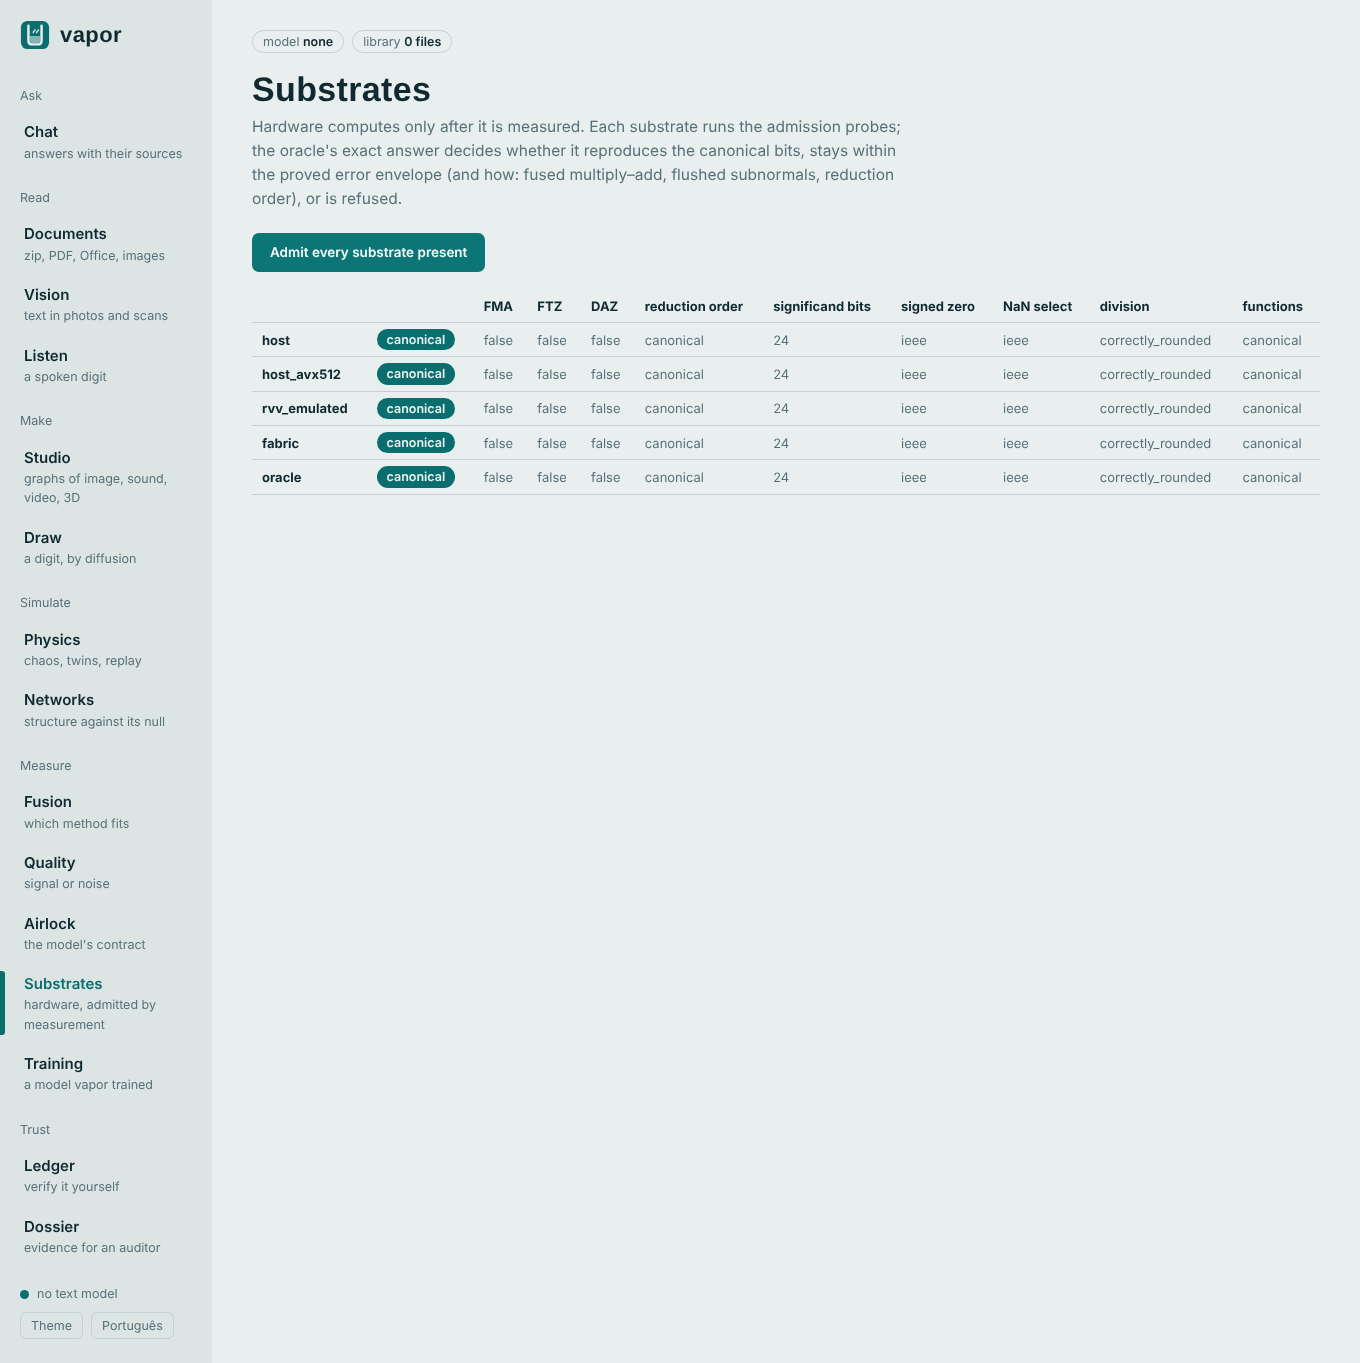
\includegraphics[width=0.78\textwidth]{figuras/console-substratos.png}
\caption{A eclusa de substratos no console: cada substrato com o veredito de admissão e a impressão numérica medida.}
\label{fig:substratos}
\end{figure}

% ----------------------------------------------------------------------------
\section{Modelo numérico}\label{sec:arq-numerico}

O oráculo \code{Vapor.F32} implementa binary32 \emph{exato} na BEAM (\autoref{sec:fp}). Sobre ele, duas políticas (\autoref{tab:politicas}).

\begin{table}[htbp]
\centering
\caption{Políticas numéricas}\label{tab:politicas}
\small
\begin{tabularx}{\textwidth}{@{}lXX@{}}
\toprule
\textbf{política} & \textbf{semântica} & \textbf{garantia}\\
\midrule
\code{:canonical} & multiplicação e soma arredondadas separadamente; redução em árvore fixa de 16 pistas; $\div$ corretamente arredondada; funções transcendentais como microprogramas fixos & \textbf{bits idênticos} em x86, ARM, RVV, interpretador e GPU\\
\code{:fast} & FMA fundida onde o operador permite & dentro do envelope rigoroso em todos os substratos\\
\bottomrule
\end{tabularx}
\end{table}

\paragraph{O envelope.} Para cada saída, \code{Vapor.Verify.Envelope} calcula em racionais diádicos exatos o valor real e uma cota válida para \emph{qualquer} substrato conforme --- arredondamento correto, FMA fundida ou não, qualquer ordem de redução, \textit{underflow} gradual ou FTZ. Para contrações sobre entradas exatas usa a forma de Wilkinson $\gamma_n S + a$ (\autoref{eq:gamma}), decidida pelo \code{within\_envelope/4} extraído do Lean; para o resto, análise de erro corrente. O verificador nunca arredonda; só as cotas são encurtadas, e só para cima.

\paragraph{Versão da semântica.} Os bits de um programa são função dos seus termos \emph{e} da definição das funções canônicas, e os certificados registram a versão. Na versão 1, $a/b = a \cdot \mathrm{rcp}(b)$, a até 1~ulp; desde a versão 2 (rodada 0.6), a divisão é corretamente arredondada (Markstein com resíduo exato de Dekker, sem FMA), de modo que $+$, $-$, $\times$ e $\div$ são IEEE em todo substrato. As transcendentais são idênticas em todo substrato, mas não corretamente arredondadas (até 1--2~ulps, medido).

\begin{graduacao}
\textbf{Reprodutível não é o mesmo que exato.} Os bits canônicos do \vapor{} não são ``o valor real'': são \emph{um} resultado em binary32, sempre o mesmo. O valor real está dentro do envelope. A garantia canônica responde a ``por que deu diferente na outra máquina?'' (não dá); o envelope responde a ``quão longe da verdade pode estar?''.
\end{graduacao}

% ----------------------------------------------------------------------------
\section{Escada de verificação e certificado}\label{sec:arq-escada}

Cada compilação atravessa seis degraus (\autoref{tab:escada}). Os três primeiros são estáticos; os três seguintes executam o código nos substratos disponíveis.

\begin{table}[htbp]
\centering
\caption{A escada de verificação}\label{tab:escada}
\small
\begin{tabularx}{\textwidth}{@{}clX@{}}
\toprule
\textbf{degrau} & \textbf{estabelece} & \textbf{como}\\
\midrule
1 & tipos, formas, realimentação & verificação do programa\\
--- & reescrita exata & só identidades provadas\\
2 & admissão & alocação aceita pelo verificador extraído em toda ISA; ausência de transbordamento int8 no máximo das extensões; limites do SPIR-V\\
3 & identidade adjunta & $\langle Wx, v\rangle = \langle x, W^\top v\rangle$ entre o kernel compilado e a transposta exata (pega erros de \textit{layout})\\
4 & oráculo diferencial & cada substrato de CPU igual, bit a bit, ao oráculo exato\\
5 & paridade + envelope & resumos FNV-1a iguais entre substratos; toda saída dentro do envelope\\
6 & certificado & assinatura Ed25519 com quórum por co-assinatura\\
\bottomrule
\end{tabularx}
\end{table}

O certificado contém o SHA-256 do programa, de cada \textit{blob} de máquina e de cada módulo SPIR-V; o resumo das fontes Lean dos verificadores; as evidências de cada degrau; e o \textbf{trabalho contado} (FLOPs, bytes, instruções por ISA). Ele \emph{não} contém nada que dependa do \textit{host} --- nem tempos, nem a decisão de despacho. Por isso nós independentes que refazem a escada produzem cargas \emph{idênticas byte a byte}, codificadas em CBOR determinístico, e podem co-assinar; a verificação exige um quórum de assinaturas válidas de chaves distintas confiáveis. Um nó de borda confere assinaturas e \textit{hashes} em cerca de 2~ms e executa sem refazer a escada.

\begin{mestrado}
\textbf{Por que tirar a decisão de despacho do certificado.} A versão original da diretriz do projeto pedia que o certificado registrasse em que substrato rodar. Isso tornaria o certificado dependente da máquina que o produziu e impediria a co-assinatura. O escrutínio da diretriz trocou a decisão pelo \emph{trabalho contado}, que é portátil: cada nó toma a sua decisão a partir do trabalho certificado e do seu próprio perfil (\autoref{sec:arq-arbitro}). A lição geral: um certificado deve conter só o que outro verificador independente consegue reproduzir.
\end{mestrado}

% ----------------------------------------------------------------------------
\section{Árbitro: o \textit{roofline} de três tetos}\label{sec:arq-arbitro}

O despachante escolhe o substrato pelo menor tempo previsto
\begin{equation}
  t = \sum_{\text{regiões}} \max\!\left(\frac{F}{\pi}, \frac{Q}{\beta}, \frac{I}{\iota}\right) + \text{sobrecustos},
  \label{eq:roofline}
\end{equation}
em que $F$ e $Q$ são FLOPs e bytes contados do \textit{schedule}, $\pi$ e $\beta$ os tetos de cálculo e de banda do perfil declarado, e $I$ a contagem estática das instruções do corpo de cada laço quente \emph{como emitido}, vezes o número de iterações, sobre a vazão de emissão $\iota$. O terceiro teto é o que torna o modelo honesto: o GEMV de 4~bits é limitado por emissão de instruções (cerca de 1,1 instrução por peso), não por banda, e o modelo de dois tetos de \citeonline{williams2009} erra por cerca de 5$\times$. Com os três, o GEMV $4096 \times 4096$ é previsto em 71,7~ms e observado em 72--75~ms.

% ----------------------------------------------------------------------------
\section{Modelo de garantias}\label{sec:arq-garantias}

Toda afirmação do \vapor{} pertence a uma de quatro classes, e a documentação diz a qual (\autoref{fig:garantias}).

\begin{figure}[htbp]
\centering
\begin{tikzpicture}[font=\footnotesize]
\node[dark, text width=12.2cm, minimum height=9mm] (t) {\textbf{confiado}: a BEAM e o kernel Linux; o \textit{printer} do extrator ($\approx$200 linhas); o modelo padrão da IEEE-754 no \textit{hardware}; o \textit{driver} Vulkan (contido em processo)};
\node[box, below=1.5mm of t, text width=12.2cm, minimum height=9mm] (te) {\textbf{testado}: codificadores (binutils, QEMU, lavapipe); interpretador RVV contra QEMU em VLEN 128/256/512; igualdade bit a bit entre substratos; contenção de falhas; aplicações contra oráculos externos};
\node[acc, below=1.5mm of te, text width=12.2cm, minimum height=9mm] (ex) {\textbf{extraído para Elixir}: \code{check\_alloc}, \code{admissible}, \code{wrap\_s32}, \code{pad\_stride}, \code{bank\_of}, \code{affine\_op}, \code{seg\_affine}, \code{within\_envelope}};
\node[acc, below=1.5mm of ex, text width=12.2cm, minimum height=9mm, fill=vcyan!18] (pr) {\textbf{provado em Lean 4} (sem \code{axiom}/\code{sorry}): $\mathbb{Z}/2^{32}$ e paridade inteira; bancos; monoide afim; verificador de alocação; envelope; Higham; regras de reescrita num modelo IEEE de bits};
\end{tikzpicture}
\caption{As quatro classes de garantia, da base confiável (topo) ao núcleo provado (base).}
\label{fig:garantias}
\end{figure}

O extrator lê os termos \emph{elaborados} do Lean --- os mesmos sobre os quais os teoremas falam --- e falha em qualquer construção fora do fragmento suportado. O Lean calcula mais de 480 vetores de conformidade que o Elixir extraído precisa reproduzir, e o módulo gerado carrega o resumo das fontes Lean, conferido por um teste de auditoria sem precisar do \textit{toolchain}. A extração é de tempo de \textit{build}, não de execução: rodar o Lean em produção reintroduziria a pilha gigante que o projeto quer eliminar.

\begin{doutorado}
\textbf{Quão pequena pode ser a base confiável de um compilador de tensores?} O \vapor{} confia no modelo padrão da IEEE-754 tal como implementado pelo \textit{hardware} e no \textit{printer} do extrator. A primeira suposição poderia ser trocada por testes exaustivos para binary32 (são $2^{64}$ pares para operações binárias --- inviável) ou por uma especificação formal do \textit{hardware}; a segunda, por um extrator verificado. Os codificadores de instruções são \emph{testados} contra o binutils, que é ele mesmo não verificado. Uma linha de pesquisa natural é ligar os codificadores a uma semântica formal de ISA (como as especificações Sail de ARM e RISC-V) e provar que a palavra emitida decodifica para a instrução pretendida. Fica em aberto se isso pode ser feito sem perder a propriedade \code{deps: []} e o custo de compilação baixo.
\end{doutorado}

% ----------------------------------------------------------------------------
\section{Camadas sobre o núcleo}\label{sec:arq-camadas}

As camadas construídas nas treze rodadas usam o núcleo \emph{sem alterá-lo}: tudo que produzem é programa certificado ou dado canônico (\autoref{tab:camadas}). Isso é uma regra de arquitetura verificada por teste --- a rodada 0.6 encontrou e corrigiu uma violação real, em que o motor de geração lia a configuração de uma família de modelo.

\begin{table}[htbp]
\centering
\caption{Camadas sobre o núcleo e a garantia que cada uma herda}\label{tab:camadas}
\small
\begin{tabularx}{\textwidth}{@{}lXX@{}}
\toprule
\textbf{camada} & \textbf{conteúdo} & \textbf{garantia herdada}\\
\midrule
modelos (0.2--0.8) & Llama, Qwen, Mixtral, DeepSeek-V3, Gemma, Phi, Mamba, Whisper, ViT, CLIP, VAE, U-Net, DiT, pela eclusa de modelos & mesmos bits em todo substrato, \textit{thread}, lote e réplica\\
saída restrita (0.3) & gramáticas de bytes sobre o vocabulário (JSON Schema) & só tokens admitidos; nenhum prefixo aceito é beco sem saída\\
agentes e RAG (0.3) & diário encadeado + Merkle + atestado; índices determinísticos & repetir é verificar\\
documentos e OCR (0.4--0.8) & PDF, Office, JPEG, CCITT, JBIG2, tabelas & bit a bit iguais a libjpeg, libtiff, jbig2dec\\
estúdio (0.9) & grafos com cache por conteúdo & raiz de Merkle por execução\\
bancada, engenharia, lógica (0.12) & EDOs, circuitos, estruturas, SAT, LP & certificado calculado fora do \textit{solver}\\
finanças e mesa (0.13) & curvas, opções, Monte Carlo, risco, \textit{backtests}, arbitragem, livro de ofertas & \textbf{compila para o núcleo} (Monte Carlo); CBOR canônico e Merkle (diários)\\
\bottomrule
\end{tabularx}
\end{table}

A rodada 0.13 é a primeira desde a bancada (0.12) a voltar a \emph{compilar para o núcleo}: o passo de uma trajetória de Monte Carlo, inclusive o gerador de números aleatórios, é escrito como termos da álgebra e herda a garantia central. O \autoref{cap:financas} descreve como.

% ============================================================================
\chapter{Inovações}\label{cap:inovacoes}
% ============================================================================

Este capítulo isola as inovações do \vapor{}. Cada uma é apresentada com uma \emph{ficha} que responde às cinco perguntas da \autoref{tab:cinco} --- o quê, para quem, para que, por que, como ---, seguida da evidência que a sustenta e do seu limite. O critério de inclusão é exigente: só entra o que (i) não é prática corrente nos sistemas comparáveis do \autoref{cap:relacionados}, (ii) está implementado e testado no repositório e (iii) tem uma medida que poderia ter falhado.

% ----------------------------------------------------------------------------
\section{Numérica canônica portátil}\label{sec:inov-canonica}

\begin{ficha}{Ficha 1 --- Os mesmos bits em todo substrato}
\textbf{O quê.} Uma semântica de ponto flutuante fixa bit a bit para todos os operadores da álgebra, inclusive divisão e funções transcendentais, realizada igualmente em x86-64 (AVX2, AVX-512), AArch64, RISC-V (VLEN 128 a 512), Vulkan e no oráculo.\\
\textbf{Para quem.} Quem precisa que um resultado numérico seja o mesmo em qualquer máquina: auditoria de modelos de IA, ciência reprodutível, risco financeiro regulado.\\
\textbf{Para que.} Para que ``rodei de novo e deu diferente'' deixe de ser possível e para que a comparação entre máquinas vire um teste de igualdade, não de tolerância.\\
\textbf{Por que.} Porque a irreprodutibilidade vem de escolhas arbitrárias (ordem de redução, FMA, implementação de $\exp$), não de limitações físicas; fixadas as escolhas, a igualdade é de graça.\\
\textbf{Como.} Redução em árvore fixa de 16 acumuladores; multiplicação e soma arredondadas separadamente; divisão corretamente arredondada; transcendentais como microprogramas sobre $+$, $-$, $\times$; paralelismo só entre saídas independentes.
\end{ficha}

A literatura de reprodutibilidade numérica oferece duas respostas: somas reprodutíveis por pré-arredondamento ou acumuladores longos \cite{demmel2015}, que custam um fator constante em cada redução, e modos determinísticos de bibliotecas \cite{pytorchdeterminism}, que garantem igualdade só na mesma máquina e na mesma versão. O \vapor{} toma um terceiro caminho: em vez de tornar a soma insensível à ordem, \emph{fixa a ordem} e tira o paralelismo de outro lugar. Um GEMV tem milhares de linhas independentes; processar $R$ linhas por iteração, cada uma com os seus 16 acumuladores, dá paralelismo de instrução e de \textit{threads} sem tocar em nenhuma soma.

\paragraph{Evidência.} A garantia é testada em todas as formas de paralelismo do sistema (\autoref{tab:invariancias}). Cada linha da tabela é um teste que compara bits, não uma tolerância.

\begin{table}[htbp]
\centering
\caption{Invariâncias testadas bit a bit}\label{tab:invariancias}
\small
\begin{tabularx}{\textwidth}{@{}lX@{}}
\toprule
\textbf{a resposta não depende de} & \textbf{como é testado}\\
\midrule
ISA & AVX2, AVX-512, NEON e RVV (sob QEMU) iguais ao oráculo\\
VLEN do RISC-V & 128, 256 e 512 iguais\\
GPU & Vulkan (lavapipe) igual à CPU no modelo inteiro, com amostragem\\
número de \textit{threads} & 1 = 2 = 3 \textit{threads}\\
lote & tokens de uma sequência iguais sozinha ou num lote contínuo, com qualquer fatiamento do \textit{prefill}\\
lugar do cache & KV paginado igual ao contíguo\\
réplica & qualquer réplica dá a mesma resposta; réplicas entre nós de um \textit{cluster} comparadas bit a bit\\
armazenamento dos pesos & bf16 residente igual a f32 sobre os pesos arredondados\\
especulação & saída da decodificação especulativa (linear e em árvore) igual à do alvo sozinho\\
esparsidade & MoE esparso (e em 4 bits) igual ao denso\\
\bottomrule
\end{tabularx}
\end{table}

\paragraph{Limite.} As transcendentais são iguais em todo lugar mas não corretamente arredondadas (1--2~ulps). A garantia é sobre os substratos medidos; um substrato novo precisa passar pela eclusa (\autoref{sec:inov-eclusas}). O texto normalizado depende da versão do Unicode do OTP, registrada mas não eliminada.

% ----------------------------------------------------------------------------
\section{Desempenho sem reassociar}\label{sec:inov-desempenho}

\begin{ficha}{Ficha 2 --- Velocidade que não troca bits}
\textbf{O quê.} Técnicas de desempenho de fronteira --- MoE esparso, cache latente (MLA), janela deslizante em anel, decodificação especulativa em árvore, paralelismo de tensor, GPU residente --- cada uma reformulada para não mudar um bit.\\
\textbf{Para quem.} Operadores de inferência que hoje escolhem entre velocidade e reprodutibilidade.\\
\textbf{Para que.} Para que otimizar não exija revalidar.\\
\textbf{Por que.} Porque cada uma dessas técnicas é, no fundo, uma escolha de \emph{quais} saídas calcular ou \emph{onde} guardar dados, não de \emph{como} somar.\\
\textbf{Como.} MoE por predicação de linha; paralelismo de tensor por coluna com \textit{all-gather} (nunca por linha com \textit{all-reduce}, que reassociaria); especulação que verifica $k+1$ linhas do alvo num passo; janela como cache circular na tabela de blocos.
\end{ficha}

\paragraph{Evidência.} MoE esparso: 2,6$\times$ no \textit{decode}, bits iguais ao denso. MLA latente: 85$\times$ menos memória de cache. Janela em anel: 7,9$\times$ mais sequências a 32\,k tokens. GPU com sessões residentes: 10--12~ms por token contra 72~ms sem sessão, os bits da CPU. GEMV f32 $2048^2$: 2,24$\times$ com 2 \textit{threads} na mesma máquina de 2 vCPUs, sem mudar um bit.

\paragraph{Limite.} O paralelismo de tensor por linha com \textit{all-reduce}, o mais comum na prática, é recusado; o custo é mais tráfego de rede. O GEMV de 4 bits continua limitado por emissão de instruções.

% ----------------------------------------------------------------------------
\section{Compilar sem confiar no compilador}\label{sec:inov-alocacao}

\begin{ficha}{Ficha 3 --- Alocação sem \textit{spill}, conferida por um verificador provado}
\textbf{O quê.} Um compilador que emite bits de cinco alvos sem assembler, sem C e sem LLVM, em que cada alocação de registradores é aceita só depois de conferida por um verificador provado em Lean e extraído para Elixir.\\
\textbf{Para quem.} Pesquisadores de compiladores verificados; equipes que precisam de uma cadeia de compilação auditável e pequena.\\
\textbf{Para que.} Para que a fase mais propensa a erros sutis (alocação) não precise ser confiada.\\
\textbf{Por que.} Provar uma heurística é caro e frágil; provar o verificador é barato e vale para qualquer heurística.\\
\textbf{Como.} \textit{Linear scan} com blocos alinhados e o fator de grupo $g$ (o LMUL do RVV generalizado a todas as ISAs); sem caminho de \textit{spill} --- falta de registrador muda a forma do código; \code{checkAlloc\_sound} em Lean.
\end{ficha}

O ``sem \textit{spill}'' é uma escolha de primeiros princípios. Um \textit{spill} é uma escrita e uma leitura de memória introduzidas pelo compilador, invisíveis no programa-fonte e difíceis de contar no trabalho certificado. Mudando a forma do código (menos linhas por iteração, grupos menores, fronteiras de região), o compilador mantém o trabalho contado exato e o código sempre dentro dos registradores. A consequência medida está no árbitro: o modelo de três tetos acerta o GEMV de 4 bits porque conta as instruções \emph{como emitidas} (\autoref{sec:arq-arbitro}).

\paragraph{Limite.} O verificador extraído é quadrático; compilar programas grandes desenrolados é lento (cerca de 0,6~s por passo e por ISA no Monte Carlo da rodada 0.13).

% ----------------------------------------------------------------------------
\section{Contenção total do código gerado}\label{sec:inov-contencao}

\begin{ficha}{Ficha 4 --- Nenhum byte emitido executa na máquina virtual}
\textbf{O quê.} Todo código gerado roda em processos do sistema operacional com seccomp, W\^{}X e \textit{watchdog}; funções nativas na VM são proibidas por um teste de auditoria.\\
\textbf{Para quem.} Quem serve modelos ou executa código gerado num serviço de longa duração.\\
\textbf{Para que.} Para que um erro do compilador, do \textit{driver} ou da GPU custe uma requisição, não o serviço.\\
\textbf{Por que.} Porque o compilador não é provado inteiro; a contenção limita o que um erro dele pode fazer.\\
\textbf{Como.} Quadros com comprimento prefixado; tabelas dimensionadas pelo quadro; reinício supervisionado; \textit{failover} que não muda bits.
\end{ficha}

\paragraph{Evidência.} As quatro classes de falha (\code{SIGILL}, \code{SIGSEGV}, \code{SIGALRM}, \code{SIGSYS}) são provocadas nos testes; em todas só o worker morre e a unidade seguinte roda. Um ``interpretador seguro'' em função nativa foi \emph{recusado} no escrutínio da diretriz: compartilharia o espaço de endereçamento da VM.

\paragraph{Limite.} O worker é Linux; um worker para macOS (com \code{MAP\_JIT}, sem seccomp) não foi escrito. Sob \code{qemu-user} o seccomp não está disponível (o isolamento por processo continua).

% ----------------------------------------------------------------------------
\section{Certificados portáteis, co-assináveis e transparentes}\label{sec:inov-certificados}

\begin{ficha}{Ficha 5 --- Um certificado que nós independentes reproduzem byte a byte}
\textbf{O quê.} Um certificado Ed25519 da compilação, sem nenhum dado dependente do \textit{host}, codificado em CBOR determinístico, que vários nós podem refazer e co-assinar, e que pode ser ancorado num log de transparência.\\
\textbf{Para quem.} Cadeias de suprimento de modelos; auditores; reguladores (os dossiês mapeiam cada evidência a dispositivos do AI Act europeu e da ISO/IEC 42001, e dizem onde não há nenhuma).\\
\textbf{Para que.} Para que confiar num binário signifique confiar num quórum, não num fornecedor.\\
\textbf{Por que.} Porque um certificado só tem valor se outro verificador independente consegue reproduzi-lo.\\
\textbf{Como.} Trabalho contado em vez de decisão de despacho; CBOR (RFC 8949 §4.2) em vez de \code{term\_to\_binary}; log Merkle RFC 9162 com \textit{checkpoints} C2SP e testemunhas que recusam retrocesso e bifurcação.
\end{ficha}

\paragraph{Evidência.} Payloads idênticos entre nós; verificação de borda em cerca de 2~ms; num dossiê, nenhuma de 209 alterações de um bit é aceita; o verificador do log roda no próprio navegador.

% ----------------------------------------------------------------------------
\section{Eclusas: admissão por medição}\label{sec:inov-eclusas}

\begin{ficha}{Ficha 6 --- Nada entra sem ser medido na fronteira}
\textbf{O quê.} Três eclusas com a mesma forma: a de \emph{modelos} transforma um \textit{checkpoint} num contrato conferido; a de \emph{substratos} mede um acelerador antes de lhe dar programas; a de \emph{documentos} lê arquivos com a proveniência de cada trecho até a página e o \textit{hash}.\\
\textbf{Para quem.} Quem integra componentes de terceiros --- modelos, aceleradores, documentos.\\
\textbf{Para que.} Para que o núcleo não conheça famílias, fornecedores ou formatos, e para que a recusa venha com o motivo e o reparo.\\
\textbf{Por que.} Porque o custo de integração cresce com o que o núcleo precisa saber; uma eclusa concentra esse conhecimento num lugar só.\\
\textbf{Como.} Contratos (\code{:causal\_lm}, \code{:encoder}, \code{:codec}, \code{:map}); adaptadores por dados (JSON), \textit{blueprint} ou topologia; sondas de resposta conhecida com impressão numérica; leitores próprios de zip, PDF, Office, JPEG, CCITT, JBIG2.
\end{ficha}

\paragraph{Evidência.} Os adaptadores novos são conferidos contra o próprio \code{transformers} --- o que achou um defeito real de \textit{rotary} parcial, admitido e calculado errado em silêncio, num caminho de referência. O decodificador JPEG é igual ao libjpeg bit a bit; CCITT G3/G4, ao libtiff; JBIG2, ao jbig2dec (43 de 43 fluxos).

% ----------------------------------------------------------------------------
\section{Uma busca propõe, um verificador decide --- com controles}\label{sec:inov-proponente}

\begin{ficha}{Ficha 7 --- Toda resposta com o seu juiz, todo juiz com o seu controle}
\textbf{O quê.} Um padrão de arquitetura aplicado a domínios inteiros: o procedimento que produz uma resposta (busca, \textit{solver}, modelo de linguagem, pessoa) é separado do que a confere, e cada verificação é acompanhada de um \emph{controle} --- o valor que uma implementação quebrada produziria --- que mostra que ela poderia ter falhado.\\
\textbf{Para quem.} Quem usa saídas de modelos generativos ou de buscas heurísticas e precisa separar sinal de ruído.\\
\textbf{Para que.} Para que ``a saída parece certa'' seja substituída por ``a saída foi conferida, e a conferência tem poder''.\\
\textbf{Por que.} Porque um verificador sem controle pode estar aceitando tudo; e porque a proposta pode vir de qualquer lugar --- inclusive de um modelo de linguagem --- se o juiz for independente dela.\\
\textbf{Como.} Portões calibrados que \emph{recusam existir} se os controles negativos e positivos se sobrepõem; verificações com valor, controle, limiar e veredito; verificadores pequenos (refutações DRUP, KKT, Kirchhoff, Farkas, motor ingênuo); propostas recebidas pelo MCP.
\end{ficha}

O padrão aparece em três níveis. No \textbf{nível de portão}, um detector de ruído (de texto, imagem ou áudio) é ajustado a controles negativos (ruído, sinal embaralhado, repetição) e positivos (sinal real retido) e se recusa a julgar se a margem entre eles for nula. No \textbf{nível de verificação}, a suíte de qualidade (\code{mix vapor.quality}) tem, em cada linha, um controle; na rodada 0.12 foram 147 verificações, todas aprovadas, e a rodada 0.13 acrescenta 23 (\autoref{cap:avaliacao}). No \textbf{nível de domínio}, cada mesa (lógica, engenharia, ciência, finanças) devolve com a resposta um certificado calculado fora do \textit{solver} --- e aceita a \emph{proposta} de qualquer um, conferindo só ela.

\begin{figure}[htbp]
\centering
\begin{tikzpicture}[node distance=6mm and 9mm, font=\footnotesize]
\node[box] (q) {problema\\(texto)};
\node[box, right=of q, yshift=9mm] (s) {busca / \textit{solver}};
\node[box, right=of q, yshift=-9mm] (m) {pessoa ou modelo\\(MCP)};
\node[box, right=of s, yshift=-9mm] (prop) {proposta +\\certificado};
\node[acc, right=of prop] (v) {verificador\\independente\\(pequeno)};
\node[dark, right=of v] (out) {aceito /\\recusado com motivo};
\node[bad, below=8mm of v] (c) {controle:\\o que um juiz\\quebrado aceitaria};
\draw[arr] (q) -- (s); \draw[arr] (q) -- (m); \draw[arr] (s) -- (prop); \draw[arr] (m) -- (prop);
\draw[carr] (prop) -- (v); \draw[carr] (v) -- (out); \draw[arr, dashed] (c) -- node[lbl, right] {deve ser recusado} (v);
\end{tikzpicture}
\caption{O padrão proponente/verificador com controle. A busca pode ser complexa e não confiável; o verificador é pequeno e independente; o controle mostra que ele tem poder.}
\label{fig:proponente}
\end{figure}

\paragraph{Evidência.} Na lógica, a satisfatibilidade de $S(3) = 13$ é decidida com refutação DRUP e a refutação truncada é rejeitada. Na engenharia, o MEF com elemento QM6 fica a 0,9\% da viga analítica enquanto o Q4 trava a 29\% --- e o certificado de equilíbrio é calculado fora do \textit{solver}. Nas finanças, o juiz ingênuo do livro de ofertas achou um defeito real que o motor de produção e o próprio juiz compartilhavam (\autoref{sec:fin-livro}). A \autoref{fig:logica} mostra a mesa de lógica no console.

\begin{figure}[htbp]
\centering
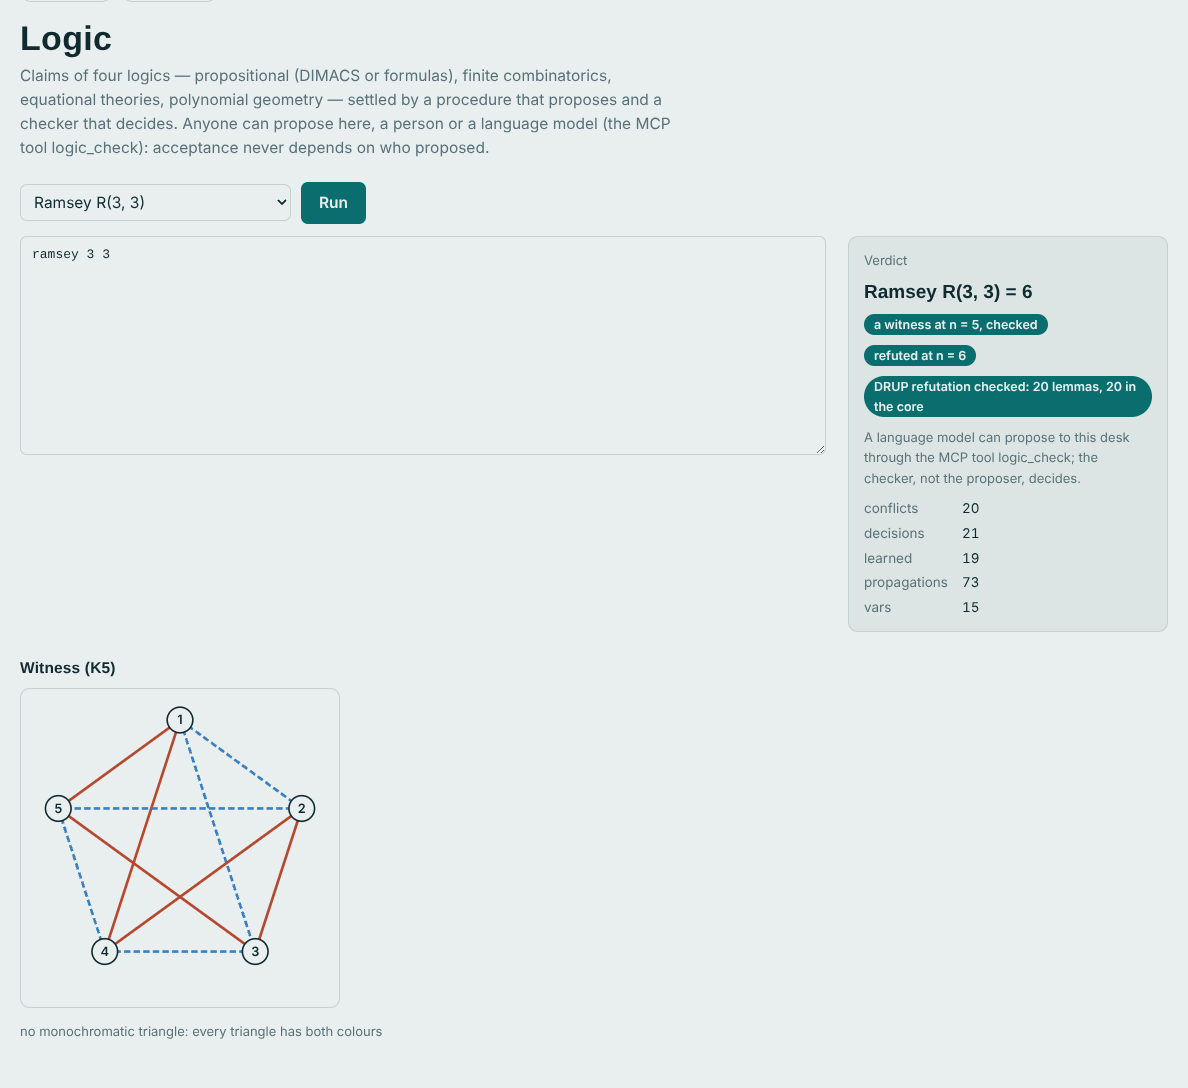
\includegraphics[width=0.78\textwidth]{figuras/console-logica.png}
\caption{A mesa de lógica no console: a afirmação, a decisão e a prova conferível.}
\label{fig:logica}
\end{figure}

\paragraph{Limite.} O padrão exige que exista um verificador mais simples que a busca. Isso vale para problemas em NP e para a otimização convexa (dualidade), mas não para toda pergunta: ``esta estratégia vai dar lucro?'' não tem certificado --- tem, no máximo, portões que dizem quando um \textit{backtest} é indistinguível de ruído (\autoref{sec:fin-backtest}).

% ----------------------------------------------------------------------------
\section{Repetir é verificar}\label{sec:inov-repetir}

\begin{ficha}{Ficha 8 --- Execuções que são objetos de prova}
\textbf{O quê.} Agentes, grafos do estúdio, sessões de bolsa e arquivos salvos cuja execução produz um diário encadeado por \textit{hash}, fechado por uma raiz de Merkle e atestado, de modo que reexecutar é a forma de conferir.\\
\textbf{Para quem.} Quem precisa auditar o que um agente ou um processo automatizado fez.\\
\textbf{Para que.} Para que ``o que aconteceu'' seja recalculável, não narrado.\\
\textbf{Por que.} Porque, com bits canônicos, toda decisão local é re-derivável em qualquer substrato.\\
\textbf{Como.} Diário gravado antes de cada passo; repetição que recalcula sem agir; retomada do disco sem repetir ações; apagamento por titular.
\end{ficha}

A rodada 0.13 estende a ideia ao mercado: a mesma semente de uma sessão de bolsa reproduz \emph{a mesma cabeça de hash} do diário, e outra semente, outra cabeça. Os arquivos salvos das mesas passam a ser \emph{assinados} (Ed25519 sobre \code{"vapor-archive-v1\textbackslash n"} seguido do manifesto), e um manifesto reescrito é recusado.

% ----------------------------------------------------------------------------
\section{Primeiros princípios: as inversões}\label{sec:inov-inversoes}

As inovações acima têm uma raiz comum: cada uma inverte uma suposição que a prática trata como dada. A \autoref{tab:inversoes} as reúne.

\begin{table}[htbp]
\centering
\caption{As suposições usuais e a inversão do \vapor{}}\label{tab:inversoes}
\small
\begin{tabularx}{\textwidth}{@{}XX@{}}
\toprule
\textbf{suposição usual} & \textbf{inversão}\\
\midrule
reprodutibilidade custa desempenho & o paralelismo vem de saídas independentes; a ordem da soma é fixa e de graça\\
o compilador é confiável ou é provado inteiro & o compilador é não confiável; uma fase difícil é conferida por um verificador provado\\
código gerado roda no processo do \textit{runtime} & nenhum byte gerado roda na VM\\
o certificado diz onde rodar & o certificado diz o trabalho; cada nó decide\\
um modelo é aceito porque carrega & um modelo é aceito porque cumpre um contrato conferido contra a referência\\
uma saída boa é uma saída plausível & uma saída boa passou num juiz que tem poder (controle)\\
um \textit{backtest} é um modelo da bolsa & o \textit{backtest} é o código da bolsa (\autoref{sec:fin-sessao})\\
antecipação se evita com disciplina & antecipação se \emph{certifica} ausente, por invariância de prefixo (\autoref{sec:fin-backtest})\\
arbitragem se estima & arbitragem se decide, em racionais, pelo lema de Farkas (\autoref{sec:fin-arbitragem})\\
\bottomrule
\end{tabularx}
\end{table}

\begin{doutorado}
\textbf{Uma teoria dos controles.} A prática de acompanhar cada verificação de um controle que ``deveria ser recusado'' lembra o \textit{mutation testing} e a análise de poder estatístico, mas não é nenhum dos dois: o controle é \emph{escolhido} para representar o erro mais plausível (esquecer o termo de Itô, contar dias corridos em vez de úteis, normalizar pela amostra inteira). Falta uma teoria que diga quais controles bastam para dar a um conjunto de verificações uma garantia de cobertura --- por exemplo, uma noção de ``controle adversarial mínimo'' por classe de erro, com cotas sobre a probabilidade de um defeito passar despercebido. O \vapor{} oferece um corpus de 170 pares (verificação, controle) em domínios variados como ponto de partida empírico.
\end{doutorado}

% ============================================================================
\chapter{Finanças verificáveis: a rodada 0.13}\label{cap:financas}
% ============================================================================

Finanças é o domínio em que ``o número saiu do computador'' vale menos. Um preço que muda quando o cálculo muda de servidor, um \textit{backtest} que olhou o dia seguinte sem querer, a melhor de cinquenta estratégias apresentada como se fosse a única, um livro de ofertas que ninguém de fora consegue auditar: são as dores reais da indústria, e todas são dores de \textbf{verificabilidade}, não de velocidade. Este capítulo descreve como a rodada 0.13 aplica a tese do \autoref{cap:introducao} a esse domínio.

\begin{graduacao}
\textbf{Glossário mínimo.} Uma \emph{mesa} é a equipe (e o sistema) que precifica e negocia instrumentos. \emph{P\&L} é o resultado (\textit{profit and loss}). Um \emph{backtest} simula uma estratégia sobre dados históricos. \emph{Bid} e \emph{ask} são os melhores preços de compra e de venda oferecidos; a diferença é o \emph{spread}. Uma \emph{ordem limitada} só executa ao preço dado ou melhor; uma \emph{ordem a mercado}, ao que houver. HFT (\textit{high-frequency trading}) é a negociação automatizada em escalas de micro a nanossegundos.
\end{graduacao}

% ----------------------------------------------------------------------------
\section{A mesa como arquitetura}\label{sec:fin-mesa}

A \autoref{fig:fin-mesa} mostra o desenho comum a todas as tarefas. O usuário escreve o problema como uma mesa o escreveria --- \code{di1 F26 = 15.02\%}, \code{call S=100 K=100 T=1 r=5\% vol=20\%}, \code{sell 50 @ 101.30 owner=bia} ---; um analisador próprio o lê; um motor o resolve; e a resposta sai com um certificado calculado por um caminho diferente do que a produziu. A mesma entrada chega por quatro portas: a API Elixir (\code{Vapor.Finance.run/2}), a linha de comando (\code{mix vapor.finance}), o console web (\emph{Mercados}) e o servidor MCP, pelo qual um modelo de linguagem pode pedir um cálculo ou submeter uma proposta para conferência.

\begin{figure}[htbp]
\centering
\begin{tikzpicture}[node distance=5mm and 7mm, font=\footnotesize]
\node[box] (api) {API\\Elixir};
\node[box, below=of api] (cli) {\code{mix}\\\code{vapor.finance}};
\node[box, below=of cli] (web) {console\\(Mercados)};
\node[box, below=of web] (mcp) {MCP\\(modelos)};
\node[box, right=10mm of cli, yshift=-5mm] (parse) {texto da mesa\\$\to$ analisador};
\node[box, right=of parse, yshift=10mm] (eng) {motor\\(curva, opção, MC,\\livro, LP\ldots)};
\node[acc, right=of parse, yshift=-10mm] (cert) {certificado\\(outro caminho)};
\node[dark, right=of eng, yshift=-10mm] (ans) {resposta +\\certificado +\\controle};
\node[box, below=8mm of ans] (arc) {arquivo assinado\\(\code{vapor-archive-v1})};
\foreach \n in {api,cli,web,mcp} \draw[arr] (\n.east) -- (parse.west);
\draw[arr] (parse) -- (eng); \draw[arr] (parse) -- (cert); \draw[arr] (eng) -- (ans); \draw[carr] (cert) -- (ans); \draw[arr] (ans) -- (arc);
\draw[arr, dashed] (eng) -- node[lbl, right] {resultado} (cert);
\end{tikzpicture}
\caption{A mesa de finanças: quatro portas, um analisador, um motor e um certificado calculado por outro caminho.}
\label{fig:fin-mesa}
\end{figure}

A \autoref{tab:fin-tarefas} resume as tarefas e o objeto que permite julgar cada resposta. As seções seguintes descrevem cada uma.

\begin{table}[htbp]
\centering
\caption{Tarefas da mesa e o certificado de cada uma}\label{tab:fin-tarefas}
\small
\begin{tabularx}{\textwidth}{@{}lX@{}}
\toprule
\textbf{tarefa} & \textbf{certificado}\\
\midrule
calendário e dinheiro & feriados por regra, iguais ao QuantLib por 89 anos; rateio que soma exatamente\\
curva & todo instrumento reprecificado; \textit{forwards} negativos apontados\\
opções & paridade; gregas contra diferenças finitas; limites de não arbitragem \emph{antes} de resolver; $g(k)$ de Durrleman\\
Monte Carlo & bits = oráculo exato = outra contagem de \textit{threads}; intervalo de 99\% contra a forma fechada\\
risco & Kupiec, Christoffersen, zona de Basileia; tamanho e poder medidos\\
carteira & condições KKT; contribuições de risco iguais aos orçamentos\\
\textit{backtest} & quatro portões: invariância de prefixo, Sharpe deflacionado, PBO, \textit{Reality Check}\\
arbitragem & \emph{ou} o portfólio de arbitragem \emph{ou} os preços de estado, em racionais exatos\\
livro de ofertas & diário SHA-256 + raiz de Merkle; motor ingênuo independente; feed ITCH; FIX\\
sessão de bolsa & os três certificados do livro + a mesma cabeça de \textit{hash} ao repetir\\
microestrutura & teste de reescala do tempo; o artigo reproduzido; forma fechada = ótimo numérico\\
\bottomrule
\end{tabularx}
\end{table}

% ----------------------------------------------------------------------------
\section{Dinheiro exato e calendários por regra}\label{sec:fin-dinheiro}

\paragraph{Dinheiro.} Um valor monetário é um inteiro e uma escala decimal: $\{c = 12345, e = 2\}$ representa 123,45. Soma, subtração e produto são exatos; todo arredondamento é um ato explícito com modo nomeado (\textit{half-even}, \textit{half-up}, \textit{down}, \textit{floor}\ldots), implementado por uma única primitiva testada nos empates dos dois lados do zero. O rateio usa o método do \emph{maior resto} (Hamilton): R\$~100,00 em três partes dá 33,34 + 33,33 + 33,33, e a soma é o total \emph{por construção}; o certificado diz também que cada parte está a menos de uma unidade da sua fração exata. O controle: o mesmo rateio por piso em binary64 perde um centavo (99,99).

O fator da convenção brasileira, $(1 + r)^{\mathrm{DU}/252}$, é calculado com uma raiz inteira em aritmética de inteiros grandes e \emph{truncado} na oitava casa, como faz a ANBIMA. Para $r = 13{,}65\%$ e um dia útil, $(1{,}1365)^{1/252} = 1{,}00050788\ldots$; o módulo \code{decimal} do Python com 60 dígitos concorda --- a decisão na oitava casa não é um acidente de ponto flutuante.

\paragraph{Calendários.} Cada feriado é uma \emph{regra}: data fixa, $n$-ésimo dia da semana, ou festa móvel pelo cômputo gregoriano. A Páscoa sai do algoritmo anônimo de 1876 (Meeus/Jones/Butcher); o Carnaval é a Páscoa menos 48 e 47 dias; a Sexta-feira Santa, menos 2; Corpus Christi, mais 60. Os fechamentos que nenhuma regra produz (11 de setembro de 2001, o furacão Sandy, dias de luto presidencial) são \emph{dados}, cada um com o motivo. A \autoref{tab:calendarios} mostra a conferência contra o QuantLib \cite{quantlib}.

\begin{table}[htbp]
\centering
\caption{Calendários conferidos dia a dia contra o QuantLib 1.43}\label{tab:calendarios}
\small
\begin{tabularx}{\textwidth}{@{}lXr@{}}
\toprule
\textbf{calendário} & \textbf{regras} & \textbf{feriados em dia útil idênticos}\\
\midrule
ANBIMA (= B3) & nacionais + móveis; 20 de novembro desde 2024 (Lei 14.759/2023) & 903 (1990--2078)\\
NYSE & datas observadas; MLK desde 1998; Juneteenth desde 2022; fechamentos especiais & 848\\
TARGET & Sexta Santa, Segunda de Páscoa, 1º de maio e 26 de dezembro desde 2000 & 401\\
\bottomrule
\end{tabularx}
\end{table}

Na primeira comparação, a NYSE divergiu num único dia --- 27/04/1994, o luto pelo presidente Nixon --- e o TARGET em datas anteriores a 2000, quando o sistema não existia. As duas diferenças viraram dado e regra, e o teste passou a exigir igualdade dia a dia. As seis bases de contagem (DU/252, ACT/360, ACT/365F, 30/360, 30E/360, ACT/ACT ISDA) concordam com o QuantLib a $10^{-14}$ nos casos de borda.

\begin{graduacao}
\textbf{Por que dinheiro não é \texttt{double}.} 0,1 não tem representação binária finita. Somar dez vezes 0,10 em binary64 não dá exatamente 1,00, e um rateio feito com pisos em binary64 pode perder um centavo. O erro é minúsculo por operação, mas é um erro \emph{contábil}: o total não fecha. Inteiros com escala decimal fecham por construção.
\end{graduacao}

% ----------------------------------------------------------------------------
\section{Curvas de juros}\label{sec:fin-curvas}

A curva é escrita como uma mesa a escreve (\autoref{fig:fin-curva}). O \textit{bootstrap} põe um nó no último fluxo de cada instrumento e acha, pelo método de Brent, o fator de desconto que o reprecifica, com os nós anteriores fixos. A interpolação é \textit{flat-forward} (log-linear no desconto, a convenção da curva DI) ou linear na taxa zero. Os fluxos seguem as convenções publicadas: o DI1 tem PU $100\,000/(1+r)^{\mathrm{DU}/252}$; a LTN paga 1\,000 no dia útil seguinte ao vencimento; a NTN-F paga cupom semestral $1\,000 \cdot (\sqrt{1{,}1} - 1)$.

\paragraph{O certificado} reprecifica cada instrumento a partir da curva pronta e dá o pior erro relativo ($4{,}5 \cdot 10^{-16}$ na curva DI do exemplo); lista os \textit{forwards} entre nós e \emph{aponta os negativos}. O exemplo ``cotação inconsistente'' (janeiro a 15\%, julho a 9\%) é reprecificado, mas sai com o \textit{forward} negativo nomeado: reprecificar não basta para uma curva ser plausível, e o certificado diz as duas coisas. O controle: o mesmo DI1 contado em dias corridos erra o PU em $2{,}5 \cdot 10^{-3}$. Depósitos simples conferem com o \code{PiecewiseLogLinearDiscount} do QuantLib a $10^{-13}$.

\begin{figure}[htbp]
\centering
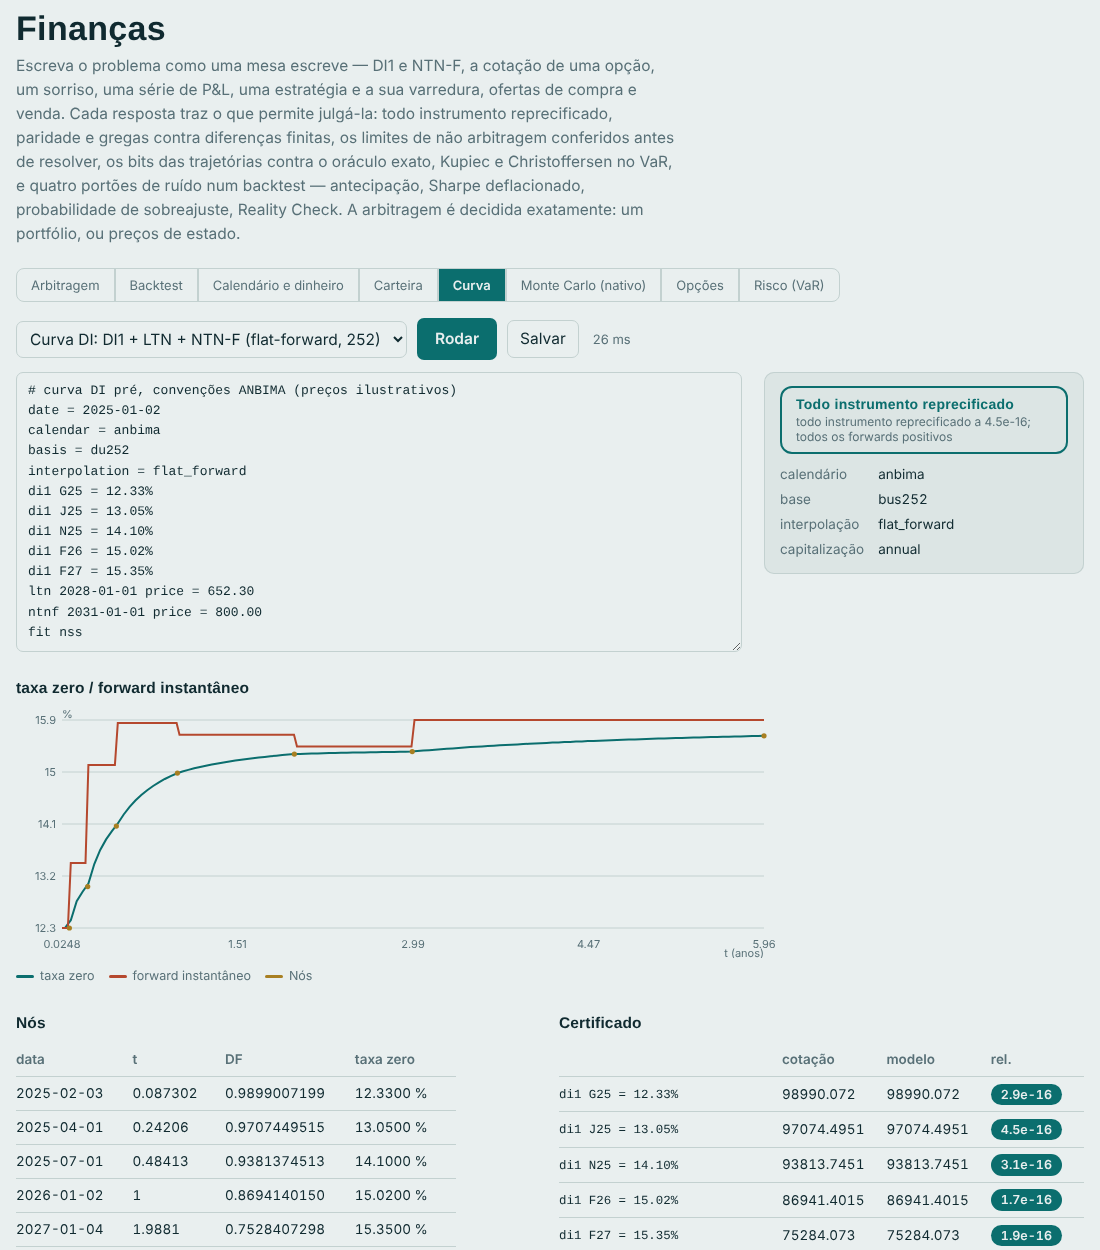
\includegraphics[width=0.82\textwidth]{figuras/console-financas-curva.png}
\caption{Curva DI (DI1 + LTN + NTN-F, \textit{flat-forward}, DU/252) no console: taxa zero, \textit{forward} instantâneo, nós e o certificado de reprecificação.}
\label{fig:fin-curva}
\end{figure}

% ----------------------------------------------------------------------------
\section{Opções}\label{sec:fin-opcoes}

O módulo de opções cobre Black--Scholes--Merton com dividendos \cite{black1973,merton1973}, Black-76, Bachelier (taxas negativas), árvores de Cox--Ross--Rubinstein e Leisen--Reimer \cite{leisen1996}, Heston \cite{heston1993} pela integral de Lewis com a função característica ``\textit{little trap}'' \cite{albrecher2007}, e o sorriso SVI \cite{gatheral2014}. Duas decisões de projeto merecem destaque.

\paragraph{Limites antes de resolver.} A volatilidade implícita é a raiz de $\mathrm{BSM}(\sigma) = p$. Para uma \textit{call}, $\mathrm{BSM}$ é estritamente crescente em $\sigma$ e
\begin{equation}
  \max\!\left(S e^{-qT} - K e^{-rT}, 0\right) < \mathrm{BSM}(\sigma) < S e^{-qT}, \qquad \sigma \in (0, \infty).
  \label{eq:limites}
\end{equation}
Um preço fora desse intervalo não tem volatilidade implícita --- e não é ``mal condicionado'': é uma arbitragem. O \vapor{} confere os limites \emph{antes} de chamar o \textit{solver} e recusa com o limite violado; dentro deles, devolve o erro de reprecificação, a vega e quanto um \textit{tick} de preço move $\sigma$ (o condicionamento, em unidades de mercado).

\paragraph{Arbitragem de borboleta no sorriso.} Uma fatia do SVI dá a variância total $w(k)$ em função do \textit{log-strike} $k$. \citeonline{gatheral2014} mostram que a densidade neutra ao risco implícita é não negativa se e só se
\begin{equation}
  g(k) = \left(1 - \frac{k\, w'(k)}{2\, w(k)}\right)^{\!2} - \frac{w'(k)^2}{4}\left(\frac{1}{w(k)} + \frac{1}{4}\right) + \frac{w''(k)}{2} \;\geq\; 0.
  \label{eq:durrleman}
\end{equation}
O \vapor{} avalia $g$ numa grade fina e devolve o intervalo em que ela é negativa. A fatia que \citeonline{gatheral2014} atribuem a Vogt --- o exemplo clássico de arbitragem de borboleta --- é detectada ($g$ mínimo $-0{,}033$ em $k \in [0{,}645;\, 1{,}255]$); um sorriso calmo ajustado sai com $g \geq 0$ (\autoref{fig:fin-sorriso}).

\begin{figure}[htbp]
\centering
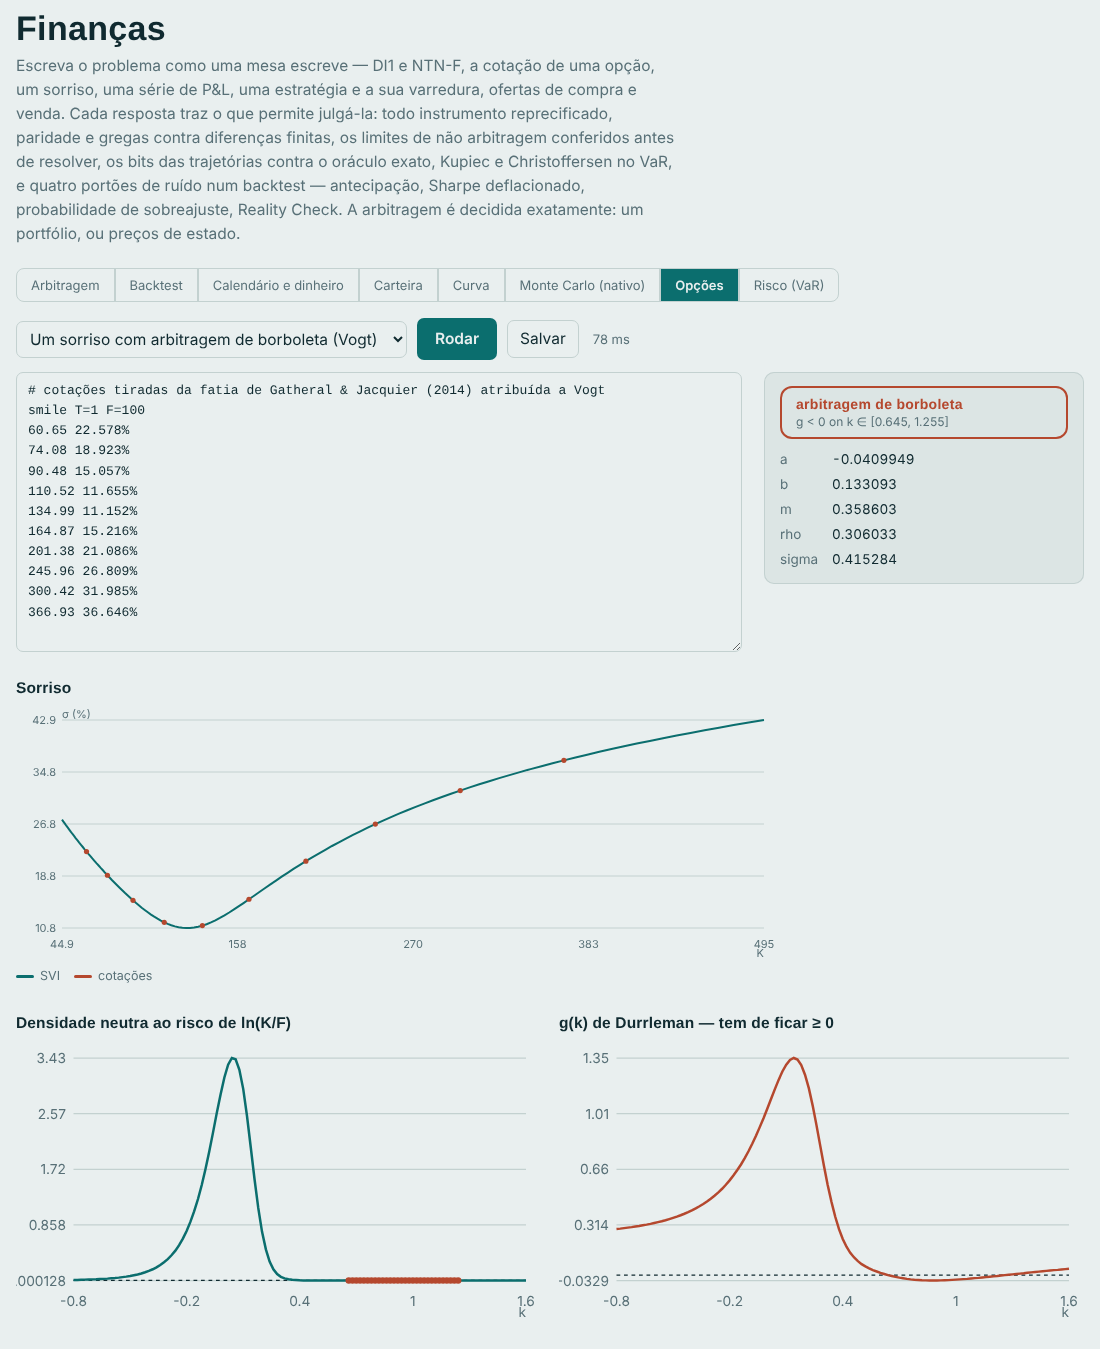
\includegraphics[width=0.82\textwidth]{figuras/console-financas-sorriso.png}
\caption{O sorriso de Vogt: o ajuste SVI, a densidade neutra ao risco (negativa onde há arbitragem) e $g(k)$ de Durrleman abaixo de zero.}
\label{fig:fin-sorriso}
\end{figure}

\paragraph{Contra o QuantLib.} BSM, $\Delta$ e $\Gamma$ a $10^{-12}$, vega a $10^{-10}$; americana de Leisen--Reimer com 801 passos a $10^{-10}$ (4,486076, a \textit{put} da tabela~1 de \citeonline{longstaff2001}); Heston a $10^{-9}$ (o integrador adaptativo de Gauss--Kronrod do QuantLib e a Gauss--Legendre composta daqui concordam até a nona casa). O CRR daqui é o de livro-texto e o do QuantLib usa a aproximação aditiva em log; diferem em $1{,}6 \cdot 10^{-5}$, e a documentação diz qual é qual. O LSM de \citeonline{longstaff2001} sobre a mesma \textit{put} dá $4{,}4788 \pm 0{,}0143$ (o artigo: 4,472).

% ----------------------------------------------------------------------------
\section{Monte Carlo compilado para o núcleo}\label{sec:fin-mc}

A dor: um número de risco que muda quando o cálculo muda de máquina, de contagem de \textit{threads} ou para uma GPU --- reduções paralelas em outra ordem, uma FMA aqui e não ali, outro $\exp$. A resposta do \vapor{}: escrever o passo da trajetória como termos da álgebra e herdar a garantia central.

\paragraph{O passo.} Para o log-preço $L$, com $\mu\Delta = (r - q - \sigma^2/2)\Delta$ e $\sigma\sqrt{\Delta}$ pré-calculados, o programa recorrente atualiza, por trajetória e por passo,
\begin{equation}
  L \leftarrow L + \mu\Delta + \sigma\sqrt{\Delta}\,\Phi^{-1}(u), \quad A \leftarrow A + e^{L}, \quad G \leftarrow G + L, \quad v \leftarrow v \cdot [L > \ln(B/S_0)],
  \label{eq:passo-mc}
\end{equation}
em que $A$ e $G$ acumulam as médias aritmética e geométrica (opções asiáticas) e $v$ marca as trajetórias vivas acima de uma barreira $B$. $\Phi^{-1}$ é o algoritmo AS241 de \citeonline{wichura1988} (PPND7, 7 dígitos --- o que binary32 comporta), com $\log$ e $\mathrm{rsqrt}$ canônicos.

\paragraph{O gerador dentro da álgebra.} Para que a trajetória inteira rode no worker, o gerador também precisa ser termo da álgebra --- e exato em binary32. O \vapor{} usa o gerador de \citeonline{wichmann1982}: três geradores de Lehmer
\begin{equation}
  s_1 \leftarrow 171\, s_1 \bmod 30269, \quad s_2 \leftarrow 172\, s_2 \bmod 30307, \quad s_3 \leftarrow 170\, s_3 \bmod 30323,
\end{equation}
combinados como $u = (s_1/30269 + s_2/30307 + s_3/30323) \bmod 1$.

\begin{proposicao}\label{prop:wh}
Cada atualização de estado do gerador de Wichmann--Hill é calculada exatamente em binary32 pelo programa
\[
p = a \cdot s,\qquad q = \lfloor p \oslash m \rfloor,\qquad s' = p - m \cdot q,
\]
em que $\oslash$ é a divisão corretamente arredondada e $\lfloor y \rfloor$ é calculado por $r = (y \oplus 2^{23}) \ominus 2^{23}$, seguido de $r \ominus 1$ quando $r > y$.
\end{proposicao}

\begin{proof}[Esboço]
Os produtos $a \cdot s$ são inteiros menores que $171 \cdot 30268 = 5\,175\,828 < 2^{23}$ (e analogamente para os outros dois), logo representáveis exatamente com 24 bits de significando: $p$ é exato. Para $0 \leq y < 2^{23}$, somar $2^{23}$ leva $y$ ao binade $[2^{23}, 2^{24})$, em que o ulp é 1; o arredondamento ao mais próximo produz o inteiro mais próximo de $y$, e subtrair $2^{23}$ é exato (Sterbenz). Se o arredondamento subiu, $r > y$ e a correção desce um. O quociente $p/m$ nunca é inteiro (pois $m$ é primo e $0 < s < m$) e, para estes três módulos, nunca arredonda para o inteiro seguinte --- o que se confere exaustivamente, para os cerca de 91 mil estados possíveis ---, de modo que $\lfloor p \oslash m \rfloor = \lfloor p/m \rfloor$; dois seletores no programa corrigem $s'$ para $[0, m)$ por segurança. Finalmente, $m \cdot q \leq p < 2^{23}$ é exato e a subtração de inteiros abaixo de $2^{23}$ também.
\end{proof}

O resultado é que a BEAM só semeia: sementes, geração, transformação normal, passo e acumulação rodam no worker, com os mesmos bits em todo substrato.

\paragraph{Certificados, na mesma resposta.} (i) A primeira chamada, compilada para 64 pistas e rodada pelo \emph{oráculo exato}, é igual bit a bit às 64 primeiras pistas do worker. (ii) A simulação inteira, repetida num worker com 2 \textit{threads}, dá os mesmos bits. (iii) As mesmas uniformes em binary64 na BEAM, com $\Phi^{-1}$ de precisão total, diferem no máximo $2 \cdot 10^{-5}$ no \textit{payoff}. (iv) O intervalo de 99\% contém a forma fechada --- BSM para a europeia, \citeonline{kemna1990} para a asiática geométrica discreta. (v) A asiática aritmética usa a geométrica como variável de controle, com variância dividida por cerca de 1\,300. \textbf{O controle:} esquecer o $-\sigma^2/2$ de Itô em $\mu\Delta$ dá $z = 8{,}7$ --- o estimador viciado é pego, não promediado.

\begin{figure}[htbp]
\centering
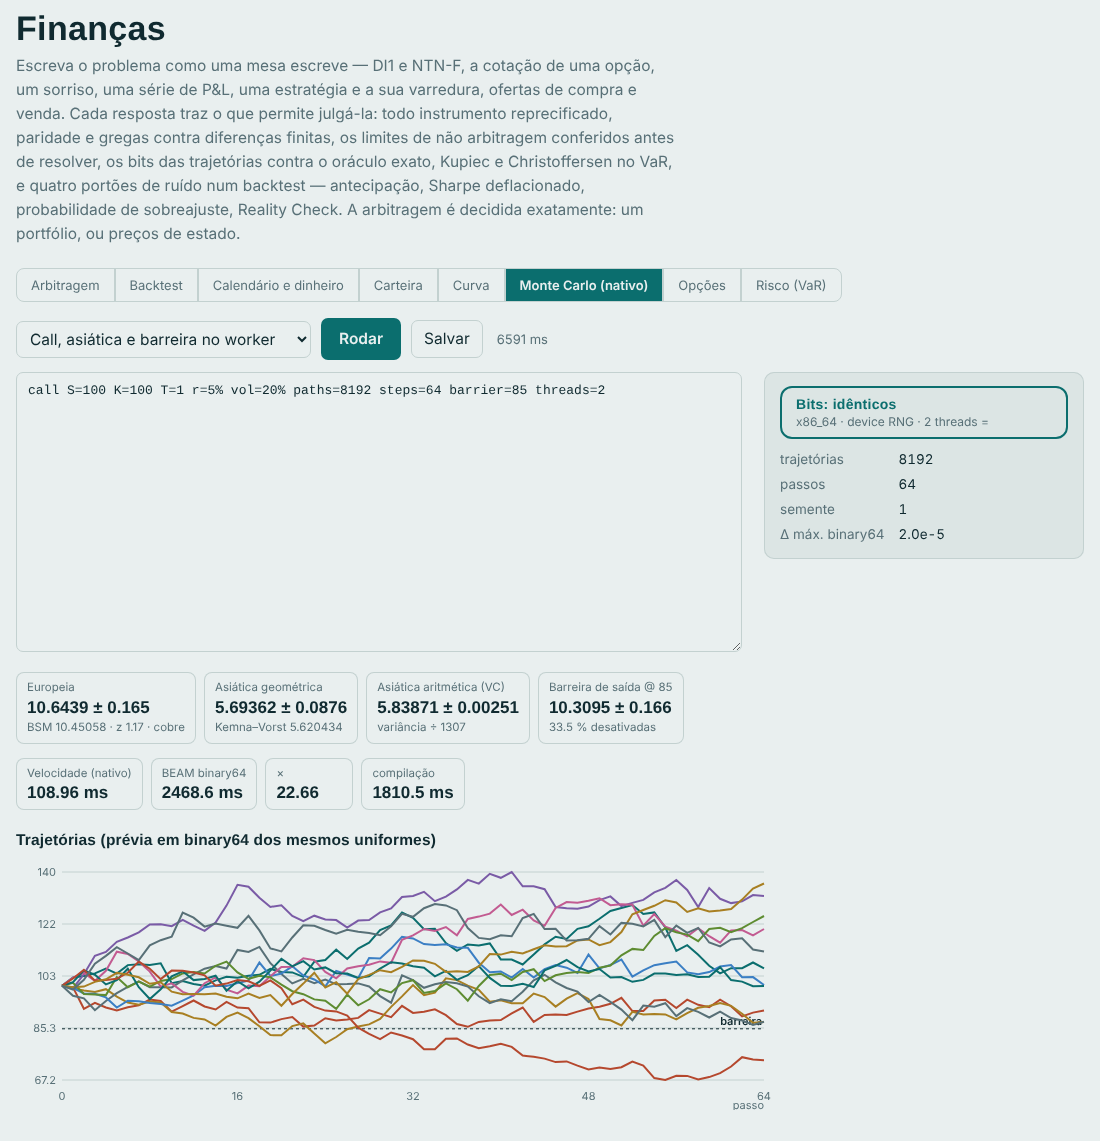
\includegraphics[width=0.82\textwidth]{figuras/console-financas-montecarlo.png}
\caption{Monte Carlo no worker nativo: europeia, asiáticas e barreira, com o selo de bits idênticos (oráculo e 2 \textit{threads}) e a comparação com a BEAM em binary64.}
\label{fig:fin-mc}
\end{figure}

\paragraph{Desempenho.} Numa máquina de 2 vCPUs com AVX-512, um núcleo do worker: 8\,192 trajetórias $\times$ 64 passos em 125~ms, contra 750~ms estimados para a BEAM em binary64 (6$\times$); 16\,384 $\times$ 32 em 86~ms contra 1\,950~ms (23$\times$). A compilação custa cerca de 0,6~s por passo desenrolado e por ISA, por causa do verificador de alocação quadrático (\autoref{sec:inov-alocacao}); por isso o programa tem um passo por chamada e compila só para a ISA da máquina.

\paragraph{Limite.} Wichmann--Hill é um gerador antigo: período de cerca de $7 \cdot 10^{12}$ e falha em baterias modernas como a BigCrush \cite{lecuyer2007}. Serve à precificação, não à criptografia nem a estudos de cauda extrema; a opção \code{rng: :host} usa \textit{splitmix64} na BEAM e compara.

\begin{doutorado}
\textbf{Geradores modernos exatos em binary32.} A restrição ``produtos abaixo de $2^{23}$'' exclui os geradores de qualidade atual (PCG, Philox, xoshiro), que dependem de aritmética inteira de 32 ou 64 bits. A álgebra do \vapor{} tem um gerador \code{gemm\_i8} em $\mathbb{Z}/2^{32}\mathbb{Z}$, com paridade inteira provada em Lean. Fica em aberto se um gerador contrabaseado como o Philox \cite{salmon2011} pode ser expresso com esses operadores inteiros, mantendo a exatidão e a igualdade em GPU, e qual o custo comparado ao Wichmann--Hill em ponto flutuante.
\end{doutorado}

% ----------------------------------------------------------------------------
\section{Risco de mercado e carteiras}\label{sec:fin-risco}

O VaR é calculado pelos métodos histórico, normal, Cornish--Fisher e EWMA ($\lambda = 0{,}94$), em janela móvel, e testado. Se $x$ exceções ocorrem em $n$ dias para um VaR de cobertura $1 - p$, a estatística de \citeonline{kupiec1995} é
\begin{equation}
  \mathrm{LR}_{\mathrm{pof}} = -2 \ln\!\left[(1-p)^{n-x} p^{x}\right] + 2 \ln\!\left[\left(1 - \tfrac{x}{n}\right)^{n-x}\left(\tfrac{x}{n}\right)^{x}\right] \;\sim\; \chi^2_1,
\end{equation}
e a de \citeonline{christoffersen1998} testa, por uma cadeia de Markov de dois estados, se as exceções se agrupam. A zona de Basileia (verde 0--4, amarela 5--9, vermelha $\geq$ 10 exceções em 250 dias a 99\%) acompanha \cite{basel1996}.

\paragraph{Tamanho e poder.} Um teste que nunca rejeita é tão suspeito quanto um que sempre rejeita. O \vapor{} mede o \emph{tamanho} do Kupiec sorteando exceções a exatamente 1\% em 400 séries (rejeita em 1,5--10\% delas) e o seu \emph{poder} numa série de retornos $t$ de Student com $\nu = 3$: o VaR normal é rejeitado ($p = 0{,}038$) e o histórico não ($p = 0{,}43$) (\autoref{fig:fin-var}).

\begin{figure}[htbp]
\centering
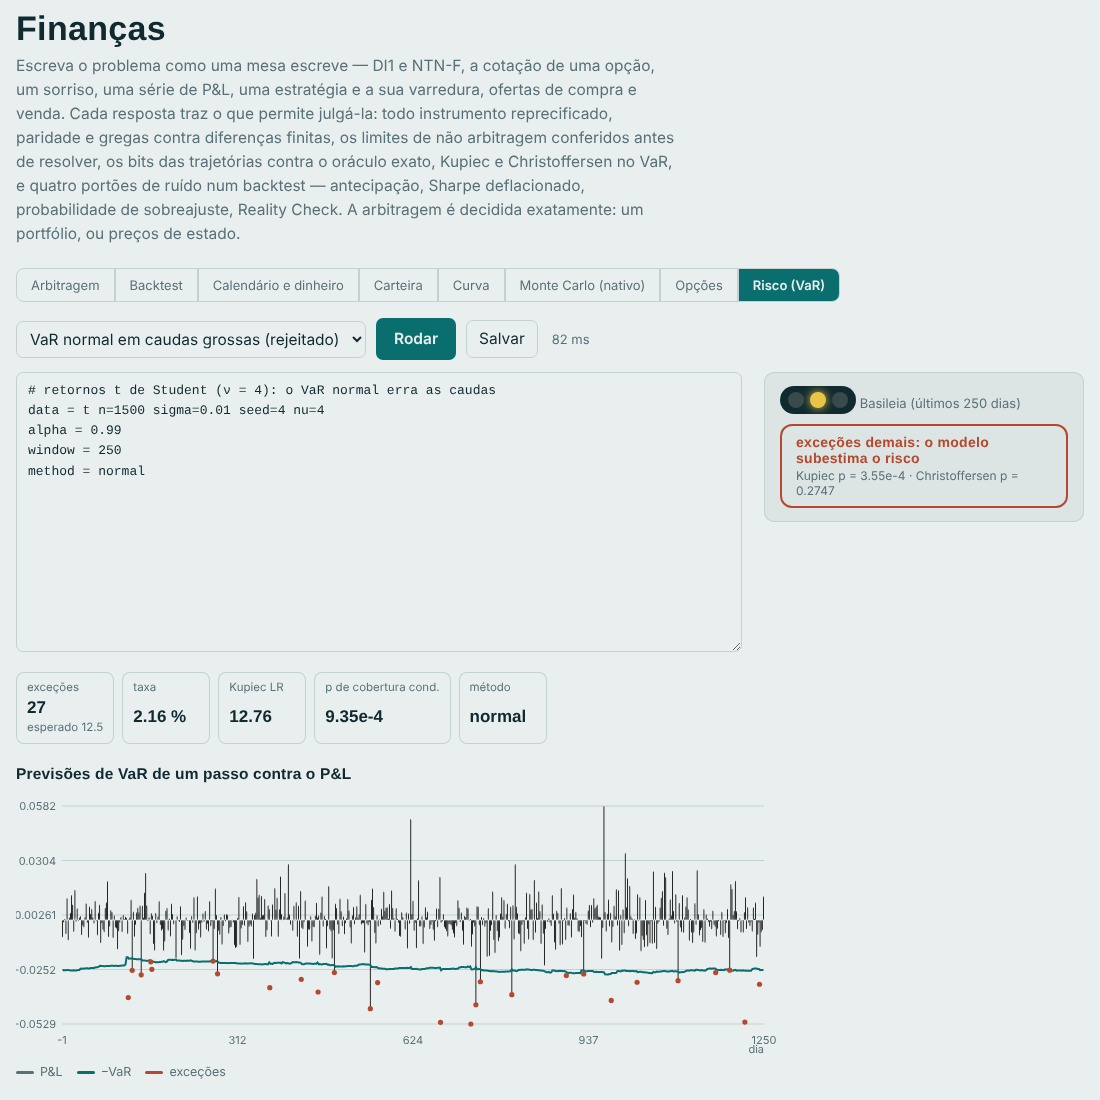
\includegraphics[width=0.82\textwidth]{figuras/console-financas-var.png}
\caption{VaR normal em caudas grossas: as previsões de um passo, as exceções, os testes de Kupiec e Christoffersen e a zona de Basileia.}
\label{fig:fin-var}
\end{figure}

\paragraph{Carteiras.} Covariância encolhida de \citeonline{ledoit2004}; \emph{variância mínima só compra} por conjunto ativo, com as condições KKT como certificado (estacionaridade abaixo de $10^{-12}$, multiplicadores com o sinal certo); \emph{paridade de risco} por Newton na formulação convexa de \citeonline{spinu2013}, com contribuições iguais aos orçamentos a $10^{-12}$; e HRP de \citeonline{lopezdeprado2016}.

% ----------------------------------------------------------------------------
\section{\textit{Backtests} com portões de ruído}\label{sec:fin-backtest}

Um \textit{backtest} é uma máquina de produzir índices de Sharpe; tentando variantes bastantes, uma parecerá boa sobre puro ruído. As duas falhas silenciosas da indústria são a \textbf{antecipação} (o sinal usou informação que não teria) e a \textbf{seleção} (a melhor de muitas tentativas apresentada como a única) \cite{bailey2014pbo,harvey2016}. O \vapor{} trata as duas com quatro portões.

A estratégia é escrita numa linguagem pequena:
\begin{lstlisting}
data = ar1 n=5040 phi=0.15 sigma=0.01 seed=3
sweep k = 1..3
signal = sign(sma(ret(close), k))
cost = 1bp
\end{lstlisting}
Os operadores são causais (\code{lag}, \code{diff}, \code{ret}, \code{sma}, \code{ema}, \code{std}, \code{zscore}, \code{rsi}, \code{sign}, \code{if}\ldots), mas a linguagem aceita, porque as pessoas os escrevem, três que espiam: \code{lead}, \code{center} e \code{normalize} pela amostra inteira. A posição em $(t, t+1]$ é o sinal em $t$; o custo incide sobre $|\Delta\text{posição}|$.

\subsection{Portão 1: invariância de prefixo}

\begin{definicao}[Causalidade observável]
Seja $f$ o \textit{pipeline} que leva uma série de preços $x_{0..n}$ a uma série de sinais $f(x)_{0..n}$. Diz-se que $f$ é \emph{causal} se, para todo $c \leq n$ e todo $t \leq c$, $f(x_{0..c})_t = f(x_{0..n})_t$.
\end{definicao}

\begin{proposicao}\label{prop:prefixo}
Se $f$ é causal, então para qualquer conjunto de cortes $C$ o teste ``$f(x_{0..c})_{0..c} = f(x_{0..n})_{0..c}$ bit a bit para todo $c \in C$'' aceita. Reciprocamente, se o teste rejeita em $c$, existe $t \leq c$ em que o sinal calculado com a história inteira difere do que seria calculado com os dados disponíveis em $c$: $f$ usa informação posterior a $c$.
\end{proposicao}

A proposição é imediata, e é o seu caráter de \emph{caixa-preta} que a torna útil: o teste não precisa conhecer nem confiar nos operadores --- trata o \textit{pipeline} inteiro, inclusive o analisador e o avaliador, como função. Um primeiro rascunho da ideia conferia só os operadores, e teria deixado passar o \code{center}, que é causal em cada passo e não causal no todo (a média é da amostra inteira). Por isso o teste é sobre o resultado, não sobre a gramática. A igualdade é bit a bit porque o avaliador é determinístico; com aritmética não reprodutível, seria preciso uma tolerância, e uma antecipação pequena poderia se esconder nela. O \vapor{} usa oito cortes e devolve o \emph{dia} em que o sinal muda.

\begin{mestrado}
\textbf{Completude.} O teste é correto (nunca acusa um \textit{pipeline} causal) mas não completo: uma antecipação que só se manifeste entre dois cortes, ou que mude o sinal sem mudar o seu valor arredondado, passa. Com $C = \{0, \ldots, n\}$ o teste é completo para a definição acima, ao custo de $n$ avaliações. Os oito cortes são um compromisso; como o custo de cada avaliação é linear, cortes adicionais podem ser pedidos.
\end{mestrado}

\subsection{Portões 2--4: seleção}

O \textbf{Sharpe deflacionado} \cite{bailey2014dsr} é a probabilidade de o Sharpe verdadeiro exceder o máximo esperado de $N$ tentativas sem habilidade:
\begin{equation}
  \mathrm{DSR} = \Phi\!\left(\frac{(\widehat{SR} - SR_0)\sqrt{T-1}}{\sqrt{1 - \hat\gamma_3 \widehat{SR} + \frac{\hat\gamma_4 - 1}{4}\widehat{SR}^2}}\right),
\end{equation}
\begin{equation}
  SR_0 = \sqrt{V}\left[(1-\gamma)\,\Phi^{-1}\!\left(1 - \tfrac{1}{N}\right) + \gamma\, \Phi^{-1}\!\left(1 - \tfrac{1}{N e}\right)\right],
\end{equation}
em que $V$ é a variância dos Sharpes entre tentativas, $\gamma \approx 0{,}5772$ é a constante de Euler--Mascheroni e $\hat\gamma_3, \hat\gamma_4$ são assimetria e curtose. $N$ inclui as tentativas declaradas antes do arquivo (\code{trials =}). A \textbf{probabilidade de sobreajuste} (PBO) por validação cruzada combinatória \cite{bailey2014pbo} divide a série em 16 blocos e, nas $\binom{16}{8} = 12\,870$ metades, mede com que frequência o campeão dentro da amostra cai abaixo da mediana fora dela. O \textbf{\textit{Reality Check}} de \citeonline{white2000} testa se a melhor estratégia supera a nula com o \textit{bootstrap} estacionário de \citeonline{politis1994}.

\paragraph{Medido.} O melhor de 30 cruzamentos de médias sobre um passeio aleatório tem Sharpe positivo e DSR 0,10 --- reprovado (\autoref{fig:fin-backtest}). O sinal plantado (momento sobre AR(1) com $\phi = 0{,}15$) passa os quatro portões (DSR 1,0; PBO $< 0{,}5$; \textit{Reality Check} $p < 0{,}05$). \code{sign(lead(close) - close)} tem Sharpe anual 20 e é pego no dia 89.

\begin{figure}[htbp]
\centering
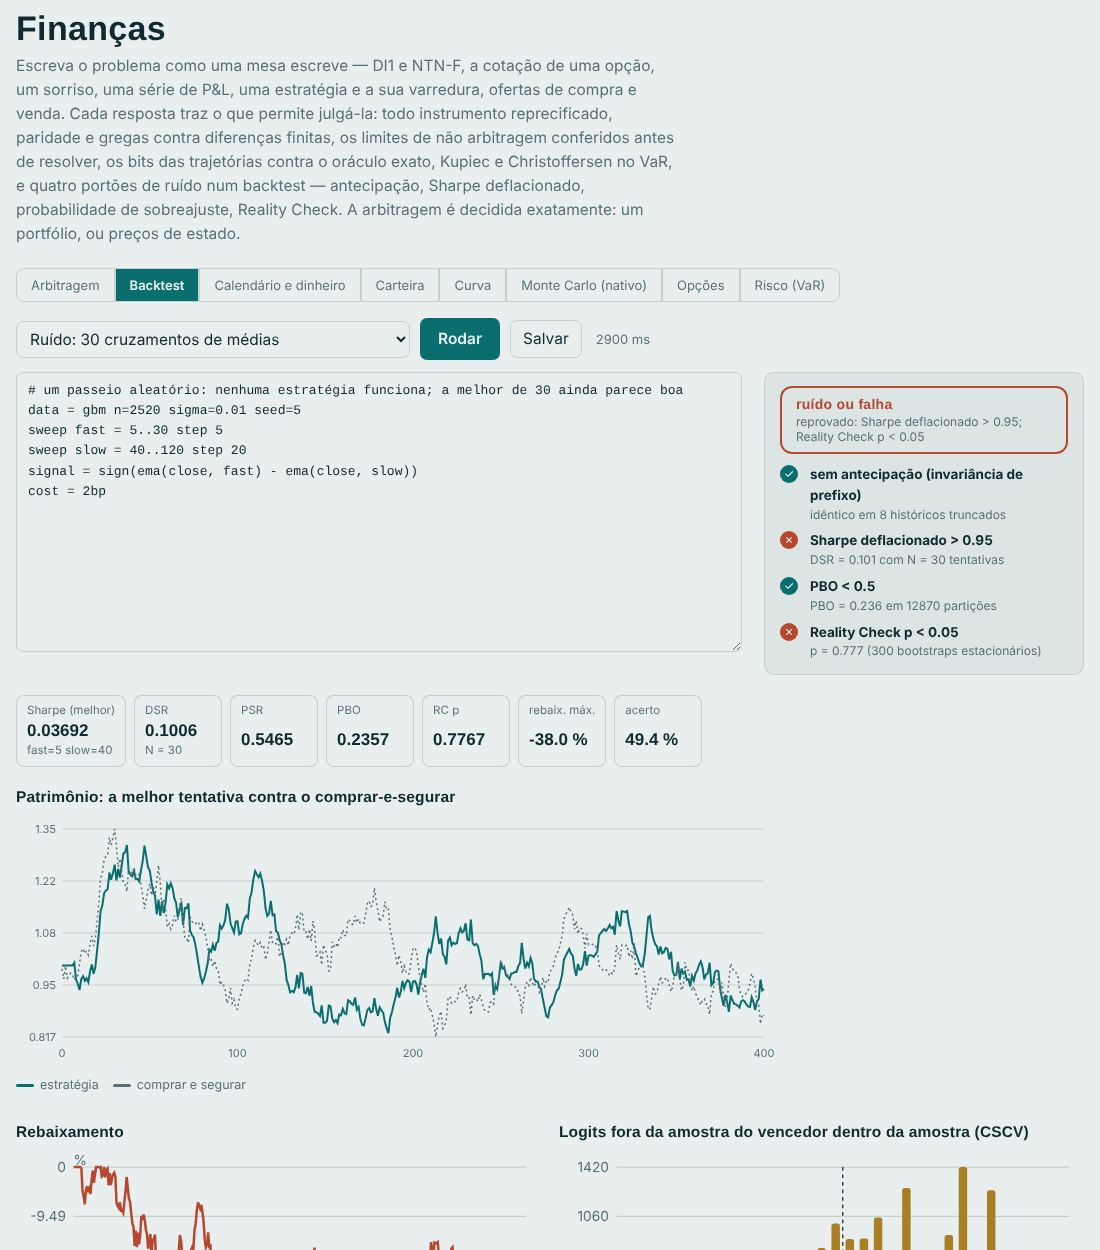
\includegraphics[width=0.82\textwidth]{figuras/console-financas-backtest.png}
\caption{Trinta cruzamentos de médias sobre ruído: o melhor parece bom, e os portões dizem que é ruído (DSR 0,10; \textit{Reality Check} $p = 0{,}78$).}
\label{fig:fin-backtest}
\end{figure}

% ----------------------------------------------------------------------------
\section{Arbitragem decidida exatamente}\label{sec:fin-arbitragem}

\begin{proposicao}[Lema de Farkas, forma de mercado]\label{prop:farkas}
Sejam $n$ ativos com pagamentos $X \in \mathbb{Q}^{n \times S}$ em $S$ estados e cotações $\mathrm{bid}_i \leq \mathrm{ask}_i$. Exatamente uma das alternativas vale:
\begin{enumerate}
  \item existe um portfólio --- compras $b \geq 0$ ao \textit{ask} e vendas $s \geq 0$ ao \textit{bid} --- com custo $\mathrm{ask}^\top b - \mathrm{bid}^\top s \leq 0$, pagamento $X^\top(b - s) \geq 0$ em todo estado, e pelo menos uma das desigualdades estrita;
  \item existem preços de estado $\psi \in \mathbb{Q}^S$, $\psi > 0$, com $\mathrm{bid}_i \leq (X\psi)_i \leq \mathrm{ask}_i$ para todo $i$.
\end{enumerate}
\end{proposicao}

É o teorema fundamental da precificação \cite{harrison1979,jouini1995} visto como teorema da alternativa \cite{farkas1902}. O \vapor{} acha os dois lados com um \textbf{simplex racional exato} (duas fases, regra de Bland contra ciclagem) e devolve o objeto que prova a alternativa encontrada, conferido \emph{só por multiplicação} de racionais:
\begin{itemize}
  \item uma arbitragem: o portfólio, o custo e o pagamento em cada estado. No exemplo da \textit{call} mal precificada, vender um título, comprar 1/90 da ação e vender 1/60 da \textit{call} recebe 1/15 hoje e paga 0 nos dois estados;
  \item ausência de arbitragem: o vetor $\psi > 0$ --- $(1/2,\, 9/20)$ no binomial do exemplo.
\end{itemize}

\begin{mestrado}
\textbf{Por que racionais.} Em ponto flutuante, a decisão entre as duas alternativas é instável na fronteira: um custo de $-10^{-17}$ é arbitragem ou erro de arredondamento? Em racionais, a resposta é exata, e o certificado é conferido por quem quiser com aritmética de inteiros. O custo é que coeficientes irracionais (como $e^{-rT}$) entram arredondados a 15 casas --- e a resposta diz isso. O mesmo simplex racional, com certificados dual, de Farkas e de raio ilimitado, resolve qualquer programa linear na mesa de lógica (\code{maximize}/\code{minimize}), fechando um item da lista de pendências da rodada 0.12.
\end{mestrado}

\paragraph{\textit{Calls} entre \textit{strikes}.} Para cotações de \textit{calls} num vencimento, os estados são 0, cada \textit{strike}, $2K_{\max}$ e a \emph{inclinação} além dele. Como o pagamento de qualquer combinação estática é linear por partes com vértices nos \textit{strikes}, conferir os vértices e a inclinação confere todo preço terminal: a decisão é completa para portfólios estáticos (\autoref{fig:fin-arb}). Câmbio: todos os ciclos simples de até cinco conversões, com o produto das taxas em racionais.

\begin{figure}[htbp]
\centering
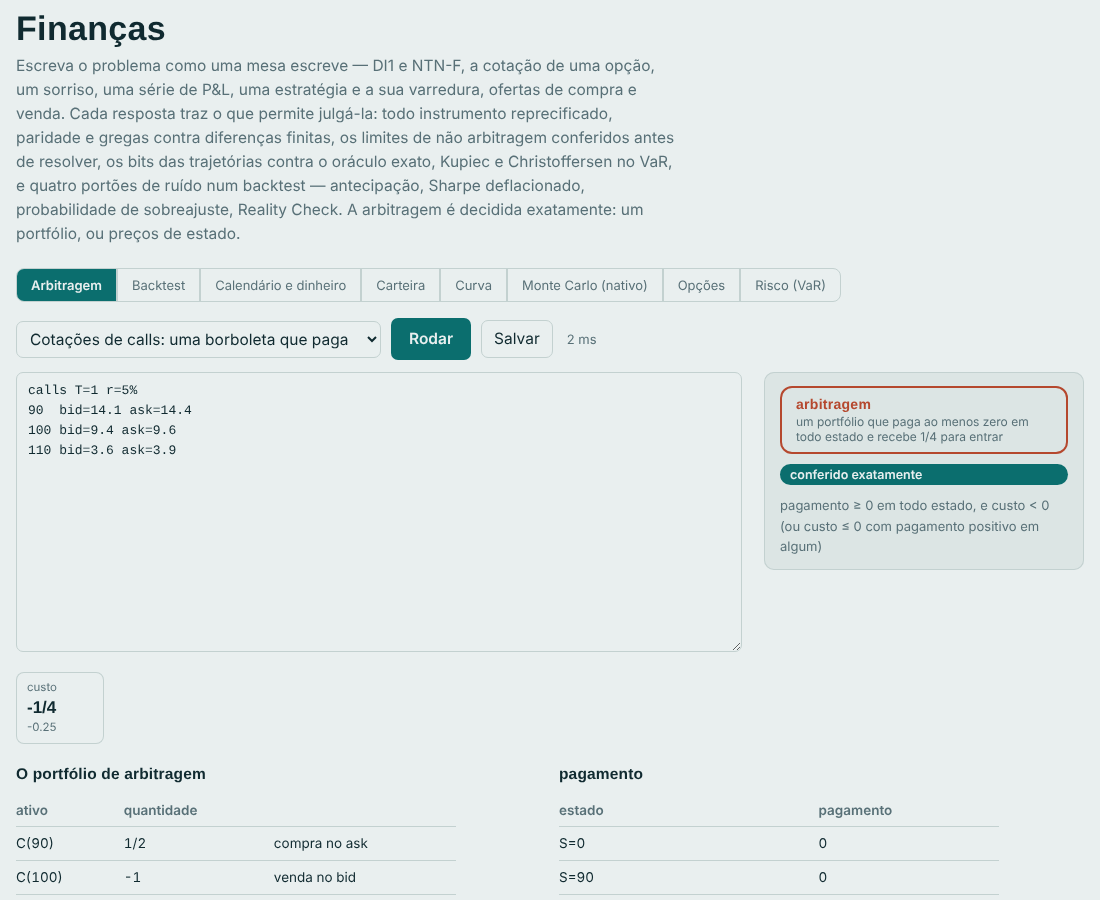
\includegraphics[width=0.82\textwidth]{figuras/console-financas-arbitragem.png}
\caption{Cotações de \textit{calls} com uma borboleta que paga: o portfólio de arbitragem, o custo exato e o pagamento em cada vértice.}
\label{fig:fin-arb}
\end{figure}

\paragraph{Humano ou IA no loop.} A ferramenta MCP \code{arbitrage\_check} recebe a \emph{proposta} de qualquer um --- um portfólio que alguém diz ser arbitragem, ou preços de estado que alguém diz provarem que não há --- e só a aritmética exata decide. O controle do teste: ``compre a ação e venda a \textit{call}'' paga nos dois estados mas custa 86,5 --- não é arbitragem, e a mesa diz por quê.

% ----------------------------------------------------------------------------
\section{O livro de ofertas como objeto verificável}\label{sec:fin-livro}

O motor de casamento implementa prioridade preço--tempo; ordens limitadas e a mercado; validades GTC, IOC e FOK; \textit{post-only}; cancelamento; alteração (reduzir a quantidade no mesmo preço mantém a prioridade; qualquer outra mudança é cancelar e substituir); prevenção de autonegociação; e \textit{kill switch} por dono. Preços são \textit{ticks} inteiros e quantidades são inteiras: nada arredonda. O motor é uma \textbf{função pura} $(\text{livro}, \text{evento}) \mapsto (\text{livro}', \text{relatórios})$.

\paragraph{Diário encadeado.} Cada entrada é $h_i = \mathrm{SHA256}(h_{i-1} \Vert \mathrm{CBOR}(\text{evento}_i, \text{relatórios}_i))$; a sessão fecha com uma raiz de Merkle sobre as entradas (folhas RFC~6962), e uma prova de inclusão mostra que um negócio pertence à sessão sem revelar os outros --- o que um regulador ou um cliente pede sem acesso ao livro inteiro.

\paragraph{O juiz independente.} O verificador (\code{Book.Check}) não compartilha nada com o motor além da especificação: o livro é uma lista, a prioridade é uma ordenação por (preço, tempo), cada casamento varre a lista. Do diário sozinho, ele refaz a cadeia de \textit{hashes}, \emph{reexecuta cada evento no motor ingênuo e exige os mesmos relatórios}, e confere nove invariantes (\autoref{fig:fin-juiz}).

\begin{figure}[htbp]
\centering
\begin{tikzpicture}[node distance=5mm and 6mm, font=\footnotesize]
\node[box] (ev) {eventos\\(texto, FIX)};
\node[box, right=of ev] (eng) {motor\\(mapas ordenados,\\filas por preço)};
\node[box, right=of eng] (j) {diário\\$h_i = H(h_{i-1} \Vert e_i \Vert r_i)$};
\node[dark, right=of j] (m) {raiz de\\Merkle};
\node[acc, below=10mm of j] (chk) {juiz ingênuo\\(lista + ordenação)};
\node[acc, left=of chk] (inv) {9 invariantes\\(não executam nada)};
\node[acc, right=of chk] (itch) {feed ITCH\\$\to$ livro reconstruído};
\draw[arr] (ev) -- (eng); \draw[arr] (eng) -- (j); \draw[arr] (j) -- (m);
\draw[carr] (j) -- node[lbl, right] {refaz} (chk); \draw[carr] (j.south west) -- (inv.north); \draw[carr] (j.south east) -- (itch.north);
\end{tikzpicture}
\caption{O livro de ofertas e os seus três verificadores independentes: o motor ingênuo, os invariantes e o feed de mercado.}
\label{fig:fin-juiz}
\end{figure}

Os invariantes são: preço do negócio igual ao do \textit{maker} e dentro do limite do agressor; o \textit{maker} é o primeiro na prioridade naquele instante; quantidades conservadas (executado + repousado + cancelado = ordenado); livro nunca cruzado; FOK tudo ou nada; IOC e ordem a mercado nunca repousam; \textit{post-only} nunca agride; nenhum negócio entre ordens do mesmo dono sob prevenção; e cadeia íntegra.

\paragraph{O defeito que o juiz achou.} O \textit{fuzzing} diferencial roda 6\,000 eventos aleatórios por política de prevenção, comparando motor e juiz. Na primeira rodada, o juiz apontou \code{:fok\_partial}: uma ordem \textbf{FOK a mercado} virava IOC nos \emph{dois} motores --- a mesma leitura errada da especificação, escrita duas vezes. A reexecução não a pegou, porque os dois motores concordavam; só o invariante, que não executa nada, viu. O defeito foi corrigido nos dois motores e o invariante ficou. O episódio ilustra por que o juiz tem duas camadas de natureza diferente: reexecução (pega divergência de implementação) e invariantes (pegam erro de especificação comum).

\paragraph{Adulteração.} Um preço trocado num diário quebra a cadeia. O mesmo negócio forjado \emph{com o \textit{hash} recalculado} --- uma mentira coerente --- passa na cadeia e cai na reexecução.

\paragraph{Desempenho, honestamente.} Cerca de 8,5~$\mu$s por evento na mediana (p99 de cerca de 100~$\mu$s), \emph{incluindo} o SHA-256 e a codificação canônica de cada entrada; o juiz reexecuta 12\,500 eventos em cerca de 150~ms. A BEAM é tempo real brando: esses números servem a um casamento de mesa, a um internalizador, a um simulador de \textit{backtest} --- não a uma bolsa de nanossegundos.

\begin{figure}[htbp]
\centering
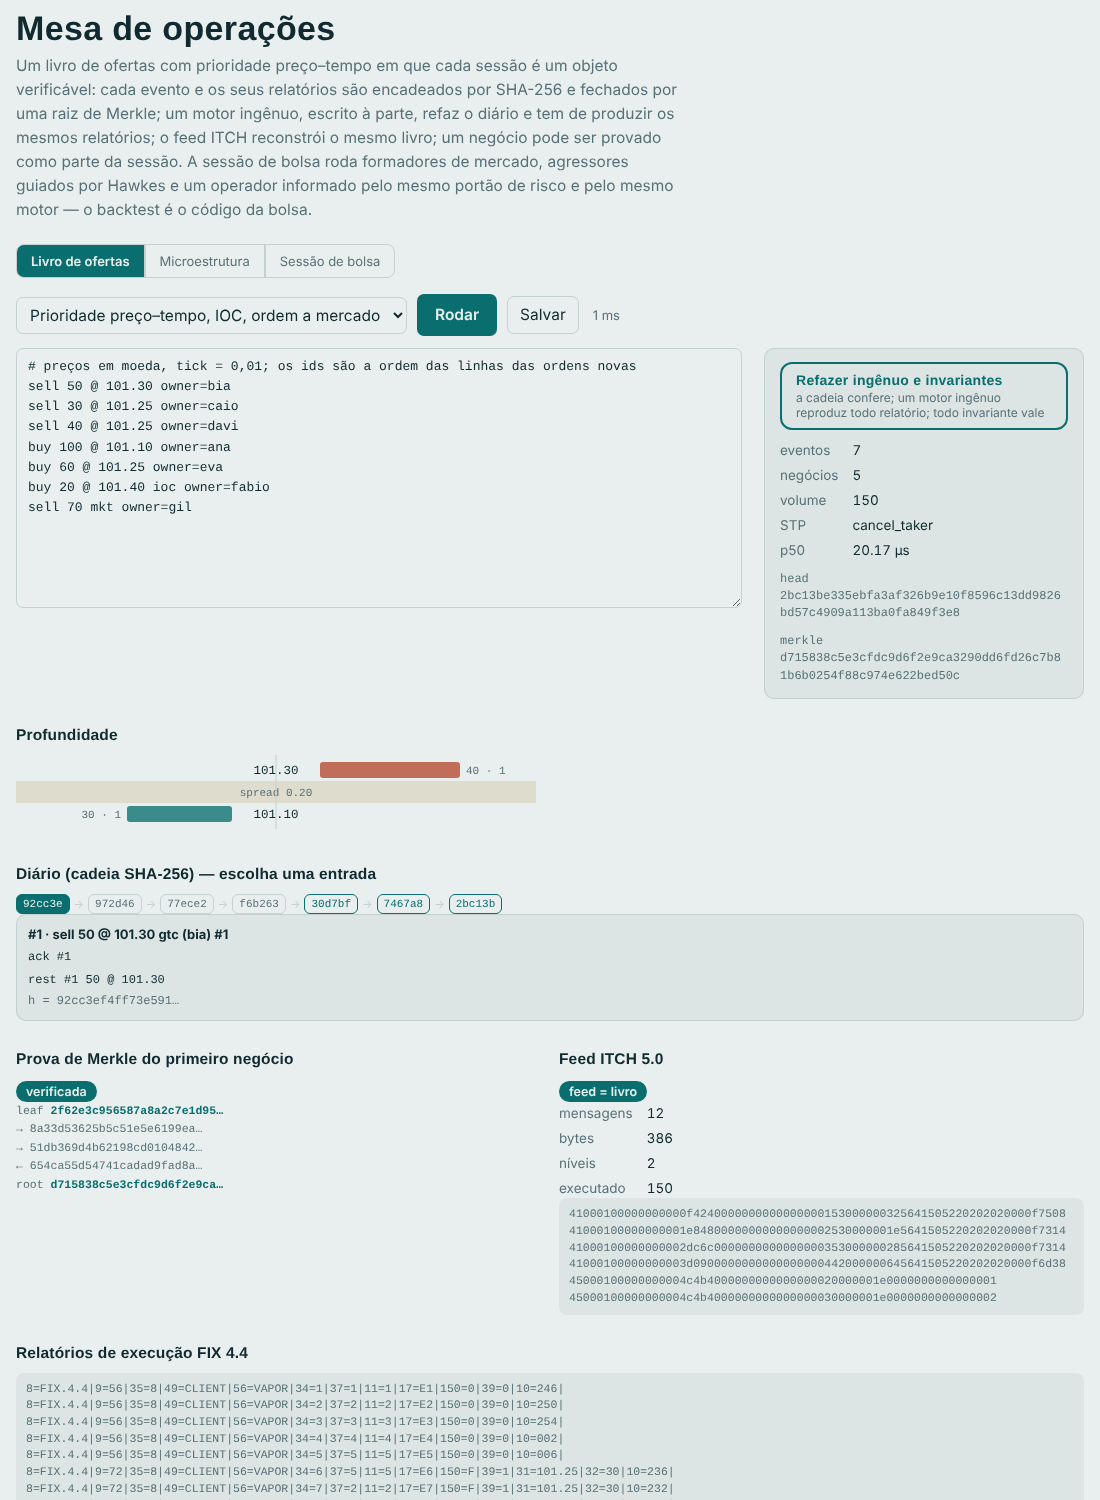
\includegraphics[width=0.82\textwidth]{figuras/console-mesa-livro.png}
\caption{O livro de ofertas no console: profundidade, o diário encadeado (cada entrada selecionável), a prova de Merkle do primeiro negócio, o feed ITCH e os relatórios FIX.}
\label{fig:fin-livro}
\end{figure}

% ----------------------------------------------------------------------------
\section{Protocolos e risco pré-negociação}\label{sec:fin-protocolos}

\paragraph{ITCH 5.0.} Codificador e decodificador das mensagens S, R, A, F, E, C, X, D, U e P da especificação da Nasdaq \cite{itch50}, com os comprimentos exatos (12 a 44 bytes, \textit{big-endian}, preço com 4 casas implícitas, \textit{timestamp} de 6 bytes em nanossegundos). A sessão gera o feed que uma bolsa publicaria, e \code{rebuild/1} reconstrói o livro \emph{só a partir do feed} --- que tem de ser igual ao do motor, nível a nível, e com o mesmo volume executado: um terceiro certificado independente (o feed só vê o que repousa; o motor vê tudo).

\paragraph{FIX 4.4.} Mensagens tag=valor com \textit{BodyLength} (9) e \textit{CheckSum} (10) conferidos na leitura e calculados na escrita --- iguais ao \code{simplefix} byte a byte \cite{fix44}. \textit{NewOrderSingle}, \textit{OrderCancelRequest} e \textit{OrderCancelReplaceRequest} viram eventos do livro; os relatórios viram \textit{ExecutionReports} com numeração própria.

\paragraph{Risco pré-negociação.} O que a Regra 15c3-5 da SEC \cite{sec15c35} e o RTS~6 da MiFID~II \cite{rts6} pedem a quem tem acesso ao mercado --- \emph{e que possa mostrar que tinha}: quantidade máxima (``dedo gordo''), nocional máximo, colar de preço contra a referência, posição máxima no pior caso (executado + ordens abertas daquele lado + esta), taxa de mensagens numa janela e \textit{kill switch}. Uma recusa nunca chega ao livro e \emph{entra no diário} com a causa. O verificador refaz posições, ordens abertas, referências e contagens a partir do diário e confere que nenhuma ordem aceita violou um limite \emph{e que toda recusa teve a causa dita}. O controle atribui a uma recusa por quantidade a causa ``colar de preço'', e é pego.

% ----------------------------------------------------------------------------
\section{Microestrutura, cada modelo com a medida que diz se serve}\label{sec:fin-micro}

\paragraph{Hawkes.} Chegadas que se excitam, com intensidade $\lambda(t) = \mu + \sum_{t_i < t} \alpha e^{-\beta(t - t_i)}$ \cite{hawkes1971,bacry2015}: simulação por \textit{thinning} de \citeonline{ogata1981}, máxima verossimilhança pela recursão $O(n)$, e o \textbf{teste de reescala do tempo}: sob o modelo certo, os incrementos do compensador $\Lambda(t_i) - \Lambda(t_{i-1})$ são Exp(1), julgados por Kolmogorov--Smirnov. Plantado $(\mu, \alpha, \beta) = (1;\, 0{,}6;\, 1{,}5)$, ajustado $(1{,}08;\, 0{,}61;\, 1{,}69)$, razão de ramificação $0{,}36$ (plantada $0{,}40$), KS $p = 0{,}73$. O controle --- um Poisson ajustado às mesmas chegadas --- tem $p = 1{,}7 \cdot 10^{-20}$ (\autoref{fig:fin-hawkes}).

\begin{figure}[htbp]
\centering
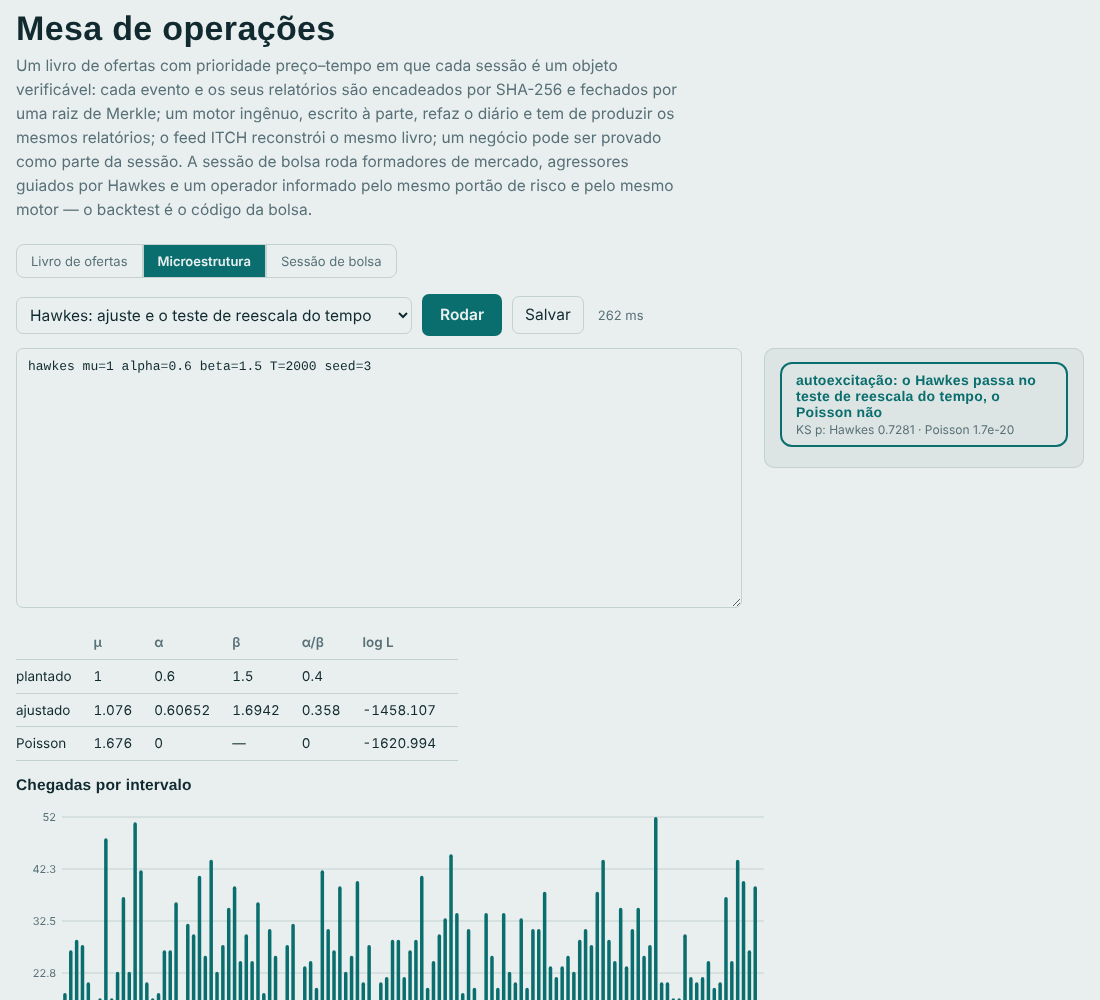
\includegraphics[width=0.78\textwidth]{figuras/console-mesa-hawkes.png}
\caption{Hawkes: os parâmetros plantados e ajustados, o Poisson como controle e o teste de reescala do tempo.}
\label{fig:fin-hawkes}
\end{figure}

\paragraph{Avellaneda--Stoikov.} O formador de mercado de \citeonline{avellaneda2008} cota em torno do preço de reserva $r = s - q\gamma\sigma^2(T - t)$ com \textit{spread} total $\gamma\sigma^2(T-t) + \frac{2}{\gamma}\ln(1 + \frac{\gamma}{k})$. A simulação do §4 do artigo ($s_0 = 100$, $T = 1$, $\sigma = 2$, $dt = 0{,}005$, $k = 1{,}5$, $A = 140$, 1\,000 trajetórias, $\gamma = 0{,}1$) dá, daqui contra o artigo, $\sigma(\text{P\&L})$ de 6,44 / 5,89 para a estratégia de estoque e 13,57 / 13,43 para a simétrica. O \textit{spread} médio daqui (1,49) inclui o termo $\gamma\sigma^2(T-t)$ que a tabela do artigo parece omitir (1,29 é só o segundo termo) --- dito, não escondido.

\paragraph{Almgren--Chriss.} A trajetória ótima de liquidação $x_j = X \sinh(\kappa(T - t_j))/\sinh(\kappa T)$ \cite{almgren2000}, com $\kappa$ da relação discreta $\cosh(\kappa\tau) = 1 + \tilde\kappa^2\tau^2/2$, é \emph{certificada} resolvendo o mesmo problema de média--variância numericamente (um sistema tridiagonal): diferença relativa $10^{-16}$.

% ----------------------------------------------------------------------------
\section{Uma sessão de bolsa que se audita}\label{sec:fin-sessao}

A sessão de bolsa junta tudo: formadores de mercado cotando \textit{post-only} pela regra de Avellaneda--Stoikov em torno do preço público do passo anterior; agressores de ruído cujas chegadas seguem um Hawkes exato em tempo contínuo; um operador informado que conhece o fundamental e agride quando o livro se afasta dele. Toda ordem passa pelo mesmo portão pré-negociação e pelo mesmo motor que uma implantação usaria --- \textbf{o \textit{backtest} é o código da bolsa}, não um modelo dela.

A sessão devolve a própria auditoria (\autoref{fig:fin-sessao}): o diário conferido pelo motor ingênuo, os limites conferidos a partir do diário, o feed ITCH reconstruindo o mesmo livro, e a mesma semente reproduzindo a mesma cabeça de \textit{hash}. E a microestrutura medida na fita recupera o que foi plantado: o ajuste de Hawkes das chegadas acha a autoexcitação (ramificação 0,37 contra 0,40; o Poisson rejeitado), e o \textit{spread} de Roll (5,66) fica próximo do cotado (5,85).

\begin{figure}[htbp]
\centering
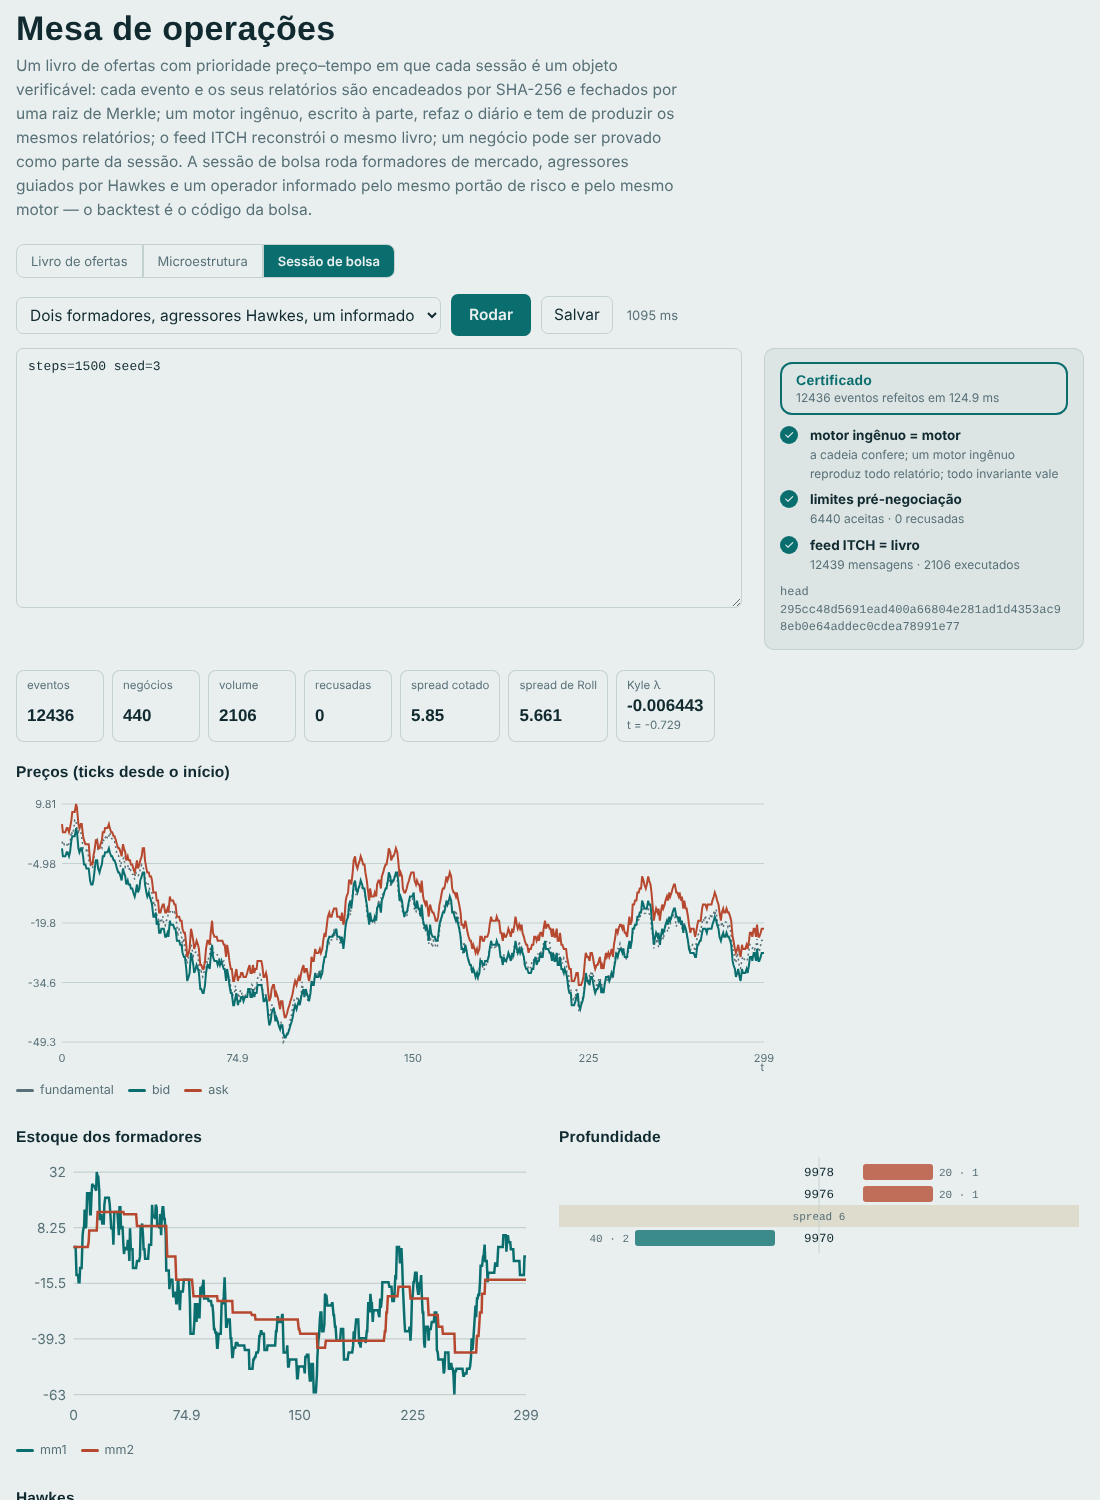
\includegraphics[width=0.82\textwidth]{figuras/console-mesa-sessao.png}
\caption{Uma sessão de 1\,500 passos: 12\,436 eventos refeitos pelo motor ingênuo, limites pré-negociação conferidos, feed ITCH igual ao livro; preços, estoques dos formadores e profundidade.}
\label{fig:fin-sessao}
\end{figure}

\begin{doutorado}
\textbf{Simuladores de mercado verificáveis.} Simuladores baseados em agentes \cite{byrd2020} são usados para treinar e avaliar estratégias, mas o seu motor de casamento raramente é o de uma bolsa real, e os resultados raramente são reproduzíveis entre versões. A sessão do \vapor{} mostra que é possível ter as duas coisas --- o motor de produção e a reprodutibilidade por \textit{hash} ---, mas numa escala de microssegundos. Ficam em aberto: (i) se o motor, compilado como programa canônico ou escrito no worker, pode chegar à escala de nanossegundos mantendo o diário e o juiz fora do caminho crítico; (ii) como calibrar os agentes a dados reais de alta frequência de modo que a microestrutura medida (Hawkes, Roll, Kyle, assinatura da variância) seja um teste de aderência do simulador, e não só uma ilustração.
\end{doutorado}

% ----------------------------------------------------------------------------
\section{O que este capítulo não afirma}\label{sec:fin-limites}

\begin{itemize}
  \item \textbf{Latência de bolsa.} O motor roda na BEAM: microssegundos por evento com \textit{hash}, não nanossegundos. O que se afirma é a verificabilidade e a identidade entre \textit{backtest} e motor.
  \item \textbf{Dados reais.} Nenhum arquivo ITCH da Nasdaq e nenhuma curva da ANBIMA foram usados; os preços dos exemplos são ilustrativos. Os formatos são os das especificações e as convenções as publicadas; os oráculos são o QuantLib, o \code{simplefix}, o SciPy e o ngspice, não os dados.
  \item \textbf{Conselho de investimento.} Os portões dizem quando um \textit{backtest} é indistinguível de ruído; passar neles não torna uma estratégia lucrativa (custos reais, capacidade, mudança de regime).
  \item \textbf{Modelos completos de mercado.} Não há XVA, modelos de taxa de juros de vários fatores (Hull--White, LMM), volatilidade local ou estocástica calibrada a uma superfície inteira, nem crédito.
\end{itemize}

% ============================================================================
\chapter{A bancada aberta: a rodada 0.14}\label{cap:bancada}
% ============================================================================

As rodadas 0.11 e 0.12 aplicaram a separação ``uma busca propõe, um verificador decide'' a domínios escolhidos: redes de ordenação, geometria, engenharia, lógica, tabuleiros. Cada domínio era uma mesa com o seu formato de entrada e os seus exemplos. A crítica que abriu a rodada 0.14 foi direta: o módulo de ciência apresentava \emph{problemas já resolvidos}; as cenas aceitavam só ações pré-determinadas; o sistema era expositivo. Este capítulo descreve a resposta --- trocar \emph{N mesas} por \textbf{uma linguagem, uma fornalha e uma pedra de toque} --- e o que as verificações com controle disseram dela.

\begin{graduacao}
\textbf{Glossário mínimo.} Um \emph{espaço de busca} é o conjunto de candidatos possíveis (permutações, subconjuntos, grafos\ldots). Uma \emph{meta-heurística} (recozimento simulado, algoritmo evolutivo) explora esse espaço sem garantia de ótimo. Um \emph{processo gaussiano} é um modelo estatístico de uma função desconhecida, usado para escolher o próximo ponto a medir quando cada medida é cara. Um \emph{holdout} é um conjunto de dados reservado que a busca não vê, usado para descobrir se o vencedor só venceu por acaso.
\end{graduacao}

% ----------------------------------------------------------------------------
\section{Escrutínio do pedido}\label{sec:banc-escrutinio}

O pedido pedia ``uma grande coletânea'' de buscadores famosos, generalizados. Tomado ao pé da letra, isso produziria $N$ ferramentas estreitas com $N$ formatos --- exatamente a falta de liberdade criticada. O denominador comum desses buscadores é um laço de três passos: \emph{proponha} um candidato, \emph{avalie-o} com um verificador, \emph{guarde} o resultado com a prova. O produto, então, é o caso geral; os casos famosos viram \emph{exemplos de partida} escritos na mesma linguagem que o usuário usa (régua de Golomb, Ramsey, a conjectura de Euler, redes de ordenação, caixeiro-viajante, portfólios, hiperparâmetros, exemplos adversariais, regras de \textit{trading}, fórmulas). Os nomes do sistema seguem a metáfora do laboratório alquímico --- \emph{Alembic}, \emph{Athanor}, \emph{Touchstone}, \emph{Crucible}, \emph{Assay} --- e nenhum nome de produto de terceiros é usado.

Dois riscos do pedido foram tratados como requisitos. \textbf{Entrada aberta} sem sanitização é uma porta de ataque; sanitização por lista de palavras é frágil. \textbf{``AI em tudo''} sem verificação é autoridade sem prova. As duas seções seguintes mostram as respostas.

% ----------------------------------------------------------------------------
\section{Alembic: uma linguagem pura e saneada}\label{sec:banc-alembic}

Alembic é uma linguagem de expressões pura: inteiros de tamanho arbitrário, listas, tuplas, mapas, compreensões, \textit{lambdas}, \textit{pipes} e cerca de 120 funções embutidas, sem E/S, sem relógio e sem aleatoriedade fora de \code{noise} e \code{hash}, que são determinísticas. Um programa é, portanto, uma função do seu texto --- o que torna reprodutível o diário de toda busca que o use.

A sanitização é feita pela \emph{semântica}, não por filtros (\autoref{tab:banc-limites}): todo passo paga combustível; tamanhos têm teto; a avaliação roda num processo com teto de memória que a máquina virtual mata; identificadores nunca viram átomos (a tabela de átomos da BEAM não é coletada); dados são lidos por um leitor que recusa código; e, no navegador, as expressões das cenas são uma árvore JSON \emph{interpretada}, nunca avaliada como JavaScript. A mesma análise achou um vazamento antigo: \code{Vapor.Expr.compile/2} criava um módulo BEAM (e um átomo) por expressão nova; agora há um teto, e o excedente é interpretado sem criar átomo algum.

\begin{table}[htbp]
\centering
\caption{Os limites da Alembic e o teste que tenta quebrar cada um}\label{tab:banc-limites}
\small
\begin{tabularx}{\textwidth}{@{}l>{\raggedright\arraybackslash}X>{\raggedright\arraybackslash}X@{}}
\toprule
\textbf{risco} & \textbf{defesa} & \textbf{teste}\\
\midrule
laço infinito & combustível em toda chamada e iteração & recursão sem fim e \code{fold} gigante recusados\\
números enormes & inteiros até 65\,536 bits & $2^{10^8}$ recusado\\
memória & processo com \code{max\_heap\_size} & bomba de memória morta sob 16 MB; o chamador vive\\
átomos & identificadores ficam binários & 2\,000 nomes novos: 0 átomos\\
código como dado & leitor de literais & \code{f(1)} e compreensões recusados\\
injeção no navegador & árvore interpretada & funções não numéricas recusadas\\
\bottomrule
\end{tabularx}
\end{table}

% ----------------------------------------------------------------------------
\section{Athanor e Touchstone}\label{sec:banc-athanor}

Um problema Athanor é um programa Alembic com nomes reservados: \code{space} (dez construtores: \code{bits}, \code{ints}, \code{reals}, \code{perm}, \code{subset}, \code{subsets}, \code{seq}, \code{graph}, \code{partition} e \code{program}, árvores de expressão), um objetivo (\code{minimize}, \code{maximize}) ou uma afirmação (\code{claim}), e opcionalmente \code{violation} (a distância até a validade, que ordena os inválidos e deixa a busca subir até eles), \code{holdout}, \code{describe} (para um arquivo MAP-Elites), \code{neighbor} e \code{measured}.

A fornalha reparte o orçamento entre estratégias --- exaustiva retomável, aleatória, recozimento, evolução, CMA-ES, otimização bayesiana com processo gaussiano Matérn-5/2, \emph{mente} (um modelo de linguagem) e \emph{humano} --- por um bandido UCB descontado ($\gamma = 0{,}97$). A primeira versão, com UCB simples, gastava demais na aleatória; sem a aleatória, perdia nos problemas rugosos; o desconto resolveu os dois. Toda corrida termina com três objetos que a tornam julgável:
\begin{enumerate}
  \item o \textbf{controle}: o mesmo orçamento gasto em amostras uniformes; se o acaso nunca alcança o melhor, a regra de três dá o limite superior da chance por amostra;
  \item o \textbf{\textit{holdout}}: os finalistas reavaliados num objetivo não visto, com a correlação de postos de Spearman e o máximo esperado do ruído, $\sqrt{2 \ln N}$;
  \item o \textbf{diário}: uma cadeia SHA-256 sobre a codificação canônica de cada avaliação, cuja raiz depende só do texto e da semente.
\end{enumerate}

A \textbf{Touchstone} reconfere um certificado sem confiar na busca: reavalia o candidato, confere pertença e valor; com \code{full}, refaz a enumeração; com \code{replay}, refaz a corrida e compara a raiz do diário. ``Provado'' significa exatamente \emph{enumeração completa de um espaço finito}, e o certificado diz o tamanho.

\paragraph{Humano e modelo no laço.} Uma sessão corre sob supervisão; a pessoa observa, propõe candidatos, fixa e bane finalistas, estende o orçamento ou fornece medidas de um objetivo externo (um experimento, um treino). Um modelo de linguagem pode \emph{formalizar} um problema descrito em palavras --- o rascunho é compilado, reparado até três vezes com o erro do compilador e devolvido com uma \emph{retrotradução} para a pessoa conferir --- e pode \emph{propor} candidatos. As propostas, venham de onde vierem, entram pela mesma porta e são julgadas pelo mesmo verificador. O modelo nunca decide.

% ----------------------------------------------------------------------------
\section{Crucible: evidência sem gabarito}\label{sec:banc-crucible}

Os experimentos científicos das rodadas anteriores comparavam a saída com uma resposta conhecida --- útil como calibração, inútil para quem traz um sistema novo, cuja resposta ninguém conhece. O Crucible aceita o sistema do usuário (EDOs, potenciais, hamiltonianos, reações, sequências, moléculas, dados) e responde com evidência que \emph{não precisa de gabarito}: a ordem de convergência observada por Richardson; teoremas que valem para qualquer entrada (virial, Ehrenfest, trabalho--energia); dois métodos independentes que precisam concordar; e controles que um método errado reprovaria.

O caso mais forte são as \textbf{leis de conservação provadas sobre $\mathbb{Q}$}. Para um campo vetorial polinomial, um candidato $I = \sum_k c_k m_k$ (monômios e, opcionalmente, logaritmos das variáveis) é conservado se e só se a derivada de Lie $\sum_i f_i \,\partial I/\partial x_i$ se anula identicamente; isso é um sistema linear nos $c_k$, resolvido exatamente em racionais. Para a epidemia SIR, o método acha $S + I + R$ e $3S + 3I - \ln S$, ambos provados, e mostra que sobrevivem a perturbar cada coeficiente em 1\,\% (são estruturais). Na verificação com controle (\autoref{tab:qualidade14}), seis hamiltonianos cúbicos aleatórios têm o seu $H$ redescoberto e provado, e seis sistemas dissipativos aleatórios não recebem lei nenhuma.

% ----------------------------------------------------------------------------
\section{Assay: essa diferença é real?}\label{sec:banc-assay}

Voltando às raízes do projeto em pesquisa de IA, o Assay ataca a dor mais comum do campo, que não é treinar, mas \emph{decidir se uma diferença de avaliação é real}: comparação pareada com \textit{bootstrap}, permutação por troca de sinal e McNemar exato, junto do efeito mínimo detectável; \textit{leaderboards} com empates declarados; calibração medida contra o seu próprio piso (o ECE que um modelo perfeitamente calibrado teria com aquelas confianças e aquele $n$); concordância de anotadores (Krippendorff, Fleiss, Cohen); viés de posição de juízes; contaminação por 13-gramas; deduplicação por MinHash verificada por Jaccard exato; e leis de escala na forma de Hoffmann, que precisam \emph{prever as maiores corridas sem tê-las visto}.

O controle da lei de escala --- as mesmas corridas com as perdas embaralhadas --- achou um defeito real: sem estrutura nos dados, os parâmetros em escala logarítmica cresciam até estourar a exponencial. O ajuste agora permanece finito, e o \textit{holdout} reporta erro de 33\,\% contra 0,3\,\% com os dados verdadeiros: a lei não prevê nada, que é a resposta certa.

% ----------------------------------------------------------------------------
\section{Interfaces: o terminal primeiro}\label{sec:banc-interfaces}

Toda capacidade da bancada está disponível na linha de comando (\code{bin/vapor}), na filosofia Unix: leitura da entrada padrão, JSON quando a saída é um \textit{pipe}, e códigos de saída com significado (0 positivo, 1 negativo --- refutado, não achado, verificação falhou, ruído ---, 2 uso, 3 entrada inválida, 4 falha). O console web, a TUI e as 20 ferramentas MCP chamam as mesmas funções. O console ganhou uma identidade visual própria em que o ornamento coincide com a informação: a \emph{fornalha} é o gráfico ao vivo da busca (faíscas por avaliação, a linha do melhor, a linha tracejada do controle, a partilha do portfólio) e a \emph{pedra de toque} é o veredito, um risco de ouro por verificação aprovada e de chumbo pela reprovada (\autoref{fig:banc-console}). As cenas passaram a ser documentos editados por operações de texto, com expressões por quadro e direção por modelo.

\begin{figure}[htbp]
\centering
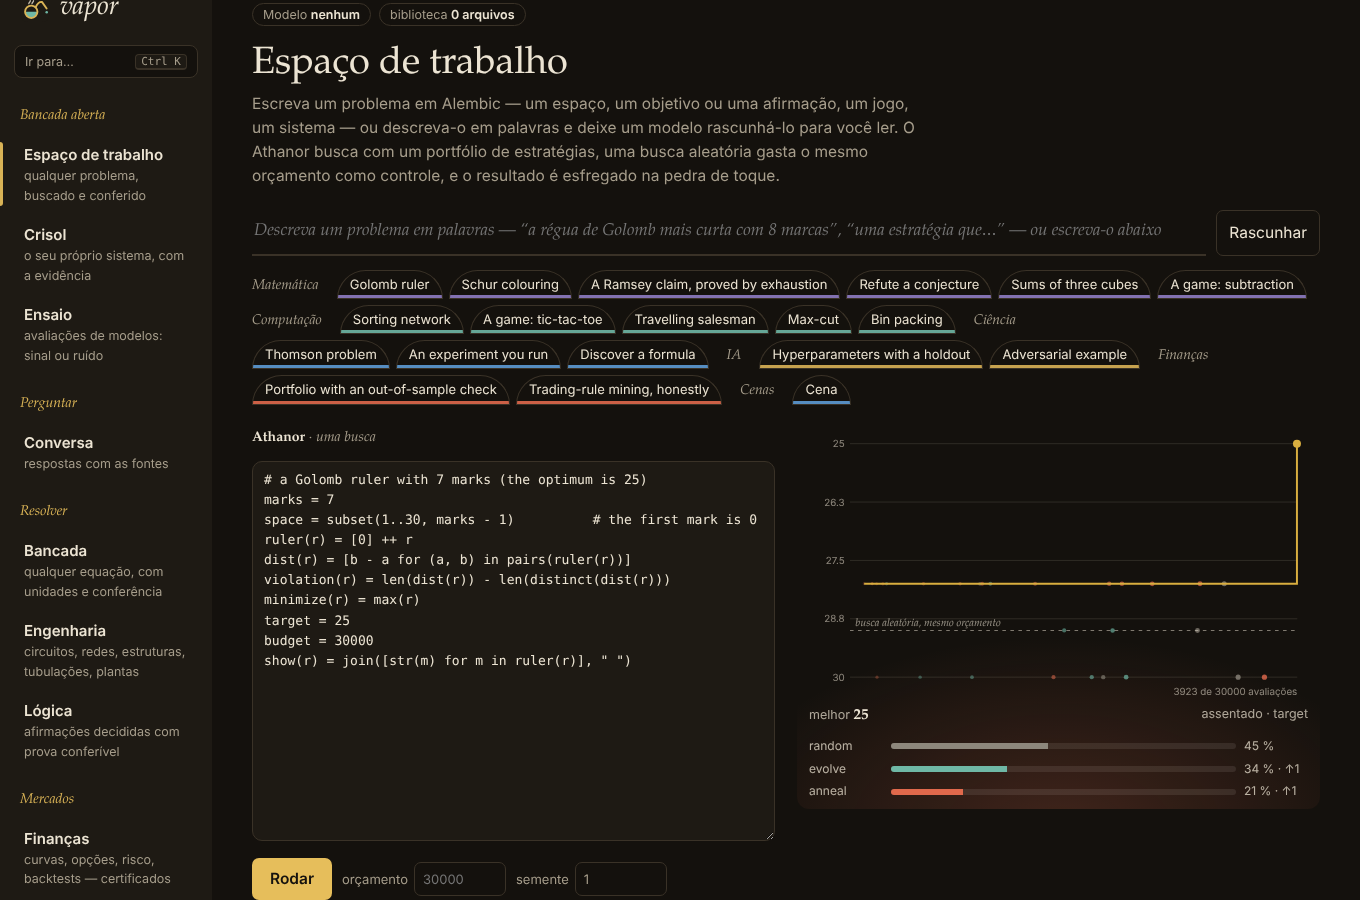
\includegraphics[width=0.9\textwidth]{../docs/img/bancada-athanor-escuro.png}
\caption{O espaço de trabalho: a régua de Golomb de 7 marcas achada no ótimo (25); a linha tracejada é a busca aleatória com o mesmo orçamento, que não passou de 28; abaixo, a partilha do portfólio.}
\label{fig:banc-console}
\end{figure}

% ----------------------------------------------------------------------------
\section{O que este capítulo não afirma}\label{sec:banc-limites}

\begin{itemize}
  \item Que ``provado'' signifique mais que enumeração completa de um espaço finito; espaços infinitos dão evidência, e o certificado diz qual.
  \item Que a fornalha seja competitiva com resolvedores especializados (SAT, MIP) nos seus domínios --- as mesas exatas de lógica e de programação linear continuam existindo.
  \item Que o rascunho de um modelo esteja certo: a retrotradução existe para que a pessoa confira.
  \item Química além de STO-3G de camada fechada com H e He.
\end{itemize}

% ============================================================================
\chapter{Avaliação}\label{cap:avaliacao}
% ============================================================================

Este capítulo responde a uma pergunta: \emph{como se sabe que o que os capítulos anteriores afirmam é verdade?} A resposta tem três partes --- oráculos externos, controles e propriedades bit a bit ---, e termina com as ameaças à validade, isto é, com as razões pelas quais a resposta pode estar errada.

% ----------------------------------------------------------------------------
\section{Metodologia}\label{sec:aval-metodo}

\paragraph{Três tipos de evidência.} (1) \textbf{Oráculos externos}: uma implementação independente, de terceiros, amplamente usada, contra a qual o resultado do \vapor{} é comparado --- com igualdade bit a bit quando a semântica é a mesma, com tolerância declarada quando não é. (2) \textbf{Controles}: para cada verificação, o valor que uma implementação quebrada, ingênua ou trapaceira produziria; a verificação só é aceita se o controle cai do outro lado do limiar. (3) \textbf{Propriedades}: igualdades bit a bit entre substratos, \textit{threads}, lotes e réplicas, que não precisam de oráculo porque comparam o sistema consigo mesmo sob transformações que não deveriam mudar nada.

\paragraph{Oráculos.} A \autoref{tab:oraculos} lista os oráculos por domínio. Todos aparecem só nos testes; o produto não depende de nenhum.

\begin{table}[htbp]
\centering
\caption{Oráculos externos usados nos testes}\label{tab:oraculos}
\small
\begin{tabularx}{\textwidth}{@{}lX@{}}
\toprule
\textbf{domínio} & \textbf{oráculo e critério}\\
\midrule
codificação de instruções & GNU binutils (x86 com EVEX, AArch64, \code{rv64gcv}); \code{spirv-val} --- toda instrução emitida\\
execução cruzada & QEMU \textit{user} (aarch64, riscv64, VLEN 128/256/512); Mesa lavapipe (Vulkan)\\
aritmética & \code{fmaf}, \code{+}, \code{*} do \textit{hardware} --- 800\,000 operações, bit a bit; \code{mpmath} para funções\\
modelos & \code{transformers}, \code{diffusers} (PyTorch) --- logits, \textit{hidden states}, imagens\\
formatos & \code{gguf-py}, \code{llama.cpp}, libjpeg, libtiff, jbig2dec, \code{jinja2}, \code{cbor2}\\
engenharia & ngspice (circuitos, inclusive MOSFET nível 1 e Ebers--Moll); soluções analíticas\\
finanças & QuantLib 1.43 (calendários, bases, curvas, BSM, Leisen--Reimer, Heston); \code{simplefix} (FIX); SciPy; Python \code{decimal}; artigos (Longstaff--Schwartz, Avellaneda--Stoikov, Gatheral--Jacquier)\\
protocolos & SDK oficial do MCP; cliente \code{openai}\\
\bottomrule
\end{tabularx}
\end{table}

\paragraph{Máquina.} Os números desta monografia foram medidos num Xeon de 2,1~GHz com 2 vCPUs e AVX-512, sem GPU física e sem contadores de desempenho, com Elixir 1.14/OTP~25 e Zig 0.16. O \autoref{ap:reproducao} lista os comandos.

% ----------------------------------------------------------------------------
\section{Testes}\label{sec:aval-testes}

A suíte é organizada em \emph{níveis}, cada um ligado à ferramenta externa de que depende; um nível sem a ferramenta presente é excluído e relatado como tal, nunca contado como aprovado. A \autoref{tab:testes} mostra a evolução por rodada.

\begin{table}[htbp]
\centering
\caption{Testes por rodada (execução completa de \code{mix test})}\label{tab:testes}
\small
\begin{tabular}{@{}lrrl@{}}
\toprule
\textbf{rodada} & \textbf{executados} & \textbf{falhas} & \textbf{observação}\\
\midrule
0.5 & 343 & 0 & 32 excluídos por ferramenta ausente\\
0.6 & 400 & 2 $\to$ 0 & uma violação real de arquitetura achada e corrigida\\
0.7 & 425 & 0 & \\
0.8 & 469 & 1 $\to$ 0 & teste antigo exigia recusar JBIG2, agora decodificado\\
0.9 & 501 & 0 & todos os níveis presentes, salvo 18\\
0.11 & 611 & 0 & \\
0.12 & 702 & 0 & 115 excluídos por ferramenta ausente na sessão\\
0.13 & \testesTreze & \falhasTreze & \obsTreze\\
0.14 & \testesQuatorze & \falhasQuatorze & \obsQuatorze\\
\bottomrule
\end{tabular}
\end{table}

Na rodada 0.13, a execução completa da suíte foi interrompida por um reinício da máquina virtual e não foi repetida; o que a tabela registra são os 108 testes dos oito arquivos que a rodada tocou (finanças, console de mercados, rodada 13, arquivos, MCP, engenharia, bancada e lógica), todos aprovados. Os demais módulos não mudaram desde a execução completa da 0.12. Os testes novos de finanças (41) usam o QuantLib, o SciPy e o \code{simplefix} como oráculos; os de transistores, o ngspice; os do console, um navegador sem cabeça que roda \emph{todo exemplo de todo painel} das duas mesas, em inglês e em português, e confere que nenhum rótulo ou frase em inglês sobra na versão em português.

Na rodada 0.14, os 87 testes dos oito arquivos da bancada aberta (Alembic, Athanor, Crucible, Assay, mente, operações de cena, espaço de trabalho de ponta a ponta e MCP) passaram, assim como o teste com o SDK oficial de MCP em Python, o de paridade do ruído em JavaScript e os dois testes de navegador sem cabeça das mesas antigas. Estes últimos acharam duas coisas: a ordem alfabética exigida na barra lateral, que o novo grupo ``Bancada aberta'' quebra de propósito (a ordem dele é a do trabalho: escrever, conferir, medir --- o teste passou a respeitar grupos marcados como fixos); e um defeito real e antigo no Monte Carlo sem o processo nativo, em que o oráculo não carregava o estado do gerador entre chamadas --- invisível na máquina da rodada anterior, que tinha o processo nativo, e corrigido. Nesta máquina, sem o compilador Zig, o processo nativo não existe; o caminho pelo oráculo exato agora está correto, mas os três exemplos de Monte Carlo do console (8\,192 trajetórias) passam do limite de 120~s e são interrompidos com a mensagem de tempo. É uma limitação do ambiente, registrada aqui em vez de omitida; os demais exemplos das duas mesas passaram nas duas línguas.

% ----------------------------------------------------------------------------
\section{Qualidade: sinal ou ruído}\label{sec:aval-qualidade}

A suíte de qualidade (\code{mix vapor.quality}) é distinta dos testes: em vez de conferir que o código faz o que o programador pretendia, confere que a \emph{saída} é sinal e não ruído, comparando cada valor com a verdade conhecida \emph{e} com um controle. A suíte cresceu de 48 verificações (0.6) para 147 (0.12), todas aprovadas; a rodada 0.13 acrescenta 23, aprovadas em cerca de 23~s (\autoref{tab:qualidade13}), e a 0.14 acrescenta 20, aprovadas em cerca de 60~s (\autoref{tab:qualidade14}).

\begin{table}[htbp]
\centering
\caption{As 23 verificações da rodada 0.13: valor, controle e limiar}\label{tab:qualidade13}
\scriptsize
\renewcommand{\arraystretch}{1.15}\begin{tabularx}{\textwidth}{@{}>{\raggedright\arraybackslash}X>{\raggedright\arraybackslash}p{2.3cm}>{\raggedright\arraybackslash}p{2.9cm}>{\raggedright\arraybackslash}p{3.3cm}@{}}
\toprule
\textbf{verificação} & \textbf{valor} & \textbf{controle} & \textbf{limiar}\\
\midrule
calendário: DU ANBIMA 02/01/2025 $\to$ 02/01/2026 & 252 & só feriados fixos $\neq$ 252 & 252\\
dinheiro: R\$ 100,00 em três partes & 33,34 + 33,33 + 33,33 & piso binary64: 99,99 & soma exata\\
curva DI1+LTN+NTN-F, todo instrumento reprecificado & $4{,}5\cdot10^{-16}$ & dias corridos: $>10^{-4}$ & $<10^{-12}$\\
opções: paridade BSM e gregas & $7{,}1\cdot10^{-15}$ & preço abaixo do intrínseco: recusado & $<10^{-12}$\\
opções: \textit{put} americana (LS 2001, tab.~1) & 4,486076 & europeia 3,844308 & $4{,}486 \pm 0{,}001$\\
opções: SVI calmo sem borboleta; Vogt com & $g_{\min} = 0{,}084$ & $g_{\min} = -0{,}033$ & $g \geq 0$ / $g < 0$\\
Monte Carlo: bits do oráculo e de 2 \textit{threads}; BSM no IC 99\% & $z = 1{,}17$ & Itô esquecido: $z = 8{,}70$ & $|z| < 2{,}58$; controle $> 5$\\
Monte Carlo: asiática com variável de controle & var.\ $\div$ 1\,307 & --- & $> 100$\\
VaR em $t_3$: Kupiec do histórico & $p = 0{,}43$ & normal: $p = 0{,}038$ & $>0{,}05$ / $<0{,}05$; tamanho 1,5--10\%\\
\textit{backtest}: AR(1) plantado passa os 4 portões & DSR 1,0 & ruído: DSR 0,10 & DSR $> 0{,}95$, PBO $<0{,}5$, RC $p<0{,}05$\\
\textit{backtest}: espiada no amanhã & Sharpe 20,4 & pega no dia 89 & antecipação apontada\\
LP racional: ótimo com dual; inviável com Farkas & 11 & proposta errada recusada & ambos os certificados\\
arbitragem: borboleta em \textit{calls}; $\psi > 0$ nas coerentes & custo $-1/4$ & 6 preços de estado & exata\\
livro: 6\,000 eventos aleatórios, motor ingênuo & 6\,000 & negócio forjado pego & relatórios iguais\\
livro: feed ITCH reconstrói livro e volume & 10 níveis & --- & iguais\\
pré-negociação: recusas com causa, do diário & 3 & causa trocada pega & todas conferidas\\
Hawkes: ramificação plantada 0,4 & 0,358 & Poisson $p = 1{,}7\cdot10^{-20}$ & $|n-0{,}4|<0{,}08$\\
Avellaneda--Stoikov: $\sigma$(P\&L) estoque/simétrica & 0,50 & simétrica $\sigma$ 13,26 & $<0{,}6$ (artigo 0,44)\\
Almgren--Chriss: forma fechada vs.\ ótimo numérico & $1{,}2\cdot10^{-16}$ & --- & $<10^{-12}$\\
sessão de bolsa: certificados; mesma semente, mesma cabeça & \code{0a83993d\ldots} & outra semente: \code{cdc60e2b\ldots} & iguais / diferentes\\
arquivos assinados & válido & manifesto reescrito recusado & assinatura confiável\\
unidades afins: 98,6~°F em °C & 37,0 & °C num composto recusado & $37 \pm 10^{-9}$\\
circuito: MOSFET fonte comum vs.\ lei quadrática à mão & $3{,}3\cdot10^{-12}$ & --- & $<10^{-11}$ (GMIN)\\
\bottomrule
\end{tabularx}
\end{table}


Três verificações não têm controle numérico (``---''). Nelas, o controle é estrutural: a reconstrução pelo feed ITCH é ela mesma o verificador independente do livro; a variância da asiática é comparada com a do estimador sem controle; e o MOSFET é comparado a um cálculo à mão cujo erro esperado é exatamente a corrente de GMIN ($10^{-12}$~S vezes a tensão). A documentação marca esses casos em vez de inventar um controle.

Na rodada 0.14 (\autoref{tab:qualidade14}), a única verificação sem controle é a dos átomos, cuja referência é o próprio número de identificadores criados (2\,000): um interpretador que os convertesse em átomos cresceria a tabela exatamente nessa quantidade.

\begin{table}[htbp]
\centering
\caption{As 20 verificações da rodada 0.14: a bancada aberta}\label{tab:qualidade14}
\scriptsize
\renewcommand{\arraystretch}{1.15}\begin{tabularx}{\textwidth}{@{}>{\raggedright\arraybackslash}X>{\raggedright\arraybackslash}p{2.6cm}>{\raggedright\arraybackslash}p{3.1cm}>{\raggedright\arraybackslash}p{2.8cm}@{}}
\toprule
\textbf{verificação} & \textbf{valor} & \textbf{controle} & \textbf{limiar}\\
\midrule
fornalha vs.\ acaso: régua de Golomb, 7 marcas & 25 (ótimo) & aleatório: 0 acertos em 3\,923 & 25; controle 0\\
prova exaustiva: max-cut & 13, igual à força bruta independente & valor forjado 14 recusado & iguais; forjado recusado\\
prova vs.\ refutação: $R(3,3)$ & provado em 32\,768 grafos & $K_5$: pentágono (5 arestas) & ambos\\
\textit{holdout} de regras de médias móveis & AR(1) $\varphi=0{,}5$: $\rho=0{,}73$ & passeio aleatório: $\rho=-0{,}33$ & $\geq 0{,}5$ / $<0{,}5$\\
\textit{replay}: raiz do diário & mesma semente, mesma raiz & semente 2: outra raiz & iguais / diferentes\\
\textit{sandbox}: bomba de memória, 16 MB & morta (\code{:memory}) & programa pequeno: 385 & ambos\\
átomos: 2\,000 identificadores novos & 0 & --- & $<50$\\
leis: hamiltonianos cúbicos aleatórios & 6/6 provados sobre $\mathbb{Q}$ & dissipativos: 0 leis & 6/6; 0\\
quântica: oscilador harmônico & $|E-(n+\tfrac12)| = 3\cdot10^{-6}$; ordem 1,99 & caixa $\pm1{,}5$: evidência falha & $<2\cdot10^{-4}$; ordem $2\pm0{,}2$\\
Kepler, $e=0{,}36$, $\approx$250 órbitas, $\Delta t=0{,}1$ & Yoshida: $\leq 1{,}4\cdot10^{-3}$ & RK4: deriva 0,062 & controle $\geq 10\times$\\
H$_2$ RHF/STO-3G a 1,4 bohr & $-1{,}116714$ & 8 bohr: $-0{,}61 > 2E_H$ & $\pm10^{-4}$\\
filogenia NJ + \textit{bootstrap} & 3 clados, todos verdadeiros & colunas embaralhadas: 0,43 & controle $<0{,}7$\\
regressão simbólica $3x^2-2x+1$ & $R^2 = 1{,}0$ & alvo embaralhado: $-0{,}32$ & $>0{,}9999$ / $<0{,}5$\\
comparação pareada, 60 nulos & erro tipo I 0,00 & efeito plantado: $p = 2{,}5\cdot10^{-4}$ & $\leq0{,}15$; $<0{,}001$\\
calibração & calibrado: $p=0{,}45$ & confiante: $p=0{,}002$; Platt $0{,}23\to0{,}08$ & $>0{,}05$ / $<0{,}01$\\
Krippendorff (exemplo publicado) & 0,743 & rótulos ao acaso: 0,007 & $\pm0{,}001$; $|\alpha|<0{,}1$\\
lei de escala, $\alpha = 0{,}34$ plantado & IC $[0{,}334;\,0{,}351]$, erro 0,3\,\% & perdas embaralhadas: 33\,\% & contém; $<1\,\%$ / $>1\,\%$\\
deduplicação MinHash & mantém $\{0, 2\}$ & erro da estimativa 0,0 & exato; $<0{,}1$\\
jogo da velha resolvido & empate em 5\,478; MCTS 0,95 & aleatório vs.\ aleatório 0,60 & ambos\\
árvore portátil: \code{noise} & 3 valores de ouro & \code{len} numa cena recusado & bit a bit\\
\bottomrule
\end{tabularx}
\end{table}


% ----------------------------------------------------------------------------
\section{Desempenho}\label{sec:aval-desempenho}

O \vapor{} não afirma ser o sistema mais rápido; afirma que reprodutibilidade e verificabilidade custam pouco. A \autoref{tab:gemv} mostra o GEMV, a operação que domina a inferência de modelos de linguagem, nos dois \textit{backends} x86 e com 1 e 2 \textit{threads}, todos com os mesmos bits.

\begin{table}[htbp]
\centering
\caption{GEMV nesta máquina (ms por chamada; todos com os mesmos bits)}\label{tab:gemv}
\small
\begin{tabular}{@{}llrrr@{}}
\toprule
\textbf{operação} & \textbf{ISA} & \textbf{1 \textit{thread}} & \textbf{2 \textit{threads}} & \textbf{GB/s (2 thr.)}\\
\midrule
GEMV f32 $2048^2$ & AVX2 & 0,661 & 0,296 & 56,8\\
GEMV f32 $2048^2$ & AVX-512 & 0,582 & 0,282 & 59,7\\
GEMV bf16 $2048^2$ & AVX2 & 0,428 & 0,201 & 41,9\\
GEMV bf16 $2048^2$ & AVX-512 & 0,300 & 0,174 & 48,4\\
GEMV 4 bits $1024 \times 4096$ & AVX2 & 0,567 & 0,287 & 8,7\\
GEMV 4 bits $1024 \times 4096$ & AVX-512 & 0,537 & 0,272 & 9,2\\
\bottomrule
\end{tabular}
\end{table}

\begin{figure}[htbp]
\centering
\begin{tikzpicture}
\begin{axis}[xbar, bar width=7pt, width=0.80\textwidth, height=5.4cm, xmin=0, xmax=2350, xlabel={ms},
  symbolic y coords={livro: 12\,500 eventos, MC 16\,384 $\times$ 32, MC 8\,192 $\times$ 64}, ytick=data, enlarge y limits=0.28,
  y tick label style={font=\footnotesize, align=right}, x tick label style={font=\footnotesize, /pgf/number format/1000 sep={\,}},
  legend style={at={(0.5,1.02)}, anchor=south, legend columns=2, draw=none, font=\footnotesize, /tikz/every even column/.append style={column sep=10pt}},
  legend image code/.code={\draw[#1, draw=none] (0cm,-0.1cm) rectangle (0.3cm,0.1cm);},
  nodes near coords, nodes near coords style={font=\scriptsize, anchor=west, /pgf/number format/1000 sep={\,}}, point meta=rawx, every axis plot/.append style={draw=none}, axis line style={vslate!50}, tick style={vslate!50}]
\addplot[fill=vcyan] coordinates {(125,MC 8\,192 $\times$ 64) (86,MC 16\,384 $\times$ 32) (150,livro: 12\,500 eventos)};
\addplot[fill=vsand] coordinates {(750,MC 8\,192 $\times$ 64) (1950,MC 16\,384 $\times$ 32) (106,livro: 12\,500 eventos)};
\legend{vapor (worker nativo; juiz ingênuo), referência (BEAM em binary64; motor)}
\end{axis}
\end{tikzpicture}
\caption{Rodada 0.13: Monte Carlo no worker contra a BEAM em binary64 (6--23$\times$), e o custo do juiz ingênuo contra o do motor ($\approx$8,5~$\mu$s por evento) para 12\,500 eventos.}
\label{fig:desempenho13}
\end{figure}

O árbitro de três tetos acerta o GEMV de 4 bits $4096^2$ a poucos por cento (previsto 71,7~ms, observado 72--75~ms), o que um modelo de dois tetos não faz (erro de cerca de 5$\times$). No livro de ofertas, o juiz custa da ordem do próprio motor: reexecutar uma sessão inteira é barato o bastante para ser feito em toda sessão (\autoref{fig:desempenho13}).

% ----------------------------------------------------------------------------
\section{Revisões independentes}\label{sec:aval-revisao}

Desde a rodada 0.11, cada rodada termina com uma revisão feita por um agente que não viu o trabalho sendo produzido, com a instrução de procurar defeitos, não de confirmar. Na 0.11 a revisão achou nove problemas --- dois de segurança nos arquivos (receitas sem limite, bomba de zip), um ``provado'' por $0/0$, um ``nunca perde'' que vinha de amostra ---, todos corrigidos e testados. \revisaoTreze

% ----------------------------------------------------------------------------
\section{Ameaças à validade}\label{sec:aval-ameacas}

\paragraph{Validade interna.} O mesmo projeto escreve o sistema, os testes e os controles. A mitigação principal são os oráculos externos; mas o episódio do FOK a mercado (\autoref{sec:fin-livro}) mostra o risco residual: dois motores escritos pelo mesmo autor podem compartilhar a mesma leitura errada da especificação. Por isso o juiz do livro tem invariantes que não executam nada, e por isso a revisão independente existe.

\paragraph{Validade externa.} Uma única máquina modesta, sem GPU física (Vulkan sob lavapipe), sem \textit{hardware} ARM ou RISC-V (sob QEMU) e sem contadores de desempenho. A escala a muitos núcleos não foi medida. O caminho de \textit{cooperative matrix} do SPIR-V foi emitido e validado mas não executado. Em finanças, nenhum dado de mercado real foi usado.

\paragraph{Validade de construto.} Os controles são escolhidos pelo autor como ``o erro mais plausível''; um controle fraco faria uma verificação parecer mais forte do que é. A documentação publica cada controle, para que possa ser contestado.

\paragraph{Validade de conclusão.} Vários resultados estatísticos (Hawkes, Avellaneda--Stoikov, portões de \textit{backtest}) vêm de uma semente; os limiares têm folga, e o tamanho do teste de Kupiec é medido sobre 400 séries, mas não há, para todos, uma distribuição sobre sementes. Os níveis de teste sem ferramenta na sessão foram excluídos e não reexecutados nesta rodada; os módulos desses níveis não mudaram.

% ============================================================================
\chapter{Trabalhos relacionados}\label{cap:relacionados}
% ============================================================================

O \vapor{} atravessa várias áreas; este capítulo o situa em cada uma, dizendo o que toma emprestado, o que faz diferente e onde fica atrás.

% ----------------------------------------------------------------------------
\section{Compiladores de tensores}

XLA \cite{xla}, TVM \cite{chen2018tvm}, Halide \cite{ragankelley2013}, Triton \cite{tillet2019} e o ecossistema MLIR \cite{lattner2021} compilam programas de tensores para CPUs, GPUs e aceleradores, e são muito mais rápidos e completos que o \vapor{}. Halide introduziu a separação entre algoritmo e \textit{schedule} que o \vapor{} também usa (a álgebra é o algoritmo; o fator de grupo, as linhas por iteração e o corte de regiões são o \textit{schedule}). A diferença está nos objetivos: esses compiladores otimizam desempenho e tratam a ordem das reduções como um grau de liberdade do \textit{schedule}; o \vapor{} fixa a ordem e trata a igualdade de bits como restrição. Nenhum deles emite um certificado da compilação nem isola o código gerado do processo do \textit{runtime}.

% ----------------------------------------------------------------------------
\section{Reprodutibilidade numérica}

\citeonline{demmel2015} propõem somas reprodutíveis independentes da ordem por pré-arredondamento a uma grade comum (ReproBLAS); o custo é um fator constante por redução, e a técnica vale para qualquer ordem --- o que é mais forte do que o \vapor{} precisa. O \vapor{} fixa a ordem e paga zero por redução, mas só porque controla o código inteiro. Os modos determinísticos de \textit{frameworks} \cite{pytorchdeterminism} garantem repetição na mesma máquina e versão, não entre arquiteturas. \citeonline{goldberg1991} e \citeonline{higham2002} são a base da análise de erro que o envelope implementa em racionais exatos; \citeonline{monniaux2008} cataloga as armadilhas de verificar programas de ponto flutuante, várias das quais (FMA implícita, precisão estendida) o \vapor{} elimina por construção.

% ----------------------------------------------------------------------------
\section{Compiladores verificados e validação de tradução}

O CompCert \cite{leroy2009} prova o compilador inteiro em Coq, inclusive a alocação de registradores, que é validada \textit{a posteriori} por um verificador provado \cite{rideau2010} --- o mesmo desenho que o \vapor{} usa, em escala muito maior e com garantias muito mais completas. O CakeML \cite{kumar2014} faz o mesmo para uma linguagem funcional, até o código de máquina. Alive2 \cite{lopes2021} valida otimizações do LLVM por tradução. A validação de tradução \cite{pnueli1998} e o \textit{proof-carrying code} \cite{necula1997} são as ideias de que o \vapor{} deriva a escada de verificação e o certificado. A contribuição do \vapor{} aqui não é teórica: é mostrar que essas ideias cabem num compilador de tensores pequeno, sem dependências, que emite cinco ISAs, e combiná-las com execução isolada e co-assinatura.

% ----------------------------------------------------------------------------
\section{Algoritmos certificadores e verificação de saídas}

\citeonline{mcconnell2011} sistematizam os \emph{algoritmos certificadores}: algoritmos que produzem, com a saída, uma testemunha que um verificador simples confere. O padrão proponente/verificador do \vapor{} é uma aplicação direta, estendida em duas direções: o proponente pode ser qualquer um (inclusive um modelo de linguagem pelo MCP \cite{mcp2024}), e cada verificador vem acompanhado de um controle. Em SAT, os formatos DRUP/DRAT \cite{goldberg2003,wetzler2014} são o exemplo canônico, usado pelo \vapor{} na mesa de lógica. Em programação linear, os certificados de dualidade e de Farkas \cite{schrijver1986} são o que a mesa de finanças devolve para arbitragem. Em transparência, o \textit{Certificate Transparency} \cite{rfc6962,rfc9162} fornece a estrutura dos logs e diários.

% ----------------------------------------------------------------------------
\section{Inferência de modelos de linguagem}

O \code{llama.cpp} e o vLLM \cite{kwon2023} são as referências de inferência em CPU e GPU; o vLLM introduziu o cache KV paginado que o \vapor{} também implementa. A decodificação especulativa \cite{leviathan2023} e o MLA \cite{deepseek2024} são técnicas que o \vapor{} reformula para não mudar bits. Esses sistemas são várias vezes mais rápidos que o \vapor{}; nenhum oferece igualdade de bits entre substratos ou certificados.

% ----------------------------------------------------------------------------
\section{Finanças quantitativas}

O QuantLib \cite{quantlib} é a biblioteca aberta de referência e o oráculo dos testes de calendários, curvas e opções; o \vapor{} cobre uma fração pequena dele. A diferença é o certificado: o QuantLib devolve números; o \vapor{} devolve números com o objeto que os julga (reprecificação, paridade, limites, $g(k)$, KKT). Em \textit{backtesting}, \textit{frameworks} abertos como o zipline e o backtrader oferecem simulação de carteiras, mas não portões de seleção nem certificados de causalidade; a literatura de \citeonline{bailey2014dsr,bailey2014pbo}, \citeonline{harvey2016} e \citeonline{white2000} fornece os testes que o \vapor{} implementa. Até onde este trabalho pôde verificar, a \emph{invariância de prefixo bit a bit como certificado de ausência de antecipação} não aparece nessas ferramentas; a ideia é próxima da validação \textit{walk-forward}, mas com outro objetivo (detectar vazamento, não estimar desempenho fora da amostra) e com igualdade exata em vez de comparação estatística.

Em microestrutura, os simuladores baseados em agentes como o ABIDES \cite{byrd2020} modelam bolsas para pesquisa; o LOBSTER fornece dados reconstruídos de livros da Nasdaq. A sessão de bolsa do \vapor{} é menor que esses simuladores, mas usa o próprio motor de produção, verificado por um juiz independente, com reprodução por \textit{hash}. A arbitragem como problema de LP é clássica \cite{harrison1979,jouini1995}; a contribuição é a decisão em aritmética racional com o certificado entregue para conferência por terceiros.

% ----------------------------------------------------------------------------
\section{Síntese}

A \autoref{tab:comparacao} resume as propriedades que distinguem o \vapor{}. Ela não mede desempenho nem completude, em que os sistemas comparados são superiores.

\begin{table}[htbp]
\centering
\caption{Propriedades de verificabilidade em sistemas representativos}\label{tab:comparacao}
\footnotesize\setlength{\tabcolsep}{4pt}
\begin{tabular}{@{}lccccc@{}}
\toprule
 & \textbf{bits iguais} & \textbf{fase crítica} & \textbf{código} & \textbf{certificado} & \textbf{verificador}\\
\textbf{sistema} & \textbf{entre ISAs} & \textbf{verificada} & \textbf{isolado} & \textbf{co-assinável} & \textbf{por resposta}\\
\midrule
XLA, TVM, Triton & não & não & não & não & não\\
PyTorch (determinístico) & não & não & não & não & não\\
ReproBLAS & sim (somas) & não & não & não & não\\
CompCert & n/a & sim (tudo) & não & não & não\\
llama.cpp, vLLM & não & não & não & não & não\\
QuantLib & n/a & não & não & não & não\\
\vapor{} & \textbf{sim} & \textbf{sim (alocação)} & \textbf{sim} & \textbf{sim} & \textbf{sim}\\
\bottomrule
\end{tabular}
\end{table}

% ============================================================================
\chapter{Conclusão}\label{cap:conclusao}
% ============================================================================

\section{Síntese}

Esta monografia defendeu que \textbf{verificabilidade pode ser uma propriedade de arquitetura}, obtida por construção e a custo baixo, se três decisões forem tomadas desde o início: semântica simbólica e fixa, compilador não confiado com código isolado, e toda resposta acompanhada do seu juiz. O \vapor{} é a evidência: um compilador de tensores sem dependências que emite cinco ISAs com os mesmos bits, confere a alocação com um verificador provado, nunca executa código gerado dentro da máquina virtual e sai de cada compilação com um certificado que nós independentes reproduzem e co-assinam --- e, sobre ele, catorze rodadas de aplicações que herdam essas garantias.

A rodada 0.13 testou a tese num domínio em que ela tem consequências econômicas diretas. O resultado foi o previsto no \autoref{cap:introducao}: um sistema construído para a verificabilidade produziu, sem esforço extraordinário, coisas que a prática usual não produz --- calendários e curvas iguais à referência dia a dia por 89 anos; Monte Carlo com os mesmos bits do oráculo e de outra contagem de \textit{threads}; \textit{backtests} com um certificado de ausência de antecipação; arbitragem decidida exatamente, com a prova entregue a quem quiser conferir; e um livro de ofertas cujo juiz independente achou um defeito real que dois motores compartilhavam.

A rodada 0.14 testou a tese no sentido oposto: em vez de um domínio novo, \emph{qualquer} domínio. Ao trocar as mesas por categoria por uma linguagem pura, uma fornalha de estratégias e uma pedra de toque, o sistema passou de vitrine a ferramenta --- o usuário escreve o problema, a busca o enfrenta contra o acaso com o mesmo orçamento, e o certificado é reconferido por quem não confia nela. Os controles da rodada acharam, mais uma vez, defeitos que os testes não tinham visto: uma lei de escala que estourava em dados sem estrutura, um vazamento de átomos na compilação de expressões e um estado de gerador perdido no caminho sem processo nativo.

\section{Respostas às cinco perguntas}

\begin{description}
  \item[O quê.] Um compilador e \textit{runtime} de tensores certificados e um ecossistema de mesas --- de modelos de linguagem a finanças --- em que cada número sai com o que permite julgá-lo.
  \item[Para quem.] Para quem precisa \emph{demonstrar} um resultado: equipes reguladas, auditores de IA, ciência reprodutível, pesquisadores de compiladores e verificação, e estudantes que queiram ver um sistema inteiro, do termo ao registrador.
  \item[Para que.] Para que ``rodou de novo e deu diferente'', ``o modelo disse'' e ``o \textit{backtest} mostrou'' deixem de ser respostas aceitáveis.
  \item[Por que.] Porque as falhas que mais custam são de prova, não de desempenho, e porque a prova, feita por construção, custou aqui um fator pequeno --- quando custou.
  \item[Como.] Pelas inversões da \autoref{tab:inversoes}: ordem de soma fixa e paralelismo entre saídas; verificar em vez de confiar; isolar em vez de embutir; contar o trabalho em vez de prescrever o despacho; e acompanhar cada juiz de um controle.
\end{description}

\section{Limitações}

As limitações estão espalhadas pelos capítulos, cada uma ao lado da afirmação que limita; aqui estão reunidas as mais importantes.

\begin{itemize}
  \item \textbf{Desempenho absoluto.} O \vapor{} é mais lento que os compiladores e servidores de inferência de produção. A afirmação é que reprodutibilidade custa pouco \emph{relativamente}, não que o sistema seja o mais rápido.
  \item \textbf{\textit{Hardware}.} Nenhum silício RVV, ARM ou GPU discreta foi usado; RVV e NEON foram validados sob QEMU, Vulkan sob lavapipe. O caminho de \textit{cooperative matrix} não foi executado.
  \item \textbf{Transcendentais.} Iguais em todo substrato, mas não corretamente arredondadas (1--2~ulps).
  \item \textbf{Base confiável.} O modelo padrão da IEEE-754 no \textit{hardware}, o \textit{printer} do extrator, a BEAM, o kernel e o \textit{driver} Vulkan (contido em processo).
  \item \textbf{Finanças.} Latência de microssegundos, não de nanossegundos; nenhum dado real de mercado; sem XVA, modelos de taxa de vários fatores ou volatilidade calibrada a uma superfície; o gerador do Monte Carlo no worker é antigo.
  \item \textbf{Bancada aberta.} ``Provado'' é enumeração de um espaço finito; a fornalha não substitui resolvedores especializados; a Alembic é interpretada (de 20 a 50 vezes mais lenta que código nativo da BEAM); a busca roda num nó só.
  \item \textbf{Avaliação.} Uma máquina; resultados estatísticos de uma semente em vários casos; controles escolhidos pelo autor.
\end{itemize}

\section{Trabalhos futuros}

A lista de pendências do repositório (\code{docs/TODO.md}) é mantida item a item, cada um com o motivo e o que o fecha. Os mais importantes para a tese são:

\begin{enumerate}
  \item \textbf{Motor de ofertas de baixa latência} como programa do worker (sem alocação, livro em arranjos por nível), com o mesmo diário e o mesmo juiz fora do caminho crítico, e latência medida com contadores de \textit{hardware}.
  \item \textbf{Multiplicação inteira de 32/64 bits na álgebra}, nos cinco codificadores: abriria geradores modernos (Philox, Threefry) para o Monte Carlo e o kernel NTT para criptografia homomórfica e provas de conhecimento zero.
  \item \textbf{Dados de mercado reais}: um dia de ITCH da Nasdaq reconstruído e conferido contra instantâneos publicados; curvas e preços indicativos da ANBIMA.
  \item \textbf{Juiz em outra linguagem}: o motor ingênuo também em Python, para que a independência seja de linguagem e não só de algoritmo --- a lição do defeito do FOK a mercado.
  \item \textbf{Arbitragem na superfície inteira}: calendário $\times$ \textit{strike} num só programa linear racional.
  \item \textbf{Athanor distribuído e Alembic compilada}: repartir o orçamento entre nós e juntar os diários por raiz de Merkle; descer os objetivos numéricos para a álgebra de tensores com o combustível contado por bloco; exportar afirmações para SAT/SMT quando o espaço não cabe na enumeração.
  \item \textbf{Silício}: RVV 1.0 em placas reais, \textit{cooperative matrix} numa GPU, contadores de desempenho e energia (J/token) em \textit{bare metal}.
  \item \textbf{Codificadores ligados a semânticas formais de ISA}, reduzindo a base confiável (\autoref{sec:arq-garantias}).
\end{enumerate}

\section{Considerações finais}

O \vapor{} começou com uma pergunta estreita --- é possível obter os mesmos bits em todo substrato sem perder desempenho? --- e a resposta afirmativa se mostrou mais útil do que a pergunta sugeria. Bits canônicos tornam toda execução repetível; execuções repetíveis tornam diários verificáveis; diários verificáveis tornam agentes, sessões de bolsa e \textit{backtests} auditáveis. Em cada rodada, a mesma separação --- \emph{uma busca propõe, um verificador decide} --- resolveu um problema novo sem mudar o núcleo. A lição de método que fica é modesta e, ao mesmo tempo, exigente: \emph{todo número deve sair com o que permite julgá-lo, e todo juiz deve mostrar que poderia ter recusado.}


% ================================================================ pós-textuais
\postextual
\bibliography{referencias}

\begin{apendicesenv}
\partapendices
% ============================================================================
\chapter{Reprodução}\label{ap:reproducao}
% ============================================================================

Este apêndice diz como refazer cada número da monografia. Todos os comandos rodam a partir da raiz do repositório.

\section{Ambiente}

\begin{lstlisting}
nix develop          # Elixir, Zig 0.16, QEMU, Vulkan+lavapipe, spirv-tools,
                     # binutils cruzado, elan (Lean)
make native cross    # vapor-worker + vapor-fabric e workers aarch64/riscv64
make fixtures        # vocabulários reais (SHA-256 fixado)
\end{lstlisting}

Sem Nix, o mínimo é Elixir $\geq$ 1.14 e Zig 0.16 (os testes de finanças pedem também \code{pip install QuantLib simplefix scipy}; os de transistores, o \code{ngspice}). Os níveis cuja ferramenta não está presente são excluídos e relatados no início da execução.

\section{Comandos por afirmação}

\small
\begin{longtable}{@{}p{4.6cm}p{10.9cm}@{}}
\caption{Onde cada número é produzido}\label{tab:reproducao}\\
\toprule
\textbf{afirmação} & \textbf{comando}\\
\midrule
\endfirsthead
\toprule
\textbf{afirmação} & \textbf{comando}\\
\midrule
\endhead
mesmos bits em todos os substratos & \code{mix test test/vapor/canon\_test.exs}\newline\code{test/vapor/native\_test.exs}\newline\code{test/vapor/cross\_test.exs}\newline\code{test/vapor/fabric\_test.exs}\\
invariância a \textit{threads}, lote, réplica & \code{mix test test/vapor/threads\_test.exs}\newline\code{test/vapor/engine\_test.exs}\\
codificação contra binutils e \code{spirv-val} & \code{mix test test/vapor/encoding\_test.exs}\\
verificador de alocação extraído & \code{mix test test/vapor/regalloc\_test.exs}\newline\code{test/vapor/extracted\_conformance\_test.exs};\newline provas: \code{cd proofs \&\& lake build}\\
regras de reescrita provadas & \code{mix test test/vapor/rewrite\_soundness\_test.exs}\\
oráculo binary32 contra o \textit{hardware} & \code{mix test test/vapor/f32\_test.exs}\\
contenção das quatro classes de falha & \code{mix test test/vapor/native\_test.exs} (\textit{tag} \code{:native})\\
escada e certificado & \code{mix test test/vapor/ladder\_test.exs}\\
árbitro (71,7~ms previsto) & \code{mix test test/vapor/arbiter\_test.exs}; \code{mix vapor.bench}\\
GEMV (\autoref{tab:gemv}) & \code{mix vapor.bench} $\to$\newline\code{docs/bench/BENCH.md}\\
qualidade, todas as rodadas & \code{mix vapor.quality} $\to$\newline\code{docs/bench/QUALITY.md} (cerca de 35~min)\\
qualidade da rodada 0.13 (\autoref{tab:qualidade13}) & \code{mix vapor.quality --only round13} (cerca de 25~s)\\
qualidade da rodada 0.14 (\autoref{tab:qualidade14}) & \code{mix vapor.quality --only round14} (cerca de 60~s)\\
bancada aberta (\autoref{cap:bancada}) & \code{mix test test/vapor/alembic\_test.exs}\newline\code{test/vapor/athanor\_test.exs}\newline\code{test/vapor/crucible\_test.exs}\newline\code{test/vapor/assay\_test.exs}\newline\code{test/vapor/workspace\_test.exs}\\
um certificado reconferido & \code{bin/vapor athanor run euler.alb > c.json}\newline\code{bin/vapor verify euler.alb c.json --replay}\\
calendários, curvas, opções = QuantLib & \code{mix test test/vapor/financas\_test.exs} (\textit{tag} \code{:quantlib})\\
Monte Carlo: bits, \textit{threads}, 6--23$\times$ & \code{mix vapor.finance mc arquivo.txt} com\newline\code{call S=100 K=100 T=1 r=5\% vol=20\%}\newline\code{paths=8192 steps=64 threads=2}\\
portões de \textit{backtest} & \code{mix vapor.finance backtest estrategia.txt}\\
arbitragem por Farkas & \code{mix vapor.finance arbitrage cotacoes.txt}\\
livro, juiz, ITCH, FIX & \code{mix vapor.finance book ordens.txt}\\
sessão de bolsa & \code{mix vapor.finance exchange arquivo.txt} com\newline\code{steps=1500 seed=3}\\
transistores = ngspice & \code{mix test test/vapor/engenharia\_test.exs} (\textit{tag} \code{:ngspice})\\
console, todos os exemplos, EN e PT & \code{mix vapor.serve} e\newline\code{node test/js/console\_markets.mjs}\newline\code{http://127.0.0.1:8000/}\\
exatidão do gerador de Wichmann--Hill & ver a \autoref{prop:wh}; conferência exaustiva em binary32 com NumPy (três laços de cerca de 30\,000 estados)\\
suíte completa & \code{make test} (cerca de 1 h nesta máquina)\\
\bottomrule
\end{longtable}

\section{Os documentos}

\begin{lstlisting}
cd monografia && latexmk -pdf monografia.tex     # esta monografia
make slides                                     # a apresentação (slides/vapor.pdf)
\end{lstlisting}

% ============================================================================
\chapter{Exercícios}\label{ap:exercicios}
% ============================================================================

Os exercícios estão organizados por capítulo e marcados por nível: \textbf{[G]} graduação, \textbf{[M]} mestrado, \textbf{[D]} doutorado (questões abertas, sem resposta conhecida pelo autor). Os de nível G e M podem ser resolvidos com o repositório; vários pedem um experimento.

\section*{Fundamentos}
Referentes ao \autoref{cap:fundamentos}.


\begin{enumerate}
  \item \textbf{[G]} Mostre um exemplo de três números binary32 $a, b, c$ tais que $(a+b)+c \neq a+(b+c)$. Confira com \code{Vapor.F32}.
  \item \textbf{[G]} Por que $x + 0 \to x$ não é uma reescrita válida em IEEE-754, mas $x + (-0) \to x$ é? E $x \cdot 0 \to 0$?
  \item \textbf{[M]} Prove que, para binary32, calcular $\mathrm{fl}_{32}(\mathrm{fl}_{64}(a + b))$ dá o mesmo que $\mathrm{fl}_{32}(a+b)$ quando $a, b$ são binary32. Onde a hipótese $53 \geq 2 \cdot 24 + 2$ entra?
  \item \textbf{[M]} A cota \eqref{eq:gamma} vale para qualquer ordem de redução. Derive a cota mais apertada para a árvore de 16 acumuladores da \autoref{fig:arvore} aplicada a $n = 16k$ termos.
  \item \textbf{[G]} Construa uma árvore de Merkle RFC 6962 com 5 folhas e escreva a prova de inclusão da terceira. Por que folhas e nós internos usam prefixos diferentes?
\end{enumerate}

\section*{Arquitetura}
Referentes ao \autoref{cap:arquitetura}.


\begin{enumerate}
  \setcounter{enumi}{5}
  \item \textbf{[G]} Explique por que um GEMV com 16 acumuladores por linha e $R$ linhas por iteração tem os mesmos bits para qualquer $R$ e qualquer número de \textit{threads}, mas um GEMV que divide cada linha entre duas \textit{threads} não tem.
  \item \textbf{[G]} Liste as quatro condições que \code{check\_alloc} confere. Dê um exemplo de alocação que viola cada uma.
  \item \textbf{[M]} O \vapor{} não tem \textit{spill}. Descreva um kernel para o qual nenhuma das três estratégias (menor $g$, menos linhas, corte de região) basta. O que o compilador deveria fazer?
  \item \textbf{[M]} O certificado não inclui tempos nem a decisão de despacho. Que ataque ou falha seria possível se incluísse? E se não incluísse o resumo das fontes Lean?
  \item \textbf{[M]} Usando a \eqref{eq:roofline}, explique por que o GEMV de 4 bits quase não acelera com AVX-512 (\autoref{tab:gemv}). Que mudança no kernel atacaria o teto de instruções?
  \item \textbf{[D]} Proponha um método para ligar os codificadores de instruções do \vapor{} a uma semântica formal de ISA sem introduzir dependências no produto. O que seria provado, e o que continuaria testado?
\end{enumerate}

\section*{Inovações}
Referentes ao \autoref{cap:inovacoes}.


\begin{enumerate}
  \setcounter{enumi}{11}
  \item \textbf{[G]} Para cada linha da \autoref{tab:inversoes}, dê um exemplo de sistema que segue a suposição usual.
  \item \textbf{[M]} Paralelismo de tensor por linha com \textit{all-reduce} reassocia somas; por coluna com \textit{all-gather}, não. Mostre por quê e calcule o tráfego de rede de cada um para uma camada $d \times d$ em $p$ nós.
  \item \textbf{[M]} Escolha uma verificação da \autoref{tab:qualidade13} e proponha um controle mais forte que o atual. Implemente-o e meça.
  \item \textbf{[D]} Formalize a noção de ``controle adversarial mínimo'' esboçada na \autoref{sec:inov-inversoes}. Existe uma cota útil sobre a probabilidade de um defeito passar por um conjunto de verificações com controles?
\end{enumerate}

\section*{Finanças}
Referentes ao \autoref{cap:financas}.


\begin{enumerate}
  \setcounter{enumi}{15}
  \item \textbf{[G]} Calcule à mão o rateio de R\$~10,00 em sete partes iguais pelo maior resto. Mostre que o piso em binary64 de cada parte não soma o total.
  \item \textbf{[G]} Calcule a data da Páscoa de 2027 pelo algoritmo anônimo e, a partir dela, o Carnaval e Corpus Christi. Confira com \code{mix vapor.finance calendar}.
  \item \textbf{[G]} Mostre que, se o preço de uma \textit{call} está abaixo de $\max(Se^{-qT} - Ke^{-rT}, 0)$, existe uma arbitragem. Escreva o portfólio.
  \item \textbf{[M]} Demonstre a \autoref{prop:wh} em detalhe. Para quais pares $(a, m)$ com $a \cdot (m-1) < 2^{23}$ o truque falharia sem os seletores de correção?
  \item \textbf{[M]} Escreva um sinal que passe na invariância de prefixo com oito cortes mas use informação futura. Quantos cortes seriam necessários para pegá-lo?
  \item \textbf{[M]} Para o binomial de um período com $S_0 = 100$, $S_u = 120$, $S_d = 90$, título que paga 1 cotado a 0,95 e uma \textit{call} $K = 100$ cotada a 12, decida se há arbitragem e dê o certificado (portfólio ou $\psi$). Confira com \code{mix vapor.finance arbitrage}.
  \item \textbf{[M]} O juiz do livro tem duas camadas: reexecução e invariantes. Construa um defeito que só a reexecução pegaria e outro que só os invariantes pegariam.
  \item \textbf{[M]} Calcule a razão de ramificação de um Hawkes exponencial e mostre que o processo é estacionário se e só se $\alpha/\beta < 1$. Simule com $\alpha/\beta = 0{,}8$ (exemplo ``Hawkes quente'') e observe o teste de reescala.
  \item \textbf{[D]} É possível compilar o motor de casamento como programa canônico do \vapor{} (sem ramos dependentes de dados no caminho vetorial) de modo que o diário seja produzido no worker e o juiz rode em paralelo, fora do caminho crítico? Que estrutura de dados para o livro permitiria isso?
  \item \textbf{[D]} A invariância de prefixo certifica a ausência de antecipação \emph{no código}. Proponha um certificado análogo para a ausência de antecipação \emph{nos dados} (por exemplo, séries revisadas depois da data, ou sobrevivência).
\end{enumerate}

\section*{Avaliação}
Referentes ao \autoref{cap:avaliacao}.


\begin{enumerate}
  \setcounter{enumi}{25}
  \item \textbf{[G]} Classifique cada linha da \autoref{tab:oraculos} quanto ao critério (igualdade bit a bit ou tolerância) e justifique.
  \item \textbf{[M]} Repita a verificação de Avellaneda--Stoikov com 20 sementes e relate a distribuição da razão $\sigma(\text{P\&L})$ estoque/simétrica. O limiar de 0,6 é adequado?
  \item \textbf{[D]} Desenhe um protocolo de avaliação que reduza a ameaça de validade interna ``mesmo autor do sistema e dos testes'' sem depender de uma equipe independente.
\end{enumerate}

% ============================================================================
\chapter{Glossário}\label{ap:glossario}
% ============================================================================

\begin{description}
  \item[Adjunta (identidade)] $\langle Wx, v\rangle = \langle x, W^\top v\rangle$; usada no degrau 3 para pegar erros de \textit{layout} e transposição.
  \item[Árbitro] O componente que escolhe o substrato pelo menor tempo previsto pelo \textit{roofline} de três tetos.
  \item[Arbitragem] Portfólio que não custa nada (ou rende hoje), nunca perde e às vezes ganha.
  \item[Backtest] Simulação de uma estratégia sobre dados históricos.
  \item[BEAM] A máquina virtual do Erlang/OTP; no \vapor{}, o plano de controle.
  \item[Bootstrap (de curva)] Construção sequencial de uma curva de desconto, um nó por instrumento, cada um reprecificado com os anteriores fixos.
  \item[CBOR determinístico] Codificação binária (RFC 8949 §4.2) com uma única representação por valor; usada em tudo que é assinado.
  \item[Certificado] Objeto que acompanha uma resposta e permite conferi-la com um procedimento mais simples que o que a produziu.
  \item[Controle] Valor que uma implementação quebrada, ingênua ou trapaceira produziria; uma verificação só vale se o controle for recusado.
  \item[Cut sweep] Estratégia do compilador que fecha uma região fundida quando faltam registradores, em vez de derramar.
  \item[DRUP] Formato de refutação SAT por propagação unitária reversa, conferido por um verificador independente.
  \item[DSR] Índice de Sharpe deflacionado: a probabilidade de o Sharpe verdadeiro exceder o máximo esperado de $N$ tentativas sem habilidade.
  \item[Eclusa] Fronteira de admissão por medição: de modelos, de substratos ou de documentos.
  \item[Envelope] Cota rigorosa, calculada em racionais diádicos, dentro da qual qualquer substrato conforme tem de cair.
  \item[Fabric] O processo que executa SPIR-V via Vulkan.
  \item[Farkas (lema de)] Teorema da alternativa: de dois sistemas lineares, exatamente um tem solução.
  \item[Fator de grupo ($g$)] Número de registradores físicos que formam um registrador lógico; generaliza o LMUL do RVV.
  \item[FIX] Protocolo tag=valor de mensagens de ordens e execuções.
  \item[FOK, IOC, GTC] Validades de ordem: tudo ou nada imediato; imediato, o resto cancela; até cancelar.
  \item[Hawkes (processo)] Processo de chegadas em que cada evento aumenta temporariamente a intensidade dos seguintes.
  \item[Invariância de prefixo] Igualdade do sinal calculado com a história inteira e com a história truncada; certificado de ausência de antecipação.
  \item[ITCH] Protocolo binário de dados de mercado da Nasdaq.
  \item[KIR] A representação intermediária de kernels do \vapor{}, sobre registradores virtuais tipados.
  \item[Kupiec (teste de)] Teste de razão de verossimilhança da proporção de exceções de um VaR.
  \item[Linear scan] Algoritmo de alocação de registradores em tempo quase linear sobre intervalos de vida.
  \item[Merkle (árvore de)] Árvore de \textit{hashes} cuja raiz resume um conjunto e permite provas de inclusão logarítmicas.
  \item[Oráculo] Implementação exata da semântica (no núcleo) ou referência externa (nos testes).
  \item[PBO] Probabilidade de sobreajuste do \textit{backtest}, por validação cruzada combinatória.
  \item[Política canônica] Semântica numérica fixa bit a bit; oposta à política \code{:fast}.
  \item[Preços de estado] Preços positivos de um pagamento unitário em cada estado; a sua existência equivale à ausência de arbitragem.
  \item[Proponente/verificador] Padrão em que uma busca (ou pessoa, ou modelo) propõe e um verificador independente decide.
  \item[Roofline] Modelo de desempenho em que o tempo é limitado pelo maior dentre cálculo, banda e (no \vapor{}) emissão de instruções.
  \item[SPIR-V] Representação intermediária de \textit{shaders} do Vulkan.
  \item[Spill] Escrita de um valor na memória por falta de registrador.
  \item[Substrato] Lugar onde um programa executa: uma ISA nativa, o interpretador, uma GPU ou o oráculo.
  \item[SVI] Parametrização da variância total implícita de uma fatia de vencimento.
  \item[VaR] Perda que só é excedida com probabilidade dada (1\% para o VaR de 99\%).
  \item[W\^{}X] Política em que uma página de memória é gravável ou executável, nunca as duas.
  \item[Worker] O processo que executa código de CPU gerado, nativo ou interpretado.
\end{description}

\end{apendicesenv}

\printindex
\end{document}
